\documentclass[]{book}


%-----------------------------------------------------------------------------------------------------------------------------------------
%
%   GLOBALS
%
%-----------------------------------------------------------------------------------------------------------------------------------------
\newcommand{\DOCTITLE}{

}
\newcommand{\DOCAUTHOR}{

}
\newcommand{\DISCLAIMER}
{
    \topskip0pt
    \vspace*{\fill}
    {
    \centering
        \small{
            THIS DOCUMENT IS INTENDED FOR INTERNAL USE ONLY
        }
    }
    \\
    {
    \centering
        \small{
        UNAUTHORIZED DISTRIBUTION OF THIS DOCUMENT IS STRICTLY PROHIBITED 
        }
    }
    \vspace*{\fill}
}

\usepackage{lmodern}
\usepackage{amssymb,amsmath}
\usepackage{ifxetex,ifluatex}
\usepackage{fixltx2e} % provides \textsubscript
\ifnum 0\ifxetex 1\fi\ifluatex 1\fi=0 % if pdftex
  \usepackage[T1]{fontenc}
  \usepackage[utf8]{inputenc}
\else % if luatex or xelatex
  \ifxetex
    \usepackage{mathspec}
    \usepackage{xltxtra,xunicode}
  \else
    \usepackage{fontspec}
  \fi
  \defaultfontfeatures{Mapping=tex-text,Scale=MatchLowercase}
  \newcommand{\euro}{€}
\fi
% use upquote if available, for straight quotes in verbatim environments
\IfFileExists{upquote.sty}{\usepackage{upquote}}{}
% use microtype if available
\IfFileExists{microtype.sty}{%
\usepackage{microtype}
\UseMicrotypeSet[protrusion]{basicmath} % disable protrusion for tt fonts
}{}
\ifxetex
  \usepackage[setpagesize=false, % page size defined by xetex
              unicode=false, % unicode breaks when used with xetex
              xetex]{hyperref}
\else
  \usepackage[unicode=true]{hyperref}
\fi
\usepackage[usenames,dvipsnames]{color}
\hypersetup{breaklinks=true,
            bookmarks=true,
            pdfauthor={},
            pdftitle={},
            colorlinks=true,
            citecolor=blue,
            urlcolor=blue,
            linkcolor=magenta,
            pdfborder={0 0 0}}
\urlstyle{same}  % don't use monospace font for urls
\usepackage{longtable,booktabs}
\usepackage{graphicx,grffile}
\makeatletter
\def\maxwidth{\ifdim\Gin@nat@width>\linewidth\linewidth\else\Gin@nat@width\fi}
\def\maxheight{\ifdim\Gin@nat@height>\textheight\textheight\else\Gin@nat@height\fi}
\makeatother
% Scale images if necessary, so that they will not overflow the page
% margins by default, and it is still possible to overwrite the defaults
% using explicit options in \includegraphics[width, height, ...]{}
\setkeys{Gin}{width=\maxwidth,height=\maxheight,keepaspectratio}
\usepackage[normalem]{ulem}
% avoid problems with \sout in headers with hyperref:
\pdfstringdefDisableCommands{\renewcommand{\sout}{}}
\setlength{\parindent}{0pt}
\setlength{\parskip}{6pt plus 2pt minus 1pt}
\setlength{\emergencystretch}{3em}  % prevent overfull lines
\providecommand{\tightlist}{%
  \setlength{\itemsep}{0pt}\setlength{\parskip}{0pt}}
\setcounter{secnumdepth}{0}

\date{}

% Redefines (sub)paragraphs to behave more like sections
\ifx\paragraph\undefined\else
\let\oldparagraph\paragraph
\renewcommand{\paragraph}[1]{\oldparagraph{#1}\mbox{}}
\fi
\ifx\subparagraph\undefined\else
\let\oldsubparagraph\subparagraph
\renewcommand{\subparagraph}[1]{\oldsubparagraph{#1}\mbox{}}
\fi

%-----------------------------------------------------------------------------------------------------------------------------------------
%
%   PAGE SIZE AND MARGINS
%
%-----------------------------------------------------------------------------------------------------------------------------------------
\usepackage[a4paper,headheight=30pt]{geometry}
%\usepackage[letterpaper, portrait, margin=2in]{geometry}
\addtolength{\topmargin}{-.5in}
\addtolength{\textheight}{1.75in}

\usepackage{graphicx}

\usepackage{fancyhdr}
\pagestyle{fancy}


%-----------------------------------------------------------------------------------------------------------------------------------------
% Page break after sections
%-----------------------------------------------------------------------------------------------------------------------------------------
%\usepackage{titlesec}
%\newcommand{\sectionbreak}{\clearpage}

\lhead{
    %left header content
%    \topskip0pt
%    \vspace*{\fill}
    {
    \centering
        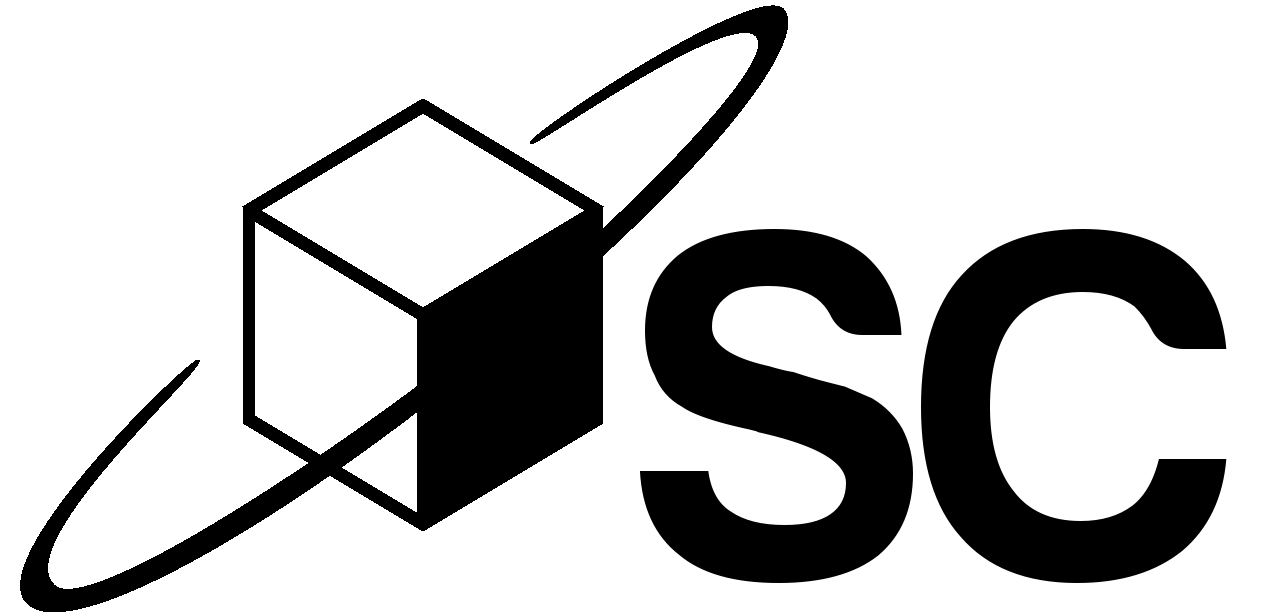
\includegraphics[height=2.66em]{template/sc.png}
    }
%    \vspace*{\fill}
}
\chead{
    \topskip0pt
    \vspace*{\fill}
    {
    \centering
        \small{
            THIS DOCUMENT IS INTENDED FOR INTERNAL USE ONLY
        }
    }
    \\
    {
    \centering
        \small{
        UNAUTHORIZED DISTRIBUTION OF THIS DOCUMENT IS STRICTLY PROHIBITED 
        }
    }
    \vspace*{\fill}
}
\rhead{
%    \topskip0pt
%    \vspace*{\fill}
    % right header content
    {
    \centering
        
\includegraphics[height=3.25em]{template/scrd.png}
    }
%    \vspace*{\fill}
}
\lfoot{
    % left footer content
    \topskip0pt
    \vspace*{\fill}
    SCRD
    Revision 0.1
    \vspace*{\fill}
}
\cfoot{
    % middle footer content
    \topskip0pt
    \vspace*{\fill}
    {
    \centering
    SCRD Internal Documents Template \\
    \today
    }
    \vspace*{\fill}
}
\rfoot{
    % right footer content
    \topskip0pt
    \vspace*{\fill}
    \thepage
    \vspace*{\fill}
}
% extend the header into the margins
\usepackage{calc}
\fancyheadoffset[L,R]{\marginparsep+\marginparwidth}

%--------------------------------------------------------------------------------------------------------------
%	My Packages
%--------------------------------------------------------------------------------------------------------------
\usepackage{capt-of}

%--------------------------------------------------------------------------------------------------------------
%
%	BEGIN DOCUMENT
%
%--------------------------------------------------------------------------------------------------------------
\begin{document}


%--------------------------------------------------------------------------------------------------------------
%
%	TITLE PAGE
%
%--------------------------------------------------------------------------------------------------------------
\begin{titlepage}

\newcommand{\HRule}{\rule{\linewidth}{0.5mm}} % Defines a new command for the horizontal lines, change thickness here

\center % Center everything on the page
 
%----------------------------------------------------------------------------------------
%	HEADING SECTIONS
%----------------------------------------------------------------------------------------

\includegraphics[width=200pt,height=200pt]{../images/rocketry_logo_large.png}\\[1cm] % Include a department/university logo - this will require the graphicx package
\textsc{\Large Space Concordia - Rocketry Division}\\[0.5cm] % Major heading such as course name
\textsc{\large Aurelius CR-2-4G - Structural Team}\\[0.5cm] % Minor heading such as course title

%----------------------------------------------------------------------------------------
%	LOGO SECTION
%----------------------------------------------------------------------------------------

\begin{figure}[ht]
    \centering
    \includegraphics[height=100pt]{../images/vertical_model_simplified.png}\\
\end{figure}

%----------------------------------------------------------------------------------------
%	TITLE SECTION
%----------------------------------------------------------------------------------------

\HRule \\[0.6cm]
{ \Huge \bfseries 
Engineering Simulation for Rocket Flight Analysis
}\\[0.4cm] 

\HRule \\[1cm]
 
%----------------------------------------------------------------------------------------
%	AUTHOR SECTION
%----------------------------------------------------------------------------------------

\begin{minipage}{0.4\textwidth}
\begin{flushleft} \large
	\begin{tabular} {r l} 
        \emph{Author(s):} & Shawn Bulger	\\
	\end{tabular}
\end{flushleft}
\end{minipage}
~
\begin{minipage}{0.4\textwidth}
\begin{flushright} \large
	\begin{tabular} {r l} 
		\emph{Coordinator:} & Dr. Ashok Kaushal 		\\
		\emph{Supervisor:}  & Dr. Mehdi Hojjati 		\\
		\emph{EIR:}         & Dominic Ng  		        \\
	\end{tabular}
\end{flushright}
\end{minipage}\\[2cm]

%----------------------------------------------------------------------------------------
%	DATE SECTION
%----------------------------------------------------------------------------------------

{\large \today}\\[2cm] % Date, change the \today to a set date if you want to be precise

\vfill % Fill the rest of the page with whitespace

\end{titlepage}

{
\hypersetup{linkcolor=black}
\setcounter{tocdepth}{2}
\tableofcontents
\clearpage
}
\listoftables
\listoffigures
\clearpage
\section{List of Abbreviations}\label{list-of-abbreviations}

\begin{longtable}[c]{@{}llll@{}}
\toprule
Abbreviation & Description & Function of & Units\tabularnewline
\midrule
\endhead
AOA, \(\alpha\) & Angle of Attack & & radians\tabularnewline
COP & Center of pressure & & N/A\tabularnewline
COG & Center of gravity & time & N/A\tabularnewline
Re & Reynolds Number & \( \rho,\mu,\vec{v},L \) &
dimensionless\tabularnewline
\(Re_{crit}\) & Critical Reynolds Number & \( \rho,\mu,\vec{v},L \) &
dimensionless\tabularnewline
\(I_{zz}\) & Pitch/Yaw Moment of Inertia & time & \(m^4\)\tabularnewline
D & Drag Force (combined) & & N\tabularnewline
W & Weight of the Rocket & & N\tabularnewline
R & Specific Gas Constant & & \(J kg^{-1} K^{-1}\)\tabularnewline
T & Thrust of the Rocket & & N\tabularnewline
\(t_f\) & Fin thickness & distance & m\tabularnewline
\(L_{cf}\) & Aerodynamic Chord Length of Fins & distance &
m\tabularnewline
c & Speed of sound & \( \sqrt{\gamma RT} \) &\tabularnewline
\(R_a\) & Surface Finish & \( distance \) & microns\tabularnewline
M & Mach Number & \( \vec{v}, c \) & dimensionless\tabularnewline
\(D_{pa}, C_{pa}\) & Parasitic Drag Force, Coefficient &
&\tabularnewline
\(D_{fb}, C_{fb}\) & Body Drag Force, Coefficient & &\tabularnewline
\(D_{fp}, C_{fp}\) & Fin Pressure Drag Force, Coefficient &
&\tabularnewline
\(D_{pr}, C_{pr}\) & Pressure Drag Force, Coefficient & &\tabularnewline
\(D_{in}, C_{in}\) & Interference Drag Force, Coefficient &
&\tabularnewline
\(D_{ba}, C_{ba}\) & Base Drag Force, Coefficient & &\tabularnewline
\(D_{sk}, C_{sk}\) & Skin Friction Drag Force, Coefficient &
&\tabularnewline
\(D_{aoa}, C_{aoa}\) & Additional Angle of Attack Drag Force,
Coefficient & &\tabularnewline
\(C_{MC}\) & Corrective Moment Coefficient & &\tabularnewline
\(C_{FN}\) & Normal Force Coefficient & &\tabularnewline
\(C_{PDM}\) & Propulsive Damping Moment Coefficient & &\tabularnewline
\(C_{ADM}\) & Aerodynamic Damping Moment Coefficient & &\tabularnewline
\(A_{wb}\) & Area of Wetted Body & & \(m^2\)\tabularnewline
\(A_{wf}\) & Area of Wetted Fins & & \(m^2\)\tabularnewline
\(A_{fr}\) & Frontal Reference Area & & \(m^2\)\tabularnewline
\(A_{fp}\) & Fin Planform Area & & \(m^2\)\tabularnewline
\(A_{fe}\) & Exposed Fin Planform Area & & \(m^2\)\tabularnewline
OD,\(\phi_{bt}\) & Outer Diameter & & m\tabularnewline
L & Total Length of Rocket & & m\tabularnewline
h\_n & Height of the nose cone & & m\tabularnewline
\(S_{fc}\) & Thrust Specific Fuel Consumption & &
\(\dfrac{g}{s}\cdot \dfrac{1}{N} = \dfrac{s}{m}\)\tabularnewline
\(\dot{m}_{fc}\) & Mass Flow Rate due to Fuel Consumption & &
\(\dfrac{g}{s}\cdot \dfrac{1}{N} = \dfrac{s}{m}\)\tabularnewline
\(T_{avg}\) & Average Thrust & & N\tabularnewline
\(t_{burn}\) & Burn Time & & s\tabularnewline
\(m_{m_t}\) & Total Motor Mass & & g\tabularnewline
\(W_{m_t}\) & Total Motor Weight & & N\tabularnewline
\(F_N\) & Aerodynamic Normal Force & & N\tabularnewline
\(F_A\) & Aerodynamic Axial Force & & N\tabularnewline
\(F_L\) & Aerodynamic Lift Force & & N\tabularnewline
\(S_{lm}\) & Longitudinal Stability Margin & & Calibers\tabularnewline
\(f_B\) & Fineness Ratio & & dimensionless\tabularnewline
\(\mu\) & Dynamic Viscosity & & \(N s / m^2\)\tabularnewline
\(\nu\) & Kinematic Viscosity & \(\mu\), \(\rho\) &
\(m^2/s\)\tabularnewline
\(\lambda\) & Angular Acceleration & & \(rad/s^2\)\tabularnewline
\(\omega\) & Angular Velocity & & \(rad/s\)\tabularnewline
\(\theta\) & Angular Position & & \(radians\)\tabularnewline
\bottomrule
\end{longtable}

\captionof{table}{List of Abbreviations}

\clearpage

\mainmatter

\chapter{Engineering Simulation for Rocket Flight
Analysis}\label{engineering-simulation-for-rocket-flight-analysis}

\section{Overview}\label{overview}

The goal of this project is to create an Engineering Simulation for
Rocket Flight Analysis in Matlab. This is not exactly a flight
simulator, which generally aims to train pilots and visually simulate
aircraft flight. An engineering simulation tests the dynamics and
behavior of a system, often employing a combination of analytic and
empirical methods, in order to validate an engineering model before its
deployment.

Such a simulation is driven by the requirements of the engineering
project. This project is constrained by the flight requirements of an
international rocketry competition, and as such, it is developed to
validate them.

A modular development pattern is performed where possible, in order to
support expansion for other simulation purposes. Unit and integration
testing of simulator logic is undertaken where reasonable, and further
validation is provided by testing the overall model against available
3rd party flight data.

Beyond the primary goal of validating the rocket flight performance
through simulation, this project is an educational tool to enhance the
knowledge and learning of the team members and of the \emph{Space
Concordia} society as a whole. Furthermore, it will serve as a starting
point for future controls and simulations applications to come, many of
which are discussed in the \textbf{Future Enhancements} section.

\section{Definition of the Problem}\label{definition-of-the-problem}

An engineering simulation is needed to predict the flight performance of
a high-powered rocket. A high-powered rocket is defined as having
between 160 Ns and 40,960 Ns total impulse {[}1{]}. A team from the
\emph{Space Concordia} association at \emph{Concordia University} is
entering a submission into the \emph{International Rocket Engineering
Competition} (IREC) run by the \emph{Experimental Sounding Rocket
Association} (ESRA). The competition provides performance targets which
must be met in order to be eligible to win. These targets are held as
design requirements for performance, and are listed in the
\textbf{Requirements} section below.

\section{Requirements}\label{requirements}

The Performance Model must provide the maximum altitude and velocity of
the rocket in subsonic flight under a known thrust curve and known
dimensional parameters.

\begin{itemize}
\tightlist
\item
  2a Static stability above 2 calibers
\item
  2b Dynamic stability above 0
\item
  2c Min velocity at launch rail 30.5 m/s
\item
  2d Vehicle max speed mach 0.9
\item
  2e Vehicle reaches 10,000 ft altitude (+1000 feet / - 0 feet)
\item
  2f Vehicle doesn't experience resonant pitching/yawing moment
\end{itemize}

{[}SCRD 2016 Specifications and Requirements{]}

\section{Validation}\label{validation}

\begin{itemize}
\tightlist
\item
  Sub-Models will be unit tested with 3rd party data to ensure
  functional validity where possible.
\item
  Once all Sub-Models are validated individually, the overall model will
  be validated using 3rd-party data.

  \begin{itemize}
  \tightlist
  \item
    Primary 3rd-party simulation data source will be OpenRocket
    simulations
  \item
    Where possible, actual 3rd-party rocket flight data will be used to
    validate the model
  \end{itemize}
\end{itemize}

\section{Problem Solving Approach}\label{problem-solving-approach}

\subsection{Kinematics}\label{kinematics}

\emph{Kinematics} is the study of the motion without consideration of
the forces in play. This analysis can be simplified by considering the
entire mass of a body at a convenient point, for instance the
\emph{Center of Gravity}. We call this the point-mass system. Of
particular interest are the position, velocity, and acceleration of the
point {[}2{]}.

\subsection{Dynamics}\label{dynamics}

\emph{Dynamics} is the study of motion which considers the forces in
play. It is useful to consider bodies as \emph{rigid bodies} in order to
simplify the forces that act on them (e.g.~ruling out the stiffness of
the body) {[}2{]}. Forces acting at a distance \(d\) from the center of
gravity create a rotation about the center of gravity.

\subsection{Decoupling the Model}\label{decoupling-the-model}

If it can be said that the translation of the body at its center of
gravity (kinematics) does not impact the rotation of the body about its
center of gravity by a force applied at some other point (the
\emph{Center of Pressure}), the analysis can be greatly simplified. Such
a \emph{mutually independent system of equations} could be solved rather
easily, as the translational model could be solved independently of the
rotational model, and vice-versa {[}2{]}. Coupled systems of equations,
on the other hand, would have to be solved simultaneously.

As it happens, the translational model of the rocket is not fully
decoupled from the rotational model. As the rocket rotates while
travelling through the air at an angle of attack, it presents a larger
reference area and thus increases the drag force, causing a negative
acceleration in the translational point-mass model. Likewise, an
increase in the translational velocity of the rocket creates a larger
lift force when the rocket is rotating at an angle of attack. This lift
force, which is applied at the rocket's center of pressure, creates a
rotation about the center of gravity.

However, it is possible to proceed with a decoupled analysis with the
assistance of careful assumptions and approximations within acceptable
accuracy. If accepted, this would imply a \emph{weak coupling} between
the translational model and the rotational model {[}2{]}.

\section{Assumptions}\label{assumptions}

\begin{itemize}
\tightlist
\item
  subsonic flight
\item
  axis-symmetric rigid body rocket
\item
  single cylindrical body
\item
  Von Karman nose shape
\item
  three or four trapezoidal fins
\item
  passively controlled (no active thrust or stability control)
\item
  constant fuel expenditure rate
\item
  vertical/linear flight within 5 degrees {[}3{]}
\item
  the \emph{Ideal Gas Law} applies throughout the flight
\item
  humidity in the air is ignored
\item
  steady-state irrotational flow around the body {[}4{]}
\item
  fully aligned thrust {[}3{]}
\item
  smooth transition between nose cone and body tube (no shoulder)
\item
  rocket does not have a boattail
\item
  rocket has a single rectangular launch lug
\end{itemize}

\chapter{Input Parameters}\label{input-parameters}

Before beginning the modeling process, it is necessary to understand the
inputs of the system.

Many parameters can be considered unchanging during flight, and are from
this point referred to as \emph{Static Parameters}. Other inputs change
as a function of time or velocity, and must be carefully handled within
the system - these parameters are herein referred to as \emph{Dynamic
Parameters}.

\section{Atmospheric Model}\label{atmospheric-model}

The \emph{International Standard Atmosphere} model is assumed to
describe the pressure, temperature, density and viscosity conditions of
the surrounding air during launch.

{[}5{]}

\subsection{Viscosity}\label{viscosity}

Previously, in-house simulations were conducted using the
\emph{velocity\_model} created by Alex Botros. Of interest to this
report, is the method by which the viscosity of the working fluid was
calculated. It will include a review of the previous methods use and it
will introduce \emph{Sutherland's law}. As well, both methods will be
compared and changes to the existing model will be proposed.

\subsection{Previous Work}\label{previous-work}

In the \emph{velocity\_model} the absolute viscosity was never actually
calculated. Instead, the kinematic viscosity was calculated (as shown
below) as part of the function to solve for the \emph{Reynolds Number}
of the vehicle.

\begin{equation}
\label{kinematic_viscosity_f_T}
\nu = (-1 E -14) T^3 + (1 E -10) T^2 + (3 E -8) T - (3 E -6)
\end{equation}

As can be clearly seen, the kinematic viscosity was estimated based on
the temperature T. It is assumed that the temperature is in Kelvin. When
the function shown here is plotted, it creates the following result.

\section{Static Parameters}\label{static-parameters}

Many rocket design parameters are considered to remain constant during
flight.

These parameters are written in the parametric spreadsheet shared with
the design team. The CAD software populates values related to the
structural design, and others are entered manually. The performance
model reads them at the beginning of execution to simulate the latest
design iteration.

Find the included file named `Parametric\_Model.xlsx'

\section{Dynamic Parameters}\label{dynamic-parameters}

Parameters listed as \emph{dynamic} in the table above are provided as
initial values which are then recalculated by the model throughout the
simulated flight.

\subsection{Force}\label{force}

\emph{Force} is a change in momentum with time, and is related by
Newton's Second Law

\begin{equation}
F = \dfrac{m \Delta \vec{v}}{\Delta t} = m\vec{a}
\end{equation}

\subsection{Impulse}\label{impulse}

\emph{Impulse} is the product of force and integration of a differential
(infinitesimal period) of time between the time periods in which it was
applied.

\begin{equation}
\label{impulse}
J = \int^{t_2}_{t_1} F dt
\end{equation}

This is also known as the \emph{Total Impulse}, or the \emph{total
change in momentum}, and can be calculated as the average thrust over a
given time period.

\subsection{Thrust}\label{thrust}

Thrust is the mechanical force that drives the flight of the rocket. It
is a vector quantity of magnitude and direction. \emph{Thrust} is a
reaction force in the opposite direction of accelerating fluid (exhaust
gas) caused by the combustion of fuel, and is assumed to be aligned with
the longitudinal axis of the rocket.

\subsection{Mass Flow Rate}\label{mass-flow-rate}

\emph{Mass Flow Rate} is found by the product of fluid density,
velocity, and cross-sectional area.

\begin{equation} 
\dot{m} = \rho \vec{v} A
\end{equation}

{[}6{]}

\subsubsection{Thrust Equation}\label{thrust-equation}

Thrust is a mechanical force created by a propulsion system which moves
a vessel through a medium. In high-powered rocketry, it is typically
created by the expulsion of hot gas generated during the ignition of a
solid fuel motor. The acceleration of gases from the motor causes a
thrust force in the opposite direction (according to Newton's 2\(^{nd}\)
law), which propels the rocket from the launch pad. The thrust force is
the product of the mass flow rate of the hot gases and the change in
velocity between the exit of the nozzle and the free stream.

\begin{equation} 
T = \dot{m} \Delta \vec{v} 
\end{equation}

{[}6{]}

Thrust curves are provided by the manufacturer, based on static tests.
The highest performing result from the batch of test motors is chosen
for the curve. Therefore, the thrust curve represents the highest
expected performance of the motor within the specified operating
conditions

Table \ref{sample_motor_data} shows an example of the motor data
provided by ThrustCurve.org:

\begin{longtable}[c]{@{}ll@{}}
\toprule
Parameter & Value\tabularnewline
\midrule
\endhead
Manufacturer & Cesaroni Technology\tabularnewline
Entered & May 20, 2009\tabularnewline
Last Updated & Jun 26, 2014\tabularnewline
Mfr. Designation & 6819M1540-P\tabularnewline
Common Name & M1540\tabularnewline
Motor Type & reload\tabularnewline
Delays & P\tabularnewline
Diameter & 75.0mm\tabularnewline
Length & 75.7cm\tabularnewline
Total Weight & 5906g\tabularnewline
Prop. Weight & 3624g\tabularnewline
Cert. Org. & Canadian Association of Rocketry\tabularnewline
Cert. Designation & 6819-M1540-IM-P\tabularnewline
Cert. Date &\tabularnewline
Average Thrust & 1537.0N\tabularnewline
Maximum Thrust & 2328.8N\tabularnewline
Total impulse & 6819.4Ns\tabularnewline
Burn Time & 4.4s\tabularnewline
Case Info & Pro75-5G\tabularnewline
Propellant Info & Imax\tabularnewline
Availability & regular\tabularnewline
\bottomrule
\end{longtable}

\captionof{table}{\label{sample_motor_data}Sample Motor Data}

\begin{figure}[htbp]
\centering
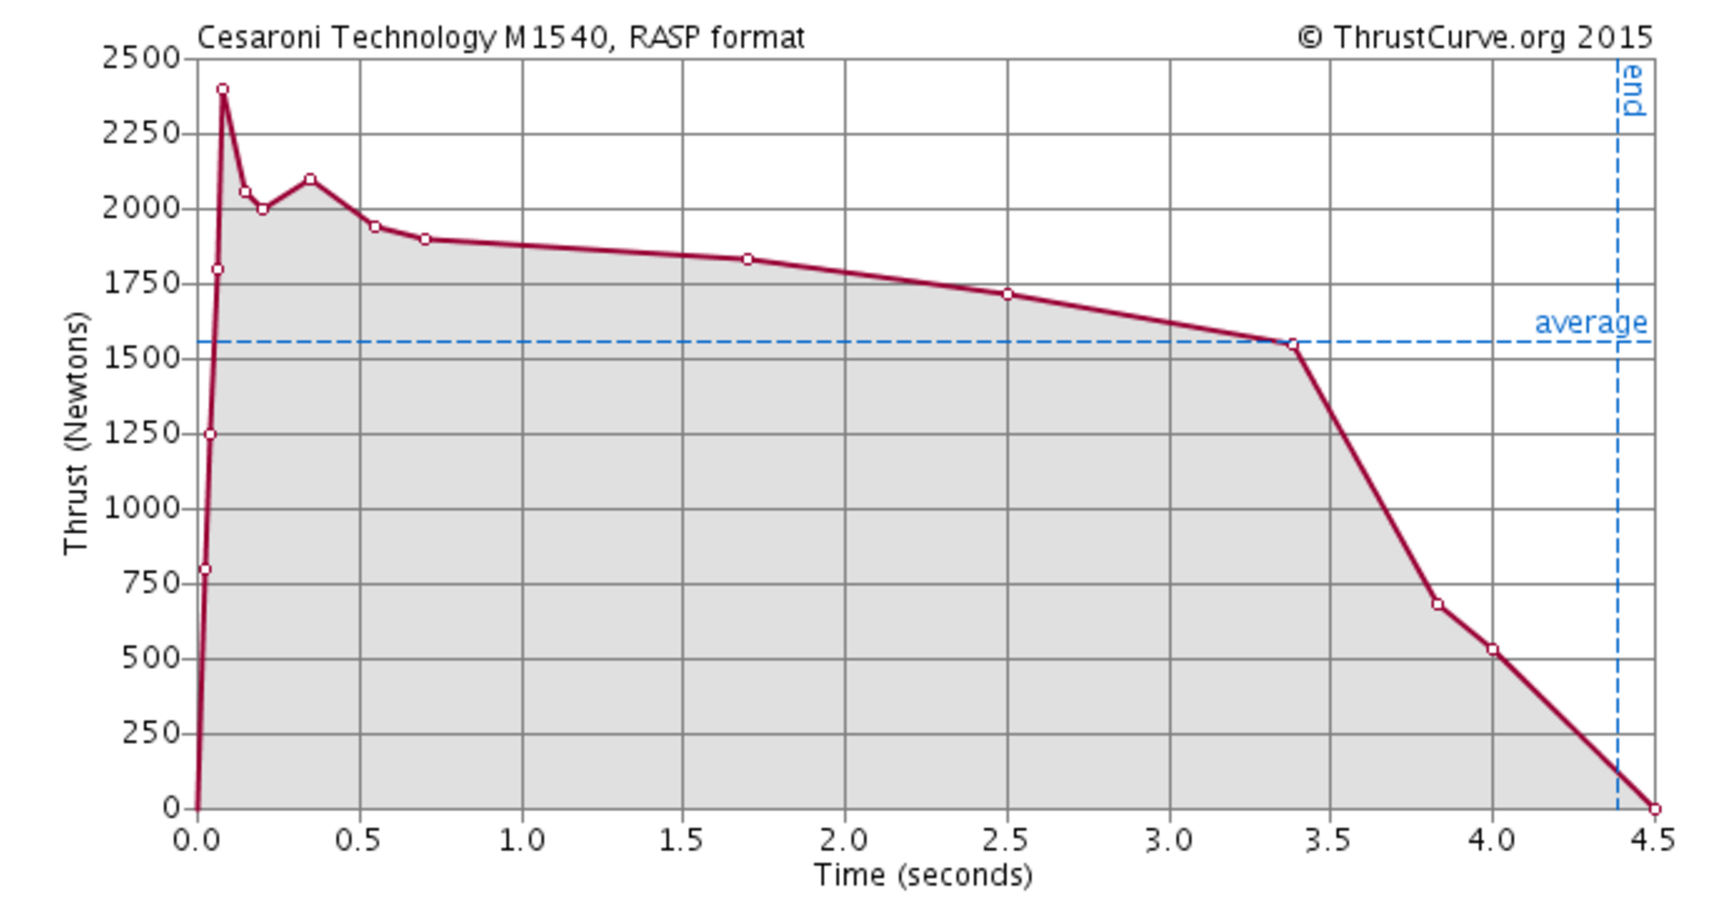
\includegraphics{images/M1540_thrust_curve.png}
\caption{Sample Thrust Curve\label{thrust_curve_label}}
\end{figure}

Source: http://www.thrustcurve.org/motorsearch.jsp?id=673

\paragraph{Thrust Specific Fuel
Consumption}\label{thrust-specific-fuel-consumption}

\emph{Thrust Specific Fuel Consumption} is how much fuel is burned for a
given time.

\begin{equation}
S_{fg} = \dfrac{m}{t_{burn}}\cdot \dfrac{1}{T_{avg}}  
\end{equation}

\begin{equation}
\left[ \dfrac{g}{s}\cdot \dfrac{1}{N} = \dfrac{s}{m} \right]  
\end{equation}

Since at the time of writing the \(S_{fc}\) was not provided by the
manufacturer, the following calculations are used for a first
approximation.

\subparagraph{Assumptions}\label{assumptions-1}

\begin{itemize}
\tightlist
\item
  all propellant is spent during the motor burn time
\item
  final \(S_{fg}\) determined is constant during burn
\item
  the motor info provided is accurate
\end{itemize}

\begin{quote}
It should be noted that a variance in thrust of \(\pm 20 \%\) is
possible. This and other variance factors are taken into account in the
\emph{Statistical Analysis} section.
\end{quote}

From the table above, the dry propellant weight is given as 3624 grams.
The Average Thrust is given as 1537.0 Newtons, and the total burn time
is given as 4.4 seconds.

Thus, the \emph{Thrust Specific Fuel Consumption} can be determined as
follows:

\begin{equation}
S_{fg} = \dfrac{3.624 \, kg}{4.4 \, s} \cdot \dfrac{1}{1537.0 \, N} \approx 0.00053587 \dfrac{kg}{N \cdot s} = 5.3587 \times 10^{-4} \dfrac{kg}{N \cdot s} 
\end{equation}

This rate is considered constant.

\subsection{Weight}\label{weight}

As fuel is expended in generating thrust, the weight of the rocket is
reduced. One assumption that can be made is that the change of mass with
time is ``proportional to the impulse of the motor up to that point''
{[}3{]}.

\begin{equation}
\label{eq_mass_burned}
\Delta M_i = - \dfrac{M_f \int^i_0 T dt}{\int^\infty_0 T dt}
\end{equation}

Where:

\begin{itemize}
\tightlist
\item
  \(M_f\) is the total mass of fuel
\item
  \(T\) is the thrust
\item
  \(\Delta M_i\) is the change in mass of fuel between time \(i\) and
  \(t\)
\end{itemize}

{[}3{]}

We can also use the \emph{Thrust Specific Fuel Consumption} to determine
the corresponding reduction in weight during burn, if we assume that the
mass flow rate of fuel during burn is constant.

First remove the Average Thrust term to isolate the mass flow rate:

\begin{equation}
\dot{m} = S_{fG} \cdot T_{avg} = 5.3587 \times 10^{-4} \dfrac{kg}{N \cdot s} \cdot 1537.0 \, N  = 0.8236 \, kg/s 
\end{equation}

This equation can be expressed in terms of Weight through Newton's
2\(^{nd}\) law: \(F = m\vec{a}\)

\begin{equation}
\dot{W}_m = \dot{m} \cdot \vec{g} = 0.8236 \, kg/s \cdot 9.81 \, m/s^2 \approx 8.0799 N/s 
\end{equation}

To develop a relation for the change in weight as a function of
\(S_{f_c}\)

\begin{equation} 
W_f(t) = (m_{f_i} kg - \Delta m(t)) \cdot \vec{g} 
\end{equation}

\begin{equation}
W_f(t) = (3.624 \, kg - \Delta m(t)) \cdot 9.81 \, m/s^2 
\end{equation}

\begin{equation}
W_f(t) = W_{f_i} - \Delta W_f(t)
\end{equation}

\begin{equation}
\Delta W_f (t) = \int \dot{W} dt = \dot{W}\cdot t
\end{equation}

\begin{equation}
\Delta W_f (t) = \dfrac{\Delta m(t) \cdot \vec{g}}{t}\cdot t = \Delta m (t) \cdot g 
\end{equation}

\begin{equation}
\Delta m_f(t) = S_{fg} \cdot t
\end{equation}

Finally, the motor weight as a function of time is

\begin{equation}
W_m (t) = W_{m_t} - \Delta W_f(t) = W_{m_t} - \dot{m}_{fc} \cdot t
\end{equation}

As a further simplification, if we assume that the mass flow rate is
constant, we can find it simply by dividing the mass propellant by the
motor burn time. This results in only a slight error as shown in Figure
\ref{dynamic_weight_calculation_test_figure_label} below.

Figure \ref{dynamic_weight_calculation_test_figure_label} shows the
output of the dynamic weight calculation in Matlab. The Thrust and
Weight curves produce output similar to OpenRocket as expected.

\begin{figure}[htbp]
\centering
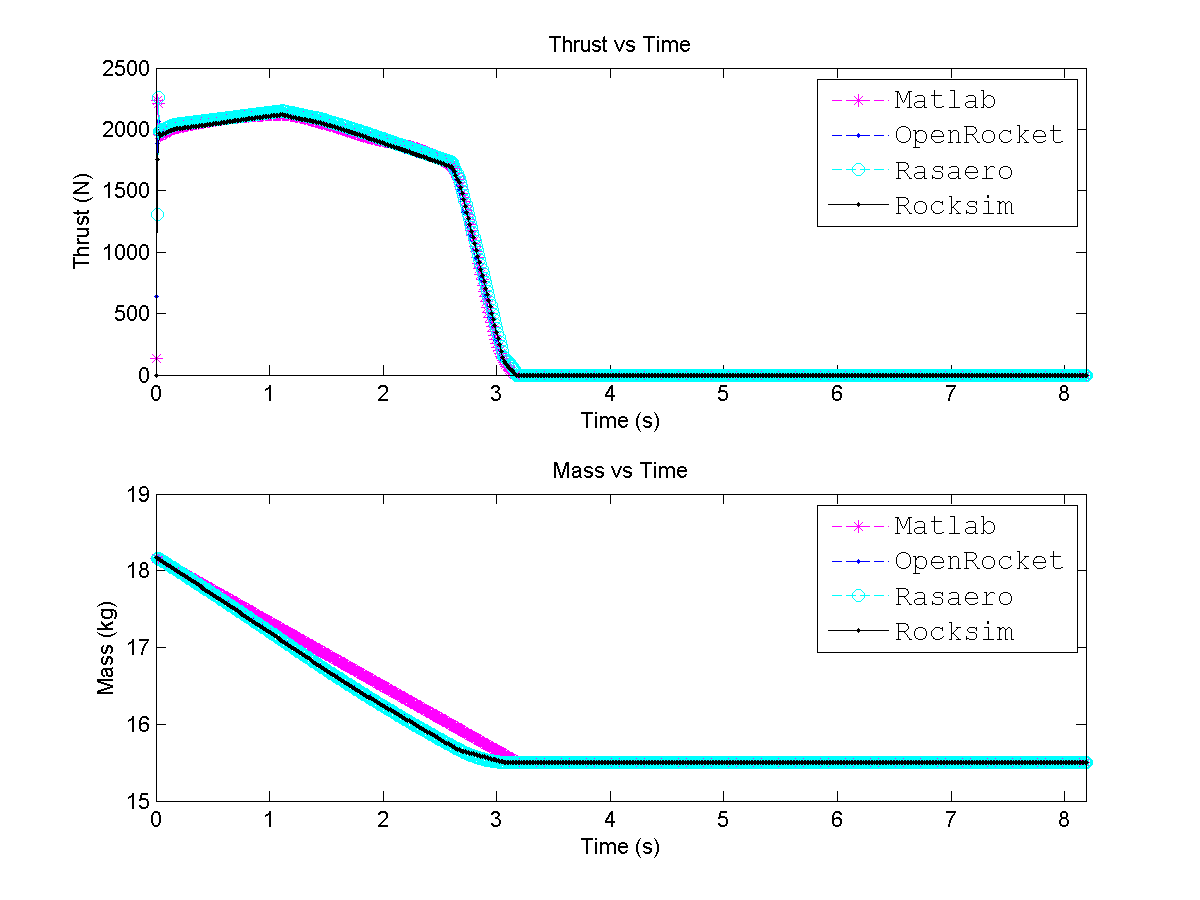
\includegraphics{images/plots/error_thrust_mass.png}
\caption{Dynamic Weight Calculation Test Output
\label{dynamic_weight_calculation_test_figure_label}}
\end{figure}

\subsection{Center of Gravity}\label{center-of-gravity}

The \emph{Center of Gravity} is a location were we can consider the
entire rocket mass to be concentrated in a point-mass system.

\begin{equation}
y_{cg} = \dfrac{m_1 y_1 + m_2 y_2 + ... + m_n y_n}{\sum_{j=1}^n m_j}
\end{equation}

\begin{equation}
COG(t) = \dfrac{m_1 y_1 + (m_2 - \Delta m) y_2}{m_1 + m_2 - \Delta m(t)} 
\end{equation}

Where COG(t) is the Center of Gravity as a function of time, \(m_1\) is
the static mass (combination of nose cone, body tube, and fins), \(m_2\)
is the initial mass of the motor, and \(\Delta m(t)\) is the change of
mass as a function of time due to fuel expenditure.

We consider the motor as a point mass centered at the geometric center
of the motor casing. This simplifies the calculation of the center of
gravity of the rocket as fuel is expended, as only the mass of the motor
is changing, and not the location of its particular center of mass.

\subsection{Moments of Inertia}\label{moments-of-inertia}

The instantaneous moment of inertia is determined by relating the moment
of inertias of the static structure and the dynamic structure through
the parallel axis theorem evaluated at the total center of gravity
(COG).

The sum of moment of inertias evaluated through the \emph{parallel axis
theorem} nets the total rocket moment of inertia.

\begin{equation}
\label{eq_parallel_axis_theorem}
I_n = I_{cm(n)} + M_P d^2 
\end{equation}

\begin{equation}
I_T(t) = \sum I_n 
\end{equation}

Where:

\begin{itemize}
\tightlist
\item
  \(I_T(t)\) is the total moment of inertia of the rocket as a function
  of time
\item
  \(I_n\) is the component vector (either static or dynamic moment of
  inertia)
\end{itemize}

{[}3{]}

\subsubsection{Longitudinal Moment of
Inertia}\label{longitudinal-moment-of-inertia}

To the \emph{Moment of Inertia} related to the pitch/yaw of the rocket
is the \emph{Longitudinal Moment of Inertia}.

\begin{equation}
\label{longitudinal_moment_inertia}
I = \dfrac{mL^2}{12}
\end{equation}

{[}TODO source dynamics textbook{]}

In keeping with the assumption of the motor as a point mass in the
volumetric center of the motor casing, the dynamic \emph{Longitudinal
Moment of Inertia} is calculated as follows.

\begin{equation}
\label{static_longitudinal_moment_inertia}
I_{s} + m_{s} r_{0 \rightarrow 1}^2
\end{equation}

Where \(r_{0 \rightarrow 1}\) is the distance between the static center
of gravity (the COG of the nose cone, body tube, and fins) and the
instantaneous center of gravity of the rocket. \(I_{s}\) is provided by
CATIA.

\begin{equation}
\label{motor_longitudinal_moment_inertia}
I_{m} = \dfrac{m_{m}L_{m}}{12} + m_{m}r_{0 \rightarrow 2}^2
\end{equation}

Where \(L_{motor}\) is the length of the motor casing, and
\(r_{0 \rightarrow 2}\) is the distance between the motor center of
gravity and the rocket center of gravity.

Then, the rocket \emph{Longitudinal Moment of Inertia} is the sum, shown
as follows

\begin{equation}
\label{rocket_longitudinal_moment_inertia}
I_{r} = I_{m} + I_{s}
\end{equation}

\subsection{Center of Pressure}\label{center-of-pressure}

The \emph{Center of Pressure} (COP) is the location (point) where the
aerodynamic forces can be said to be acting, simplifying the complex
distribution of forces across the rocket and its features.

The \emph{Center of Pressure} changes with the normal force distribution
on the rocket, which is driven by \emph{Angle of Attack} {[}7{]}.

\[ COP = COP(\alpha) \]

A wind tunnel is the best way to approximate this point, but an analytic
method is available, discussed in detail in the next section.

Figure \ref{cop_cog_il_figure} shows how our determination of the
\(COP\), \(COG\), and \(I_L\) compares with other simulation software.

\begin{figure}[htbp]
\centering
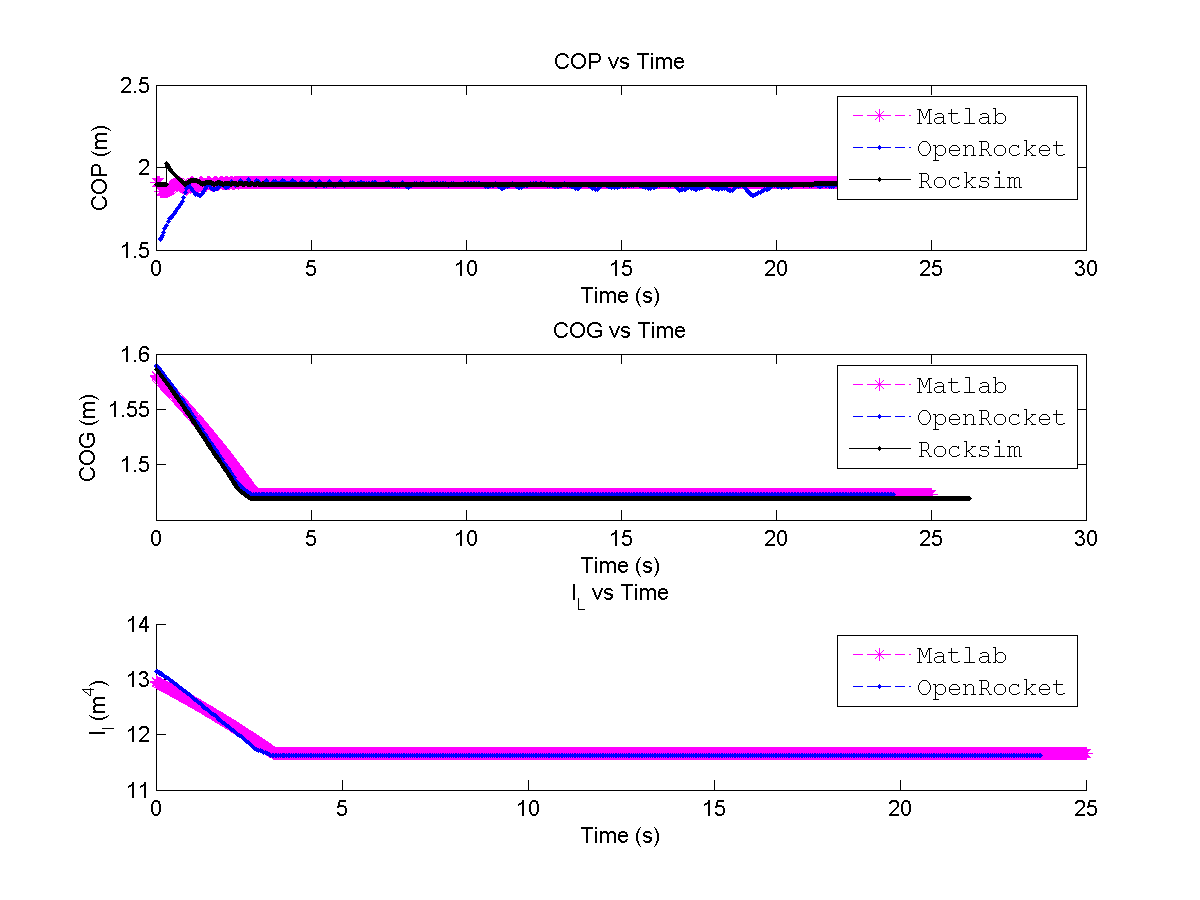
\includegraphics{images/plots/error_cog_cop_il_plot.png}
\caption{COP, COG, and I\_l as a function of time
\label{cop_cog_il_figure}}
\end{figure}

\clearpage

\chapter{The Barrowman Method}\label{the-barrowman-method}

In 1966, James Barrowman published a report called ``The Theoretical
Prediction of the Center of Pressure'' {[}8{]}. Despite some
modifications and additions since, it remains a fundamental method, ever
present in modern high-powered rocketry.

\emph{Barrowman's Method} is principally used to determine the
\emph{Center of Pressure}.

\begin{equation}
\label{rocket_center_of_pressure}
\bar{X} = 
\dfrac
{ \left( C_{N \alpha} \right)_n \bar{x}_n + \left( C_{N \alpha} \right)_{cb} \bar{x}_{cb} + \left( C_{N \alpha} \right)_{fb} \bar{x}_{fb} }
{ C_{N \alpha}  }
\end{equation}

Where:

\begin{itemize}
\tightlist
\item
  \(C_{N \alpha}\) is the \emph{Stability Derivative}
\item
  subscript \(_n\) refers to the nose cone
\item
  subscript \(_{cb}\) refers to the cylindrical body
\item
  subscript \(_{fb}\) refers to the fin set in the presence of the body
\item
  \(\bar{x}\) refers to the component centroid
\end{itemize}

{[}7{]}

\section{Stability Derivative}\label{stability-derivative}

The \emph{Stability Derivative} \(C_{N\alpha}\) is a dimensionless
parameter, used to calculate the force normal to the longitudinal axis,
and is dependent on the shape of the component. It is the slope of the
\emph{Normal Force Coefficient} plotted against the angle-of-attack. For
low angles of attack, it is nearly constant.

TODO show figure

{[}2{]}

The total \emph{Stability Derivative} is the sum of all \emph{i} rocket
component stability derivatives

\begin{equation}
\label{total_stability_derivative}
C_{N \alpha} = \sum C_{N \alpha (i)}   
\end{equation}

{[}3{]}

\section{Nose Cone}\label{nose-cone}

\begin{equation}
\label{eq_sd_nosecone}
C_{N \alpha (n)} = 2
\end{equation}

\section{Rocket Body}\label{rocket-body}

The \emph{Barrowman Method} considers the body lift at small angles of
attack to be negligible.

\begin{equation}
\label{eq_sd_bodytube}
C_{N \alpha (bt)} = 0
\end{equation}

\section{Fins}\label{fins}

The following solution for the fin set stability derivative applies only
for identically shaped fins, in sets of 3, 4, or 6.

\begin{equation}
\label{eq_sd_fin_set}
C_{N \alpha(f)} = C_{in}\dfrac{4n \left( \dfrac{s}{d} \right)^2}{1 + \sqrt{1 + \left( \dfrac{2 l}{a + b} \right)^2}}
\end{equation}

Where:

\begin{itemize}
\tightlist
\item
  \(a\) is the fin tip chord length
\item
  \(b\) is the fin root chord length
\item
  \(s\) is the fin height
\item
  \(l\) is the distance between the root center and the tip center
\item
  \(C_{in}\) is a coefficient for the interference effects of the air
  flow near the fin-body interface
\end{itemize}

{[}7{]}

\begin{equation}
\label{eq_sd_interference}
C_{in} = 1 + \dfrac{OD/2}{OD/2 + s}
\end{equation}

{[}7{]}

\section{Nose Cone COP}\label{nose-cone-cop}

\subsection{LV-Haack Nose Cone COP}\label{lv-haack-nose-cone-cop}

\begin{equation}
\label{eq_cop_lv_haack}
\bar{X}_n = 0.437 h_n
\end{equation}

{[}9{]}

\subsection{Von Karman Nose Cone COP}\label{von-karman-nose-cone-cop}

\begin{equation}
\label{eq_cop_von_karman}
\bar{X}_n = 0.500 h_n
\end{equation}

{[}9{]}

\subsubsection{Fin Set COP}\label{fin-set-cop}

The location of the \emph{Center of Pressure} for the fin set is as
follows.

\begin{equation}
\label{eq_cop_fin_set}
\bar{X}_{fb}
= 
X_f 
+ 
\dfrac {m ( b + 2 a )} {3 ( b + a ) } 
+ \dfrac{1}{6} 
\left[ b + a - \dfrac{b a}{b + a} \right]
\end{equation}

{[}3{]}

Where:

\begin{itemize}
\tightlist
\item
  \(X_f\) is the distance from the tip of the nose cone to the point
  where the leading edge of the fin meets the body tube {[}3{]}
\item
  \(a\) is the fin tip chord length
\item
  \(b\) is the fin root chord length
\item
  \(s\) is the fin height
\item
  \(m\) is the fin sweep length
\end{itemize}

Also, see this
\href{http://physics.gallaudet.edu/tools/rocketcop.html}{Center of
Pressure Calculator online}.

\paragraph{Cylindrical Body COP}\label{cylindrical-body-cop}

The centroid of a cylindrical body will be half its length

\begin{equation}
\label{eq_centroid_bodytube}
\bar{x}_{ct} = \dfrac{1}{2} l_{cb}
\end{equation}

Wind tunnel tests performed in 1918 and 1919 demonstrated that the
normal force generated by a cylindrical body at an angle of attack of
less than 10 degrees is negligible

{[}7{]}.

\section{Rocket Body Lift Correction}\label{rocket-body-lift-correction}

\emph{Barrowman's Method} neglects the lift generated by the rocket
body. Galejs {[}10{]} suggests the following adjustment to provide a
compensated \emph{Coefficient of Normal Force due to Body Lift}

\begin{equation}
\label{eq_coef_normal_force_body_lift}
C_{N(L)} = K \dfrac{A_p}{A_ref} \alpha^2
\end{equation}

Where:

\begin{itemize}
\tightlist
\item
  \(K\) = 1
\item
  \(A_p\) is the rocket planform area excluding the fins
\item
  \(A_{ref}\) is the reference area of the rocket
\end{itemize}

{[}3{]}

Equation \ref{eq_coef_normal_force_body_lift} is divided by \(\alpha\)
to be added to \(C_{N \alpha}\) calculated and used in Equation
\ref{rocket_center_of_pressure}.

TODO All COP components must be modified by the lift coefficient

\begin{equation}
\label{eq_coef_normal_force_body_lift_alpha}
C_{N \alpha^2} = K \dfrac{A_p}{A_ref} \alpha
\end{equation}

This correction is applied at the centroid of the planform area.

{[}3{]}

\section{Transonic Considerations}\label{transonic-considerations}

\emph{Barrowman's Equations} are based on assumptions that are only
valid in subsonic flight. In the transonic and supersonic regions, what
new effects are introduced that would affect the location of the
\emph{Center of Pressure}?

\section{Aerodynamic Geometry}\label{aerodynamic-geometry}

\subsection{Overview}\label{overview-1}

Related to aerodynamic geometry of the rocket, the specific parameters
of interest are the following:

\begin{itemize}
\tightlist
\item
  Outer Diameter of Rocket (\emph{OD})
\item
  Total Length of Rocket (\emph{L})
\item
  Height of Nose Cone (\(h_n\))
\item
  Thickness of Fins
\item
  Number of Fins
\item
  Width of Fins
\item
  Surface Area of Nose
\end{itemize}

\subsection{Surface Roughness}\label{surface-roughness}

\emph{Surface Roughness} is the deviation in the normal direction from a
surface of its features. It contributes to \emph{Skin Friction Drag}

\subsection{Fineness Ratio}\label{fineness-ratio}

The \emph{Fineness Ratio} is the ratio of the length to the outer
diameter

\begin{equation} 
f_B = \dfrac{L} {OD}
\end{equation}

\subsection{Fins}\label{fins-1}

\subsection{Aerodynamic Chord Length of
Fins}\label{aerodynamic-chord-length-of-fins}

Since there is no airfoil on the fin design, the \emph{Aerodynamic Chord
Length of the Fins} (\(L_{cf}\)) is equal to the height of the fins.

\subsection{Areas}\label{areas}

Reference areas are required to calculate the drag force.

\subsubsection{Wetted Body Area}\label{wetted-body-area}

The \emph{Wetted Body Area} is the combined area of all surfaces in
contact with moving air.

\subsubsection{Frontal Reference Area}\label{frontal-reference-area}

The \emph{Frontal Reference Area} is the projected area of the rocket
perpendicular to the direction of air flow. For perfectly vertical
flight and quiescent air conditions, this is the precise projection of
the tip face of the rocket.

{[}TODO show figure{]}

\paragraph{Frontal Reference Area at Angle of
Attack}\label{frontal-reference-area-at-angle-of-attack}

When the rocket pitches into the free stream at an angle of attack, a
greater portion of the rocket comprises the frontal reference area. We
do not account for this, as it would be extremely complex to evaluate.
We consider the frontal reference area does not change with
angle-of-attack.

\subsubsection{Planform Area}\label{planform-area}

\section{Nose Profile}\label{nose-profile}

\subsection{Von Karman (Haack)}\label{von-karman-haack}

A \emph{Von Karman} nose profile has been selected by the design team,
other profiles will not be supported in the initial version of the
model. The \emph{Von Karman} nose profile is a \emph{Haack Series}
geometry, designed to minimize theoretical pressure drag
{[}niskanen2013{]}. This profile excels in subsonic flow conditions, and
performs well in transonic flow conditions {[}nassaNoseCone{]} - as such
is it well suited for the current mission.

The equation for the \emph{Haack Series} is

\begin{equation}
r(x) = \dfrac{R}{\sqrt{\pi}} \sqrt{ \theta - \dfrac{1}{2} sin (2 \theta) + \kappa \sin^3 \theta }
\end{equation}

Where

\begin{equation}
\theta = \cos^{-1} \left( 1 - \dfrac{2x}{L} \right)
\end{equation}

\href{http://rimworld.com/nassarocketry/fabrication/nosecones/design.html}{Nose
Profile Design}

\href{https://en.wikipedia.org/wiki/Nose_cone_design\#Von_K.C3.A1rm.C3.A1n}{Nose
Profile Design}

\subsection{Aerodynamic Center}\label{aerodynamic-center}

The \emph{Aerodynamic Center} is the point where the \emph{Pitching
Moment} does not change with angle-of-attack

Sources:

\begin{itemize}
\tightlist
\item
  http://ocw.mit.edu/courses/aeronautics-and-astronautics/16-100-aerodynamics-fall-2005/lecture-notes/16100lectre10\_cg.pdf
\item
  http://www.digplanet.com/wiki/Aerodynamic\_center
\end{itemize}

\chapter{Drag Model}\label{drag-model}

Rockets in flight experience multiple sources of drag. The total drag
effect is the sum of all specific drag effects.

Figure \ref{rocket_drag_sources_label} depicts the types of drag forces
to be expected in subsonic flight at \emph{zero-angle of attack}.

\begin{figure}[htbp]
\centering
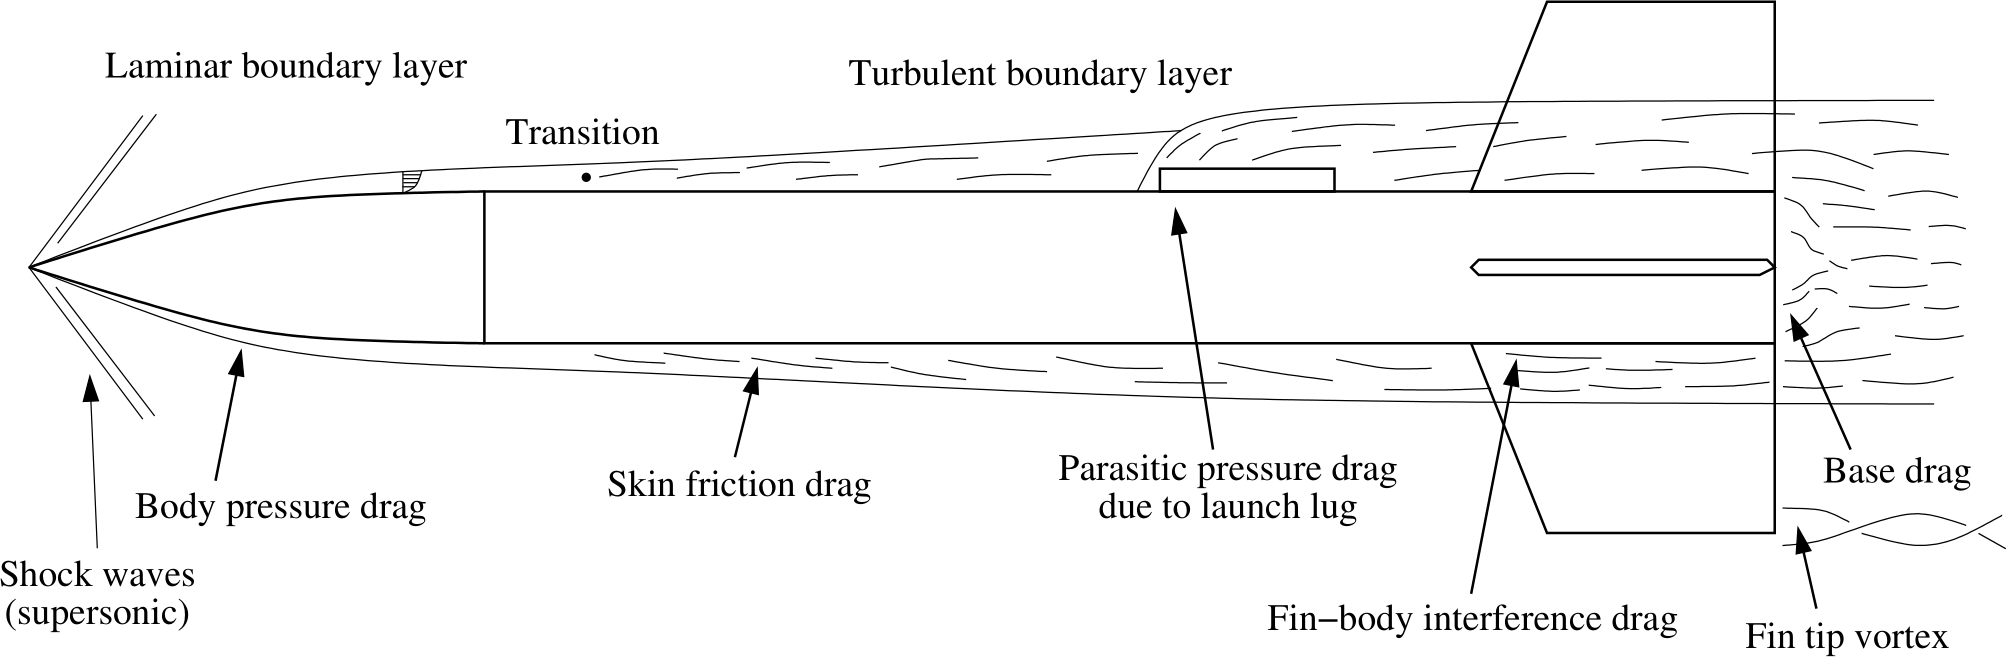
\includegraphics{images/drag_sources_niskanen2013.png}
\caption{Rocket Drag Sources - Subsonic Flight
\label{rocket_drag_sources_label}}
\end{figure}

{[}4{]}

The two main contributing factors to \emph{Drag Force} are \emph{Skin
Friction} and pressure distribution effects. Pressure distribution
effect are broken down into body pressure and parasitic drag effects,
among others {[}4{]}. These and other drag forces are detailed in this
section.

The drag model must take the parametric design parameters and applicable
dynamics parameters (see \emph{Data Model}) to output the Drag Force and
combined drag coefficient.

\section{Mach Number}\label{mach-number}

\emph{Mach Number} (M) is the ratio of the airspeed to the speed of
sound for air at a given temperature

The speed of sound (c) is calculated as follows

\begin{equation}
c = \sqrt{\gamma R T } 
\end{equation}

The \emph{Ideal Gas Law} states that

\begin{equation}
\label{ideal_gas_law}
P = \rho R T
\end{equation}

We assume that the \emph{Ideal Gas Law} applies, and use it to solve for
\emph{RT} using pressure and density. \[ RT = \dfrac{P}{\rho} \]

Thus we can calculate the speed of sound as follows

\begin{equation}
\label{speed_of_sound}
c = \sqrt{\gamma \dfrac{P}{\rho} } 
\end{equation}

Where \(p\) is the local pressure, \(\rho\) is the local density, and
\(\gamma\) is the \emph{adiabatic index}, known as the \emph{isentropic
explansion factor} - it is the ratio of the specific heats of a gas at
constant pressure and constant volume.

{[}11{]}

The \emph{Mach Number} is then the ratio of the air velocity to the
sound speed of the local air

\begin{equation}
M = \dfrac{ \vec{v} } { c }
\end{equation}

\subsection{Mach Regions}\label{mach-regions}

\emph{Velocity regions} are defined, in which aerodynamic effects are
known to vary considerably. The following velocity regions are
established for further discussion.

\begin{longtable}[c]{@{}ll@{}}
\toprule
Mach Region (\emph{M}) & Classification\tabularnewline
\midrule
\endhead
0.3 \textless{} 0.8 & Subsonic\tabularnewline
0.8 \textless{} M \textless{} 1 & Transonic\tabularnewline
1 \textless{} M \textless{} \textasciitilde{}5 &
Supersonic\tabularnewline
M \textgreater{} \textasciitilde{}5 & Hypersonic\tabularnewline
\bottomrule
\end{longtable}

\captionof{table}{Mach Regions}

{[}4{]}

As the rocket is constrained not to exceed Mach 0.9, much of the flight
will be in the subsonic region, greatly simplifying much of the
analysis. However, transonic effects cannot be ignored when at a Mach
Number greater than 0.8.

\clearpage

\section{Incompressible Flow}\label{incompressible-flow}

For Mach \textless{} 0.3,

\begin{quote}
In the incompressible flow regime the forces can be divided into
pressure force and viscous force
\end{quote}

\emph{Pressure Force} is due to fluid stagnation on areas of the rocket,
as well as due to the low pressure region created beyond the rocket at
is passes quickly through the air.

\emph{Viscous Force} is due to boundary layer effects and interactions
of moving air with surfaces. These forces are highly dependent on
Reynolds number. {[}3{]}

\section{Compressible Flow
Correction}\label{compressible-flow-correction}

Special considerations apply when compressibility effects are in play.
These effects occur above Mach 0.3 {[}3{]}, which will be easily
exceeded by the transonic upper limit of Mach 0.9 mandated by the
competition.

\begin{quote}
At low speeds (incompressible flow), the aerodynamic coefficients are
functions of the angle of attack (\(\alpha\)) and Reynolds number (Re).
\end{quote}

\begin{equation}
C_i (M < 0.3) = C_i (\alpha, Re) 
\end{equation}

\begin{quote}
At higher speeds (compressible, Ma \(\ge\) 0.4) they are also a function
of Mach number.
\end{quote}

\begin{equation}
C_i (M \ge 0.3) = C_i (\alpha, Re, M)
\end{equation}

Particular correction factors are recommended for ranges of Mach number

\begin{longtable}[c]{@{}ll@{}}
\toprule
Mach Number & Correction Factor\tabularnewline
\midrule
\endhead
\( M < 0.3 \) & N/A\tabularnewline
\( 0.3 < M < 0.8 \) &
\( C^`_i = \dfrac{C_i}{\sqrt{1-M^2}} \)\tabularnewline
\( 0.8 < M < 1.1 \) &
\( C^`_i = \dfrac{C_i}{\sqrt{1-(0.8)^2}} \)\tabularnewline
\( M > 1.1 \) & \( C^`_i = \dfrac{C_i}{\sqrt{M^2-1}} \)\tabularnewline
\bottomrule
\end{longtable}

\captionof{table}{Prandtl-Glauert Compressible Flow Correction Factors}

Where \(C_i\) is the incompressible drag coefficient and \(C^`_i\) is
the compressibility corrected drag coefficient {[}3{]}.

\section{Turbulent Effects}\label{turbulent-effects}

\begin{quote}
A turbulent boundary layer induces a notably larger skin friction drag
than a laminar boundary layer
\end{quote}

{[}4{]}

\section{Stagnation Pressure}\label{stagnation-pressure}

\emph{Stagnation Pressure} is the pressure on the normal surfaces to
airflow.

For a cylindrical rocket, it can be approximated as follows {[}4{]}

\begin{equation}
\label{eq_stagnation_pressure_blunt_cylinder}
\dfrac{q_{stag}}{q} =  
\begin{cases}
    1 + \dfrac{M^2}{4} + \dfrac{M^4}{40}                                    & M < 1 \\
    1.84 - \dfrac{0.76}{M^2} + \dfrac{0.166}{M^4} + \dfrac{0.035}{M^6}      & M > 1
\end{cases}
\end{equation}

Where \(q_{stag}\) is and \(q\) is

Then, the \emph{Pressure Drag Coefficient} can be expressed as a
function of \emph{Mach Number}

\begin{equation}
\label{eq_pressure_drag_coefficient}
C_{pr} = 0.85 \dfrac{q_{stag}}{q}
\end{equation}

\section{Reynolds Number}\label{reynolds-number}

The \emph{Reynolds Number} is a dimensionless number which describes the
ratio of the kinematic effects of a fluid to viscous effects.

\begin{equation}
\label{eq_reynolds_number_theory}
Re = \dfrac{\rho \vec{v} d}{\mu}
\end{equation}

{[}11{]}

\subsection{Critical Reynolds Number}\label{critical-reynolds-number}

The \emph{Critical Reynolds Number} (\(Re_{crit}\)) is the value of
\emph{Reynolds Number} where the flow changes from laminar to turbulent.
This is greatly dependent on the surface roughness {[}munson2013{]}.

{[}4{]} gives the \emph{Critical Reynolds Number} as

\begin{equation}
\label{eq_reynolds_number_critical}
R_{crit} = \dfrac{\vec{v} x} {\nu}
\end{equation}

Where:

\begin{itemize}
\tightlist
\item
  \(\vec{v}\) is the free stream air velocty
\item
  \(x\) is the distance along the body from the nose cone tip where
  turbulent flow begins
\item
  \(\nu\) is the kinematic viscosity of air
\end{itemize}

For \(Re_{crit} = 5 \times 10^5\)

\begin{itemize}
\tightlist
\item
  \(\nu = 1.5 \times 10^-5 m^2/s\)
\item
  \(v_0 = 100 m/s\)
\item
  \(x = 7 cm\) from the nose tip, where turbulent flow begins
\end{itemize}

{[}4{]}

\href{http://arxiv.org/ftp/arxiv/papers/1007/1007.0810.pdf}{Trinh, Khanh
Tuoc} \href{fluids\%20textbook}{See Fluids Text book}

Surface roughness has a considerable influence on \emph{Critical
Reynolds Number}. It can be determined as follows.

\begin{equation}
\label{eq_reynolds_number_critical_roughness}
R_{crit} = 51 \left( \dfrac{R_s}{L} \right)^{-1.039}
\end{equation}

{[}4{]}

\subsection{Actual Reynolds Number}\label{actual-reynolds-number}

The \emph{Actual Reynolds Number} can be expressed in the following
form:

\begin{equation}
Re = \dfrac{\vec{v} L}{\nu} 
\end{equation}

Where:

\begin{itemize}
\tightlist
\item
  \(\vec{v}\) is the free stream velocity
\item
  \(L\) is the length of the rocket
\item
  \(\nu\) is the kinematic viscosity of the air in free stream
\end{itemize}

\section{Drag Force and Coefficients}\label{drag-force-and-coefficients}

The total drag force is a function of air velocity (relative to the
rocket body) drag coefficient, reference area, and air density.

\begin{equation} 
D_f = D_f (\vec{v}, C_d, A_{ref}, \rho) 
\end{equation}

The drag coefficient \(C_d\) is the sum of all component drag
coefficients

\begin{equation} 
C_d = \sum C_i = C_{pa} + C_{fo} + C_{pr} + C_{in} + C_{ba} + C_{sk} + C_{fp} + C_{wa} + C_{bt} + C_{aoa}
\end{equation}

From Fluid Mechanics {[}source?{]}

\begin{equation}
D_f = \dfrac{1}{2} C_d A_{ref} \rho \vec{v}^2  
\end{equation}

\subsection{Viscous Drag Effects}\label{viscous-drag-effects}

\subsubsection{Skin Friction Drag}\label{skin-friction-drag}

Skin Friction Drag is due to viscous effects during flight, and is
significantly influenced by surface roughness.

\begin{equation}
\label{friction_drag_force}
D_{sk} = \dfrac{1}{2} \rho \vec{v}^2 A_{wet} C_{sk}
\end{equation}

{[}11{]}

Where

\begin{equation}
\label{friction_drag_coefficient}
C_{sk}, (A_{wet}, M, \dfrac{\epsilon}{l} )
\end{equation}

\(\dfrac{\epsilon}{l}\) is the relative roughness of the surface

With the critical and actual Reynolds Numbers determined, the
\emph{Uncorrected Skin Friction Drag Coefficient} can now be
conditionally determined

\begin{equation}
\label{eq_skin_drag_coefficient_uncorrected}
C_{sk_{uncorrected}} = 
\begin{cases}
    0.0148                                    & Re < 10^4 \\
    \dfrac{1}{(1.5 \ln Re - 5.6)^2}            & 10^4 < Re < Re_{crit} \\
    0.032 \left( \dfrac{R_a}{L} \right)^{0.2} & Re > Re_{crit}
\end{cases}
\end{equation}

{[}4{]}

Two other sources describe the cases for Skin Friction Drag Coefficient
differently.

\begin{equation}
C_{sk_{uncorrected}} = 
\begin{cases}
    \dfrac{1.328}{\sqrt{Re}} & Re \le Re_{crit} \\
    \dfrac{0.074}{Re^{1/5}}  & 10^4 < Re < Re_{crit}
\end{cases}
\end{equation}

{[}3{]} and {[}2{]} agree on the above.

The \emph{Skin Drag Coefficient Corrected for Compressibility} is:

Conversely, Niskanen evaluates the corrected skin drag coefficient as
follows

\begin{equation}
\label{eq_skin_drag_coefficient_corrected}
C_{sk_{corrected}} = C_{sk_{uncorrected}} \times 
\begin{cases}
     ( 1- 0.1 M^2 )                          & \text{Subsonic} \\
     \left[ (1+0.15 M^2)^{0.58} \right]^{-1} & \text{Supersonic} \\
     ( 1 + 0.18 M^2 )^{-1}                   & \text{Roughness Limited}
\end{cases}
\end{equation}

Finally, the \emph{Normalized and Corrected Skin Friction Drag
Coefficient} is:

\begin{equation}
C_{sk} = \dfrac{ C_{sk,c} \left[ \left( 1+ \dfrac{1}{2 f_B} \right) \cdot A_{wb} + \left( 1 + \dfrac{2t_f}{L_{cf}}\cdot \right) A_{wf} \right] }{A_{ref}}
\end{equation}

Where \(f_b\) is the \emph{Fineness Ratio}, the ratio of the length of
the rocket divided by the outer diameter. \(L_{cf}\) is the aerodynamic
chord length of the fins, and \(t_f\) is the thickness of the fins

{[}4{]}

\begin{equation}
\label{eq_reynolds_critical}
Re_{crit} = 51 \left( \dfrac{R_a}{L} \right) ^{-1.039} 
\end{equation}

\subsection{Pressure (Form/Profile)
Drag}\label{pressure-formprofile-drag}

This is the drag caused by the pressure exerted on the surface of an
object as it moves through a free stream {[}11{]}.

\begin{equation} 
C_{pr}, D_{pr} (A_{ref}, M) 
\end{equation}

\subsubsection{Body Drag}\label{body-drag}

\emph{Body Drag} is the drag on the rocket forebody (pressure drag?)

\begin{equation}
\label{body_drag_coefficient}
C_{fb} = \left[ 1 + \dfrac{60}{(l_{TR}/d_b)^3} + 0.0025 \dfrac{l_b}{d_b} \right] \left[ 2.7 \dfrac{l_n}{d_b} + 4 \dfrac{l_b}{d_b} 2 \left( 1 - \dfrac{d_d}{d_b} \right) \dfrac{l_c}{d_b} \right] \cdot C_{f(fb)}
\end{equation}

Where \(l_{TR}\) is the total length of the rocket body, \(l_c\) is the
length of the boat tail, \(d_b\) is the maximum body diameter and
\(d_d\) is the diameter of the rocket base. C f(fb) is the coefficient
of viscous friction on the rocket forebody (defined later in (45))

\subsubsection{Fin Pressure Drag}\label{fin-pressure-drag}

The \emph{Fin Pressure Drag} depends on the fin profile. The current
rocket will use a square (rectangular) profile, and can be determined as
follows.

\begin{equation}
C_{fp}, D_{fp} (A_{ref}, M) 
\end{equation}

\paragraph{Leading Edge pressure drag}\label{leading-edge-pressure-drag}

\begin{equation}
    C_{D,LE} = C_{D,stag} = 0.85 \dfrac{q_{stag}}{q}
\end{equation}

The \emph{Body Base Drag Coefficient} is

\begin{equation}
C_{base} =
\begin{cases}
    0.12 + 0.13 M^2     &   M < 1 \\
    \dfrac{0.25}{M}     &   M > 1
\end{cases}
\end{equation}

For perpendicular orientation of the fin edges to air flow, the
stagnation pressure defined in Equation
\ref{eq_stagnation_pressure_blunt_cylinder} is used.

\[
\dfrac{q_{stag}}{q} =  
\begin{cases}
    1 + \dfrac{M^2}{4} + \dfrac{M^4}{40}                                    & M < 1 \\
    1.84 - \dfrac{0.76}{M^2} + \dfrac{0.166}{M^4} + \dfrac{0.035}{M^6}      & M > 1
\end{cases}
\] {[}4{]}

\subsubsection{Von Karman Nose Pressure
Drag}\label{von-karman-nose-pressure-drag}

Most nose cone shapes can be approximated to produce zero pressure drag
at subsonic velocities, however complications arise for transonic and
supersonic velocities. A semi-empirical method can be employed in the
latter conditions.

\begin{quote}
The curves of the pressure drag coefficient as a function of the nose
fineness ratio \(f_N\) can be closely fitted with a function of the form
\end{quote}

\begin{equation}
C_{d_pressure} = \dfrac{a}{(f_N + 1)^b}
\end{equation}

Where \emph{a} and \emph{b} are calculated from two data points
corresponding to fineness ratios 0 and 3

{\textbf{???}}

In subsonic and transonic regions, pressure drag of nose cones is
calculated as follows:

\begin{equation}
\begin{cases}
    0.8 \cdot \sin^2 \phi               & M \approx 0 \\
    a \cdot M^b + 0.8 \cdot \sin^2 \phi & M \approx 0.8
\end{cases}
\end{equation}

Where \emph{a} and \emph{b} are computed by interpolation to fit the
drag coefficient and the derivative of the drag coefficient at the lower
bound of the transonic region.

The cause of this drag is slight flow separation, and as such cannot be
corrected due to compressibility effects.

{[}4{]}

\subsubsection{Base Drag}\label{base-drag}

Base drag is caused by a low pressure region generated behind the base
of the rocket as it moves quickly through the atmosphere {[}4{]}.
Specifically, it is due to boundary separation between the flow past the
rocket and the surrounding air {[}3{]}. The flowing air attempts to make
a sharp turn around the sudden geometry change at the base end of the
rocket, however, viscous effects resist this change in direction. As a
result, pressure cannot be equalized in the space directly behind the
rocket and a low-pressure (vacuum) region forms {[}12{]}. This
low-pressure region has an effect analogous to \emph{pulling} the rocket
against its direction of flight.

\begin{equation}
C_{ba}, D_{ba} ((A_{ref}, M)) 
\end{equation}

\begin{equation}
\label{eq_base_drag_coefficient}
C_{ba} = 
\begin{cases}
0.12+0.13 M^2   & M < 1 \\
\dfrac{0.25}{M} & M > 1
\end{cases}
\end{equation}

{\textbf{???}}, pg.50

In reality, this low pressure region is disturbed by the thrust envelope
from the motor. Thus, we would expect base drag to be different during
the motor burn time than during the free flight after all fuel was
exhausted. Considering the thrust envelope is at this moment beyond the
scope of the project. Instead, an accepted approximation is to subtract
the area of the motor from the area of the base when calculating drag
force {[}4{]}.

\begin{equation}
\label{eq_base_drag_force}
D_{ba} = \dfrac{1}{2} C_{ba} \rho (A_{tube,base} - A_{motor,base}) \vec{v}^2 
\end{equation}

We can normalize the base drag coefficient to take this into account.

\begin{equation}
\label{eq_base_drag_coefficient_normalized}
C_{ba,normalized} =
C_{ba} * A_{tube,base}/A_{motor,base}
\end{equation}

\subsubsection{Shoulder Pressure Drag}\label{shoulder-pressure-drag}

The drag coefficient of the shoulder interfacing the body tube is
assumed to be equal to that of the body tube itself, and also assumes a
smooth interface. This is likely to be sufficient for subsonic velocites
{[}4{]}, and for the scope of this project it is neglected entirely.

\paragraph{Parasitic Drag}\label{parasitic-drag}

Parasitic drag is the drag due to body features not explicitly designed
and/or imperfections not easily approximated. Examples include launch
guides, ventilation holes, surface roughness, and any damage during
flight.

PARASITIC DRAG IS CURRENTLY NEGLECTED IN THE MODEL

\begin{equation}
C_{pa}, D_{pa} (A_{ref}, M) 
\end{equation}

Where \(C_{stag}\) is the \emph{Stagnation Drag Coefficient} {[}see
equation from fin pressure drag section{]}

We consider the most significant source of \emph{Parasitic Drag} to be
the launch lug. If there is no significant airflow through the launch
lug, we can approximate it as a cylinder next to the rocket body.
\emph{Niskanen} states that a launch lug with a length at least two
times its width has a drag coefficient of 0.74, with its reference area
being the frontal area. Stagnation pressure proportionally influences
the drag coefficient {[}4{]}.

The following equation relates the launch lug diameter \(\phi_{lug}\) to
the launch lug tube length \(l_{lug}\).

\begin{equation}
C_{pa} = \left( 1.3 - 0.3 \dfrac{l_{lug}}{\phi_{lug}} , 1 \right)_{max} \cdot C_{stagnation} 
\end{equation}

Where \emph{L} is the rocket length, \(h_n\) is the height of the nose
cone, \emph{OD} is the outer diameter of the rocket, and
\(C_{stagnation}\) is the stagnation coefficient {[}4{]}.

The reference area of the launch lug is given as follows

\begin{equation}
\label{eq_area_reference_launch_lug}
\pi \cdot (r_{ext,lug}^2 - r_{int,lug}^2) \cdot 
\left[ 1 - \left( \dfrac{l_{lug}}{\phi_{lug}} \right) \right]_{+ve} 
\end{equation}

The \emph{Parasitic Drag Coefficient} can be normalized to the reference
area of the launch lug.

\begin{equation}
\label{eq_coef_drag_parasitic_normalized}
C_{pa_{norm}} = 
C_{pa} \cdot 
\left( 
\pi \cdot (r_{ext}^2 - r_{int}^2) \cdot 
\left[ 1 - \left( \dfrac{L-h}{OD} \right)  \right]_{+ve} 
\right) 
\end{equation}

{[}4{]}

\begin{figure}[htbp]
\centering
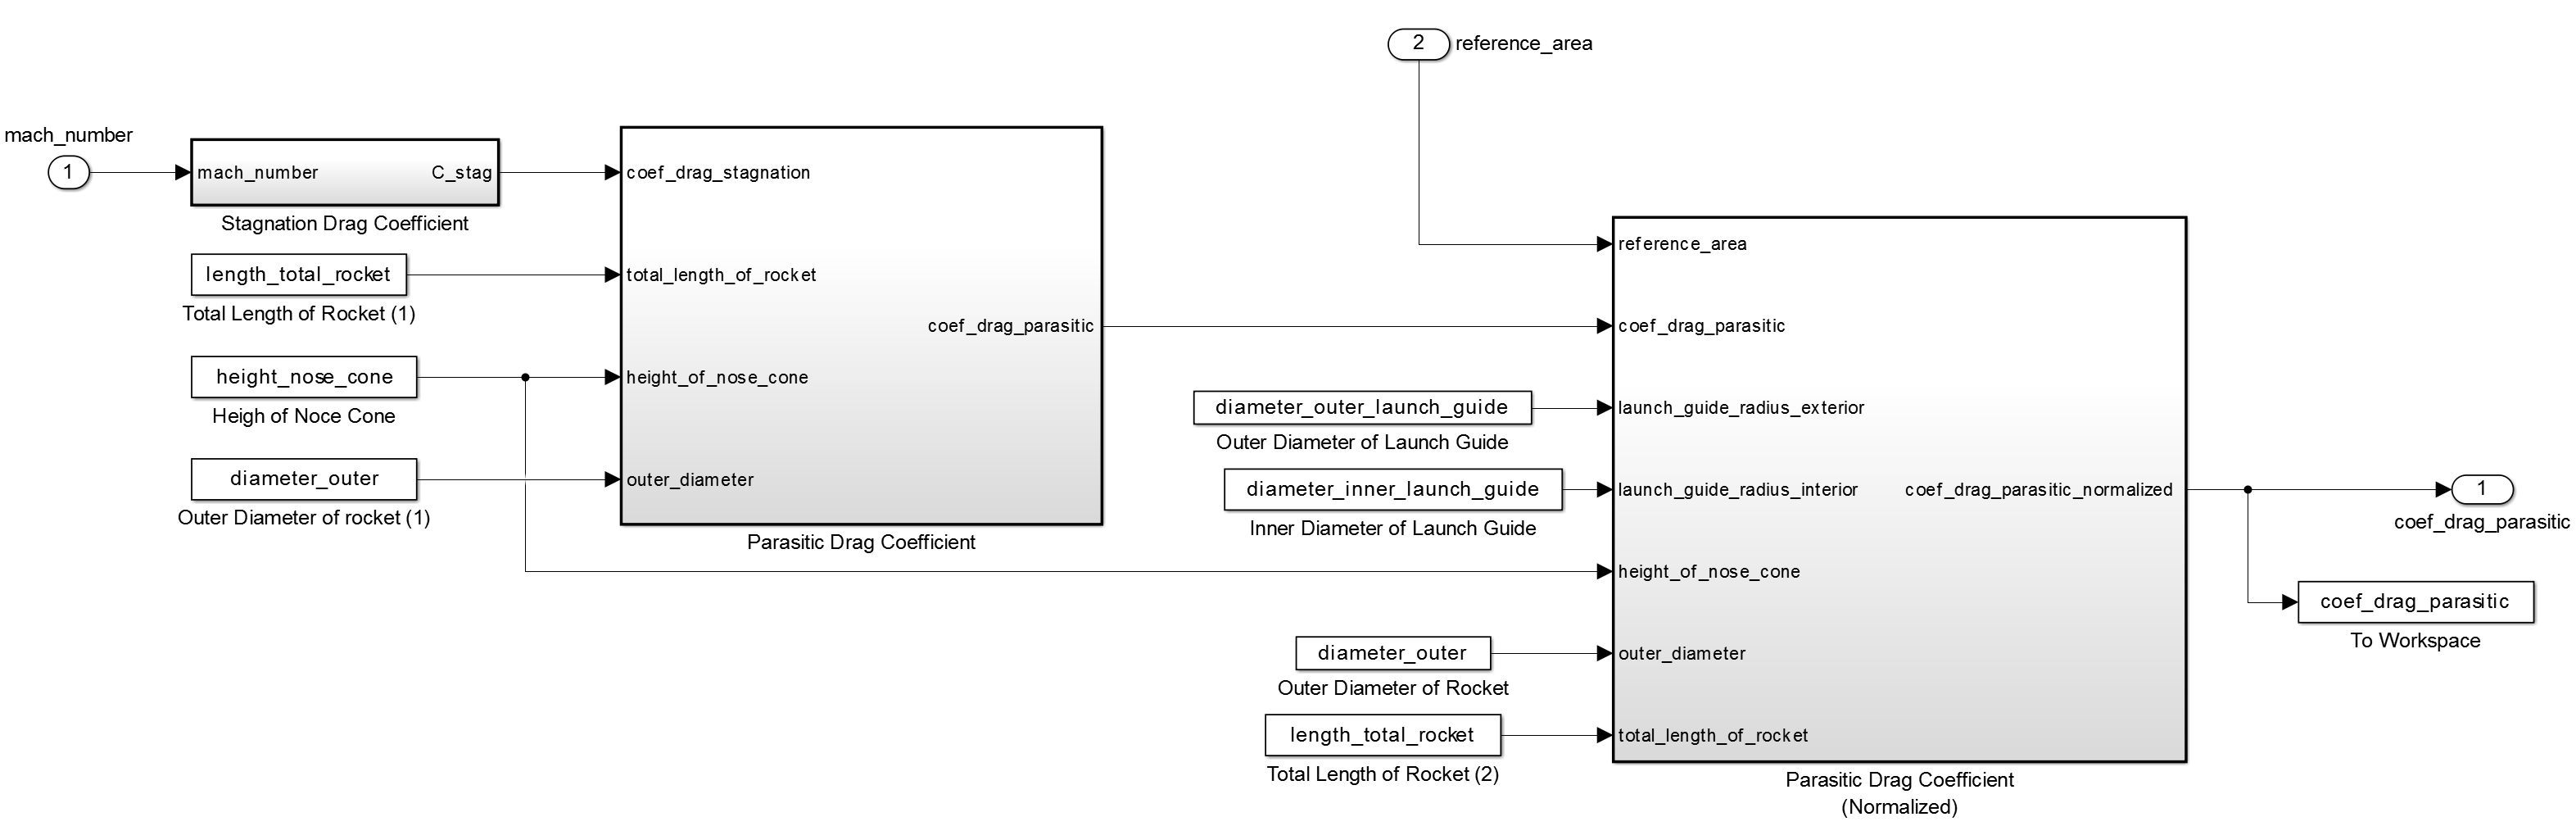
\includegraphics{images/drag/coef_drag_parasitic.png}
\caption{Matlab Implementation of Parasitic Drag
Coefficient\label{img_coef_drag_parasitic_label}}
\end{figure}

\subsubsection{Interference Drag}\label{interference-drag}

\emph{Interference Drag} is caused due to effects of air flow at the
interfaces of the fins and the body.

\begin{equation} 
C_{in}, D_{in} (A_{ref}, M) 
\end{equation}

\begin{equation}
\label{eq_interference_drag_coefficient}
C_{in} = 2 C_{sk,fins} \left( 1 + 2 \dfrac{T_f}{l_m} \right) \dfrac{4n(A_{f_p}-A_{f_e})} {\pi d^2_f}
\end{equation}

Where:

\begin{itemize}
\tightlist
\item
  \(C_{sk,fins}\) is the coefficient of skin friction (due to viscous
  effects) on the fins
\item
  \(n\) is the number of fins
\item
  \(A_{f_p}\) is the fin planform area

  \begin{equation}
  \label{eq_fin_planform_area}
  A_{f_p} = A_{f_e} + \dfrac{1}{2} d_f l_r
  \end{equation}
\item
  \(A_{f_e}\) is the exposed planform area of the fin

  \begin{equation}
  \label{eq_exposed_fin_planform_area}
  A_{f_e} = \dfrac{1}{2} (l_r + l_t) l_s 
  \end{equation}
\end{itemize}

{[}3{]}

Interference Drag effects are small in comparison to other drag effects
{[}4{]}, and are thus ignored at this stage of the project.

\subsection{Wave Drag}\label{wave-drag}

\emph{Wave drag} is drag associated with shock waves (independent of
viscous effects).

\begin{quote}
At transonic speed, shock waves form at the nose tip and at the leading
edge of the fins \ldots{} Momentum is transferred from the rocket to the
surrounding air via these shockwaves
\end{quote}

\subsection{Boat-Tail Drag}\label{boat-tail-drag}

A \emph{boat-tail} is a reduction in diameter of the body tube towards
the base of the rocket. Our rocket does not have a boat-tail, thus
\emph{Boat-Tail Drag} considerations are ignored.

\clearpage 

\section{Additional Drag at Angle of
Attack}\label{additional-drag-at-angle-of-attack}

When the rocket flies at a non-zero angle of attack, additional drag
considerations must be made. The reference area the rocket becomes
larger as the rocket is pitched into the free stream, exposing more of
the rocket body to pressure and stagnation effects.

In Figure \ref{rocket_drag_aoa_label}, velocity \(\vec{v}\) is the
apparent velocity of the center of pressure relative to the surrounding
air.

\begin{figure}[htbp]
\centering
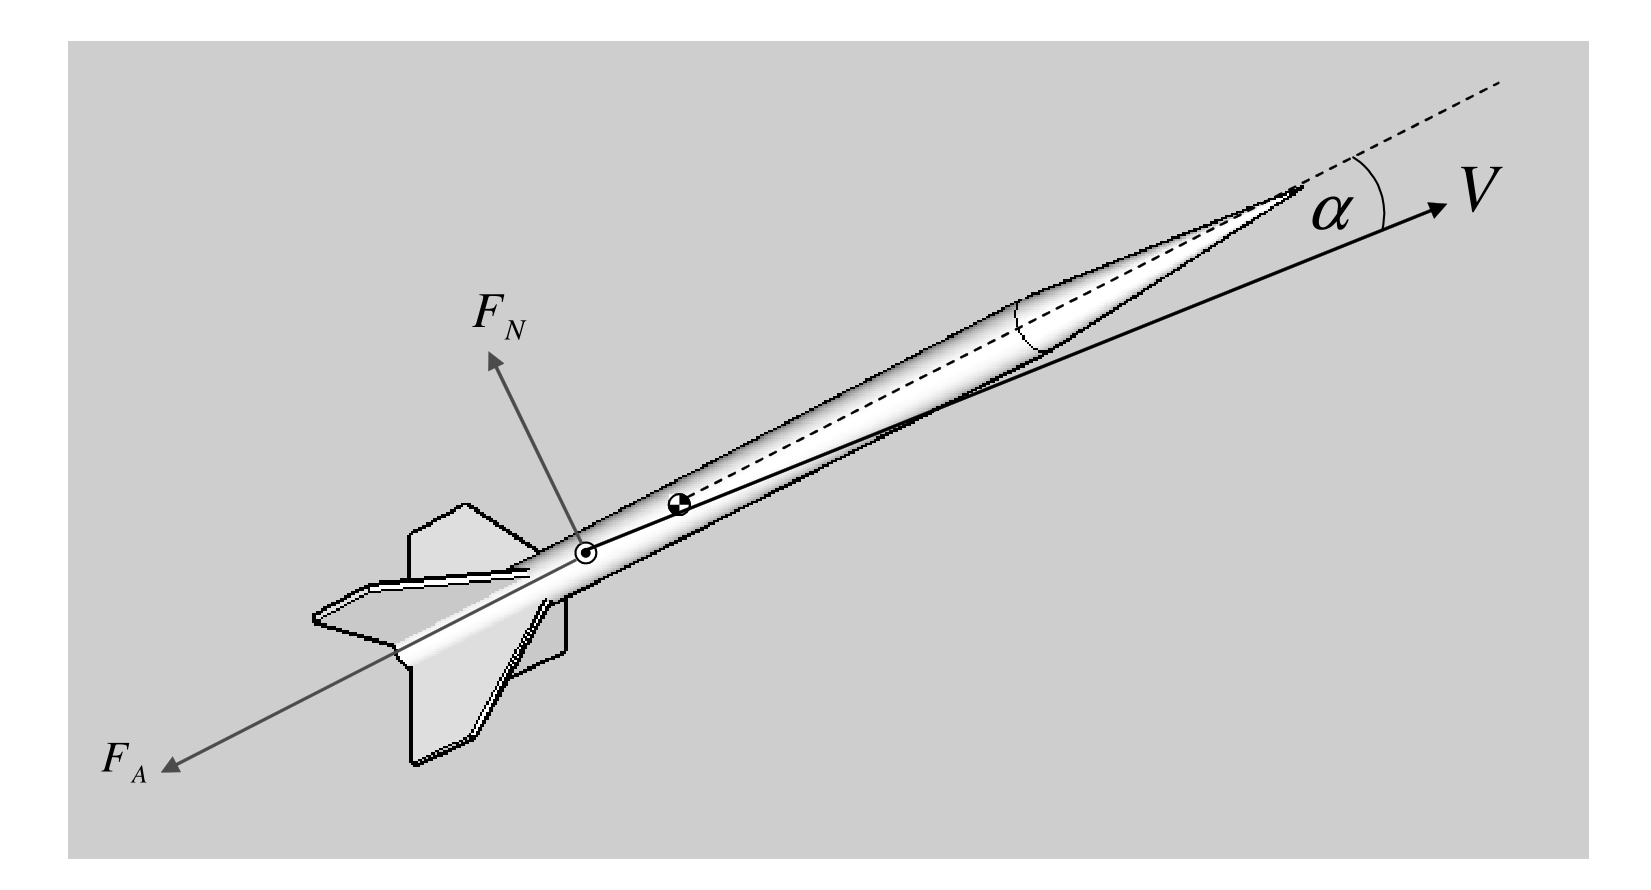
\includegraphics{images/rocket_drag_forces.png}
\caption{Rocket Drag Forces - Axial vs.~Normal Caption
\label{rocket_drag_aoa_label}}
\end{figure}

{[}3{]}

In the following analysis, additional rocket drag coefficients are
determined to be added to the \emph{zero angle of attack} drag
coefficient. This analysis is derived with the aid of additional
coefficients determined experimentally in wind tunnel tests on rocket
models {[}3{]} {[}2{]}.

\begin{equation}
\label{eq_rocket_drag_aoa}
C_{aoa} = C_{Db(\alpha)} + C_{Df(\alpha)}
\end{equation}

\subsection{Rocket Body Drag at Angle of
Attack}\label{rocket-body-drag-at-angle-of-attack}

\begin{equation}
\label{eq_rocket_body_drag_aoa}
C_{Db(\alpha)} = 2 \delta \alpha^2 + \dfrac{3.6 \eta (1.36 L - 0.55 h_n ) }{ \pi \cdot OD } \alpha^3
\end{equation}

Where:

\begin{itemize}
\tightlist
\item
  \(\alpha\) is the angle of attack
\item
  \(L\) is the total rocket length
\item
  \(OD\) is the outer diameter of the rocket
\item
  \(h_n\) is the height of the nose cone
\item
  \(\delta\) and \(\nu\) are experimentally determined coefficients
\item
  \(OD\) is the outer diameter of the rocket
\end{itemize}

{[}3{]}

\subsubsection{Rocket Fin Drag at Angle of
Attack}\label{rocket-fin-drag-at-angle-of-attack}

\begin{equation}
\label{eq_rocket_fin_drag_aoa}
C_{Df(\alpha)} = \alpha^2 \left[ 1.2 \dfrac{A_{fp}4}{\pi OD^2_f} + 3.12 (k_{fb} + k_{bf} - 1) \left( \dfrac{A_{fe} 4}{\pi OD^2_f} \right) \right]
\end{equation}

Where:

\begin{itemize}
\tightlist
\item
  \(k_{fb}\) is the fin-body coefficient

  \begin{equation}
  \label{eq_fin_body_coef_aoa}
  k_{fb} = 0.8065 R^2_s + 1.1553 R_s
  \end{equation}
\item
  \(k_{bf}\) is the body-fin coefficient

  \begin{equation}
  \label{eq_body_fin_coef_aoa}
  k_{bf} = 0.1935 R^2_s + 0.8174 R_s + 1
  \end{equation}
\item
  \(R_s\) is the fin section ratio

  \begin{equation}
  \label{eq_fin_section_ratio}
  R_s = \dfrac{l_{TS}}{d_f}
  \end{equation}
\item
  \(l_{TS}\) is the total span of the fins
\item
  \(OD_f\) is the diameter of the body tube at the base of the fin mount
\end{itemize}

{[}3{]}

\subsection{Alternatively}\label{alternatively}

{[}2{]} shares a function determined for \emph{Total drag coefficient
due to angle-of-attack}

\begin{equation}
\label{eq_darg_total_aoa}
C_d (\alpha) = 16.83 \alpha^2 + 8.9 \alpha^3
\end{equation}

\section{Matlab Implementation}\label{matlab-implementation}

Figure \ref{rocket_drag_model_label} below shows the \emph{Simulink}
implementation of the calculation of the drag model

\begin{figure}[htbp]
\centering
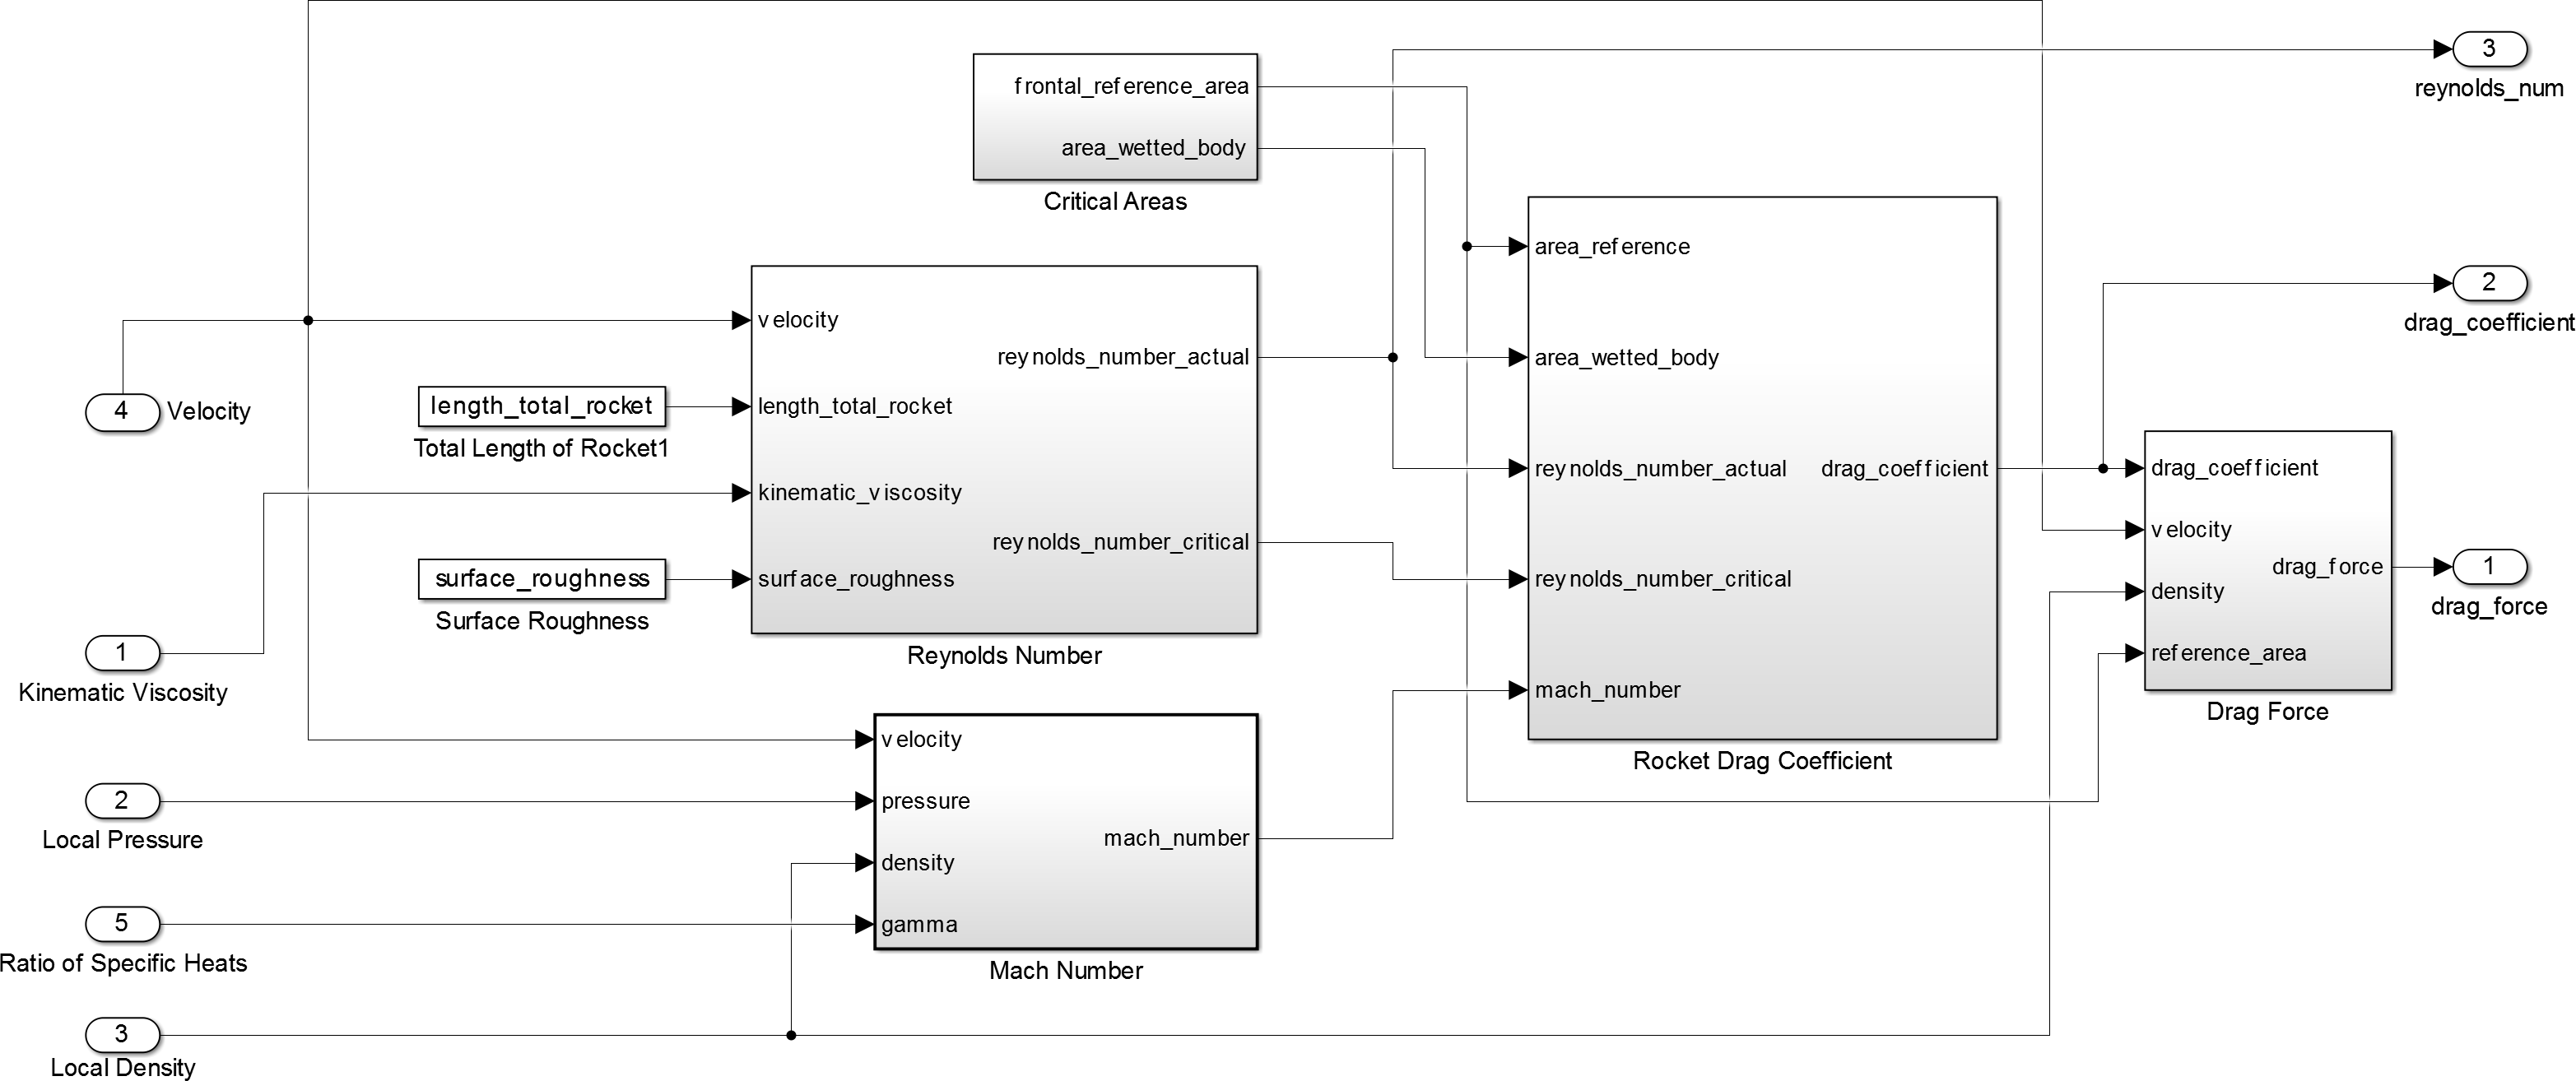
\includegraphics{images/rocket_drag_model.png}
\caption{Rocket Drag Model\label{rocket_drag_model_label}}
\end{figure}

\clearpage

Figure \ref{rocket_drag_coefficients_label} below shows the
\emph{Simulink} implementation of the calculation of drag coefficient

\begin{figure}[htbp]
\centering
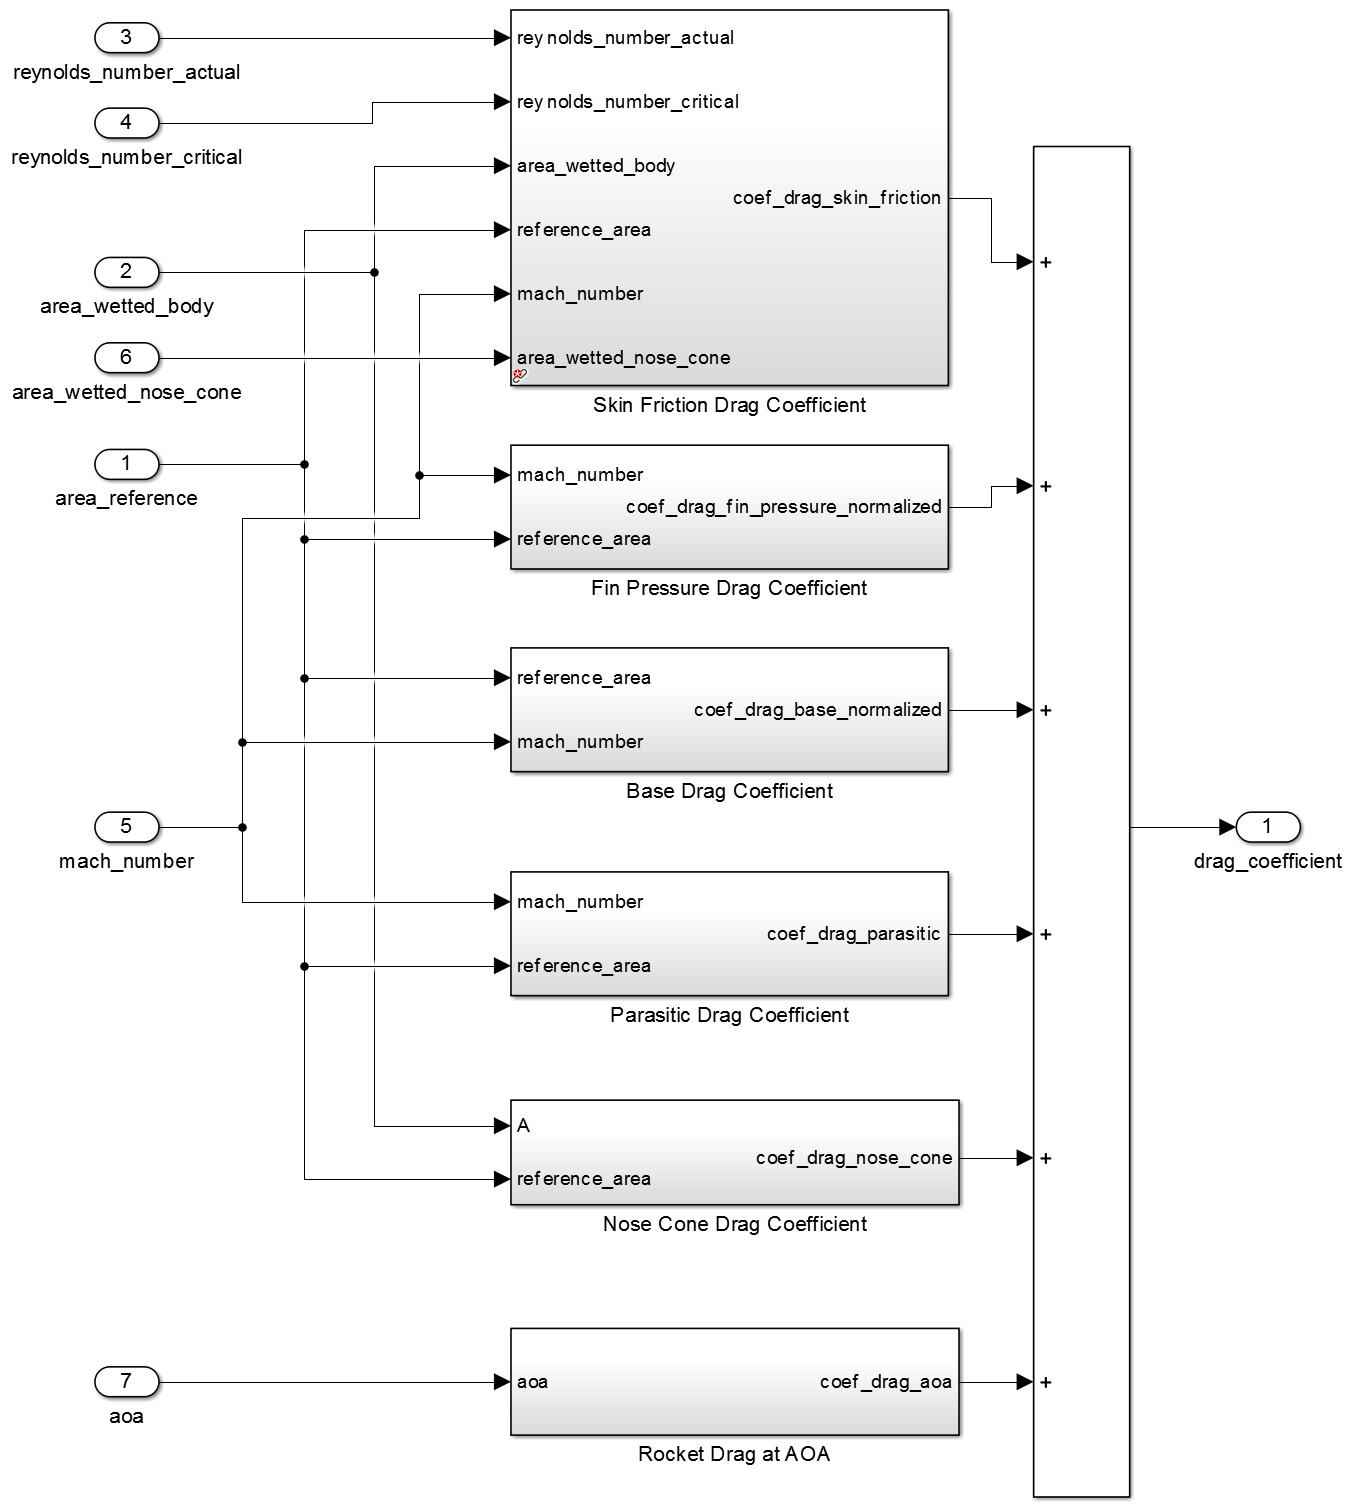
\includegraphics{images/rocket_drag_coefficient.png}
\caption{Rocket Drag Coefficient Model
\label{rocket_drag_coefficients_label}}
\end{figure}

\subsection{Matlab Validation}\label{matlab-validation}

The following plots show the Drag Model compared against OpenRocket,
RASAero, and Rocksim. The differences between the commercial simulations
are likely due to differing drag analysis methods which are not
available due to their closed source nature. However, it can be seen
that Matlab and OpenRocket are very close, which validates the Matlab
model since it was closely following the methods performed in OpenRocket

\begin{figure}[htbp]
\centering
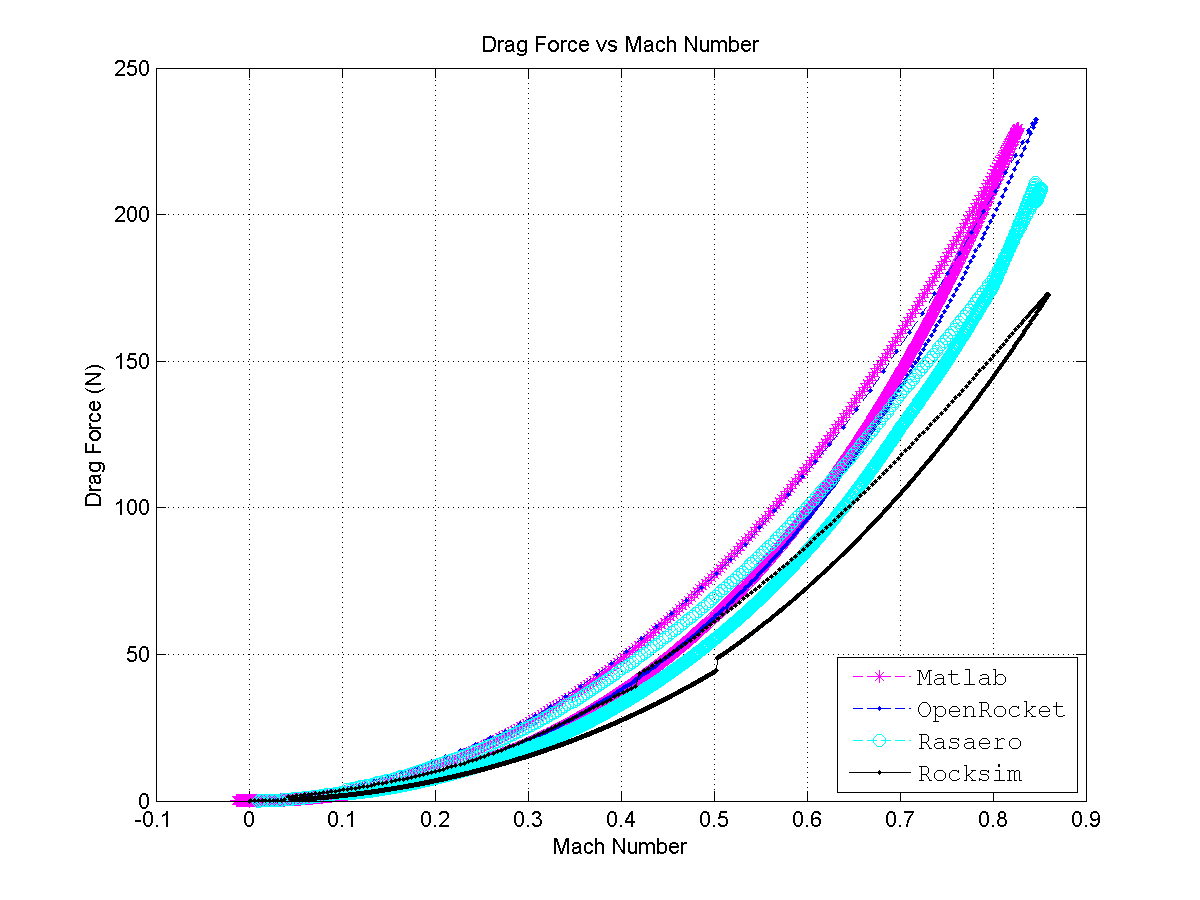
\includegraphics{images/plots/error_dragforce_plot.png}
\caption{Drag Force as a Function of Mach Number
\label{error_dragforce_v_plot_label}}
\end{figure}

\clearpage

\chapter{Point-Mass Flight Model}\label{point-mass-flight-model}

The analysis of the point-mass flight model can be simplified to a sum
of forces.

Simplifying the rocket flight as ideally one-dimensional, with the
positive z-direction being upwards from the launch pad, the impulse is
equal to the thrust of the rocket minus the weight of the rocket and the
drag forces of the rocket interacting with the surrounding air.

\begin{equation}
\label{eq_vertical_flight_eom}
m(t)\ddot{z}(t) = T(t) - D(\dot{z}) - W(t)
\end{equation}

Mass is a function of time, which is explained in the \emph{Dynamic
Parameters} section. Drag is a function of velocity, which is explained
in \emph{Drag Model} section. Acceleration can be expressed as the first
derivative of velocity and also the second derivative of position, each
with respect to time.

\begin{equation}
\vec{a} = \dot{v} = \ddot{z}
\end{equation}

Each force component can be rearranged and expressed as follows:

\begin{equation}
\vec{a}_T = \dfrac{T(t)}{m(t)}, \vec{a}_W = \dfrac{W(t)}{m(t)}, \vec{a}_D = \dfrac{D(v)}{m(t)}
\end{equation}

The net upward acceleration is: \(\vec{a}_T - \vec{a}_W - \vec{a}_D\)

The sum of forces can be rearranged and acceleration can be solved for:

\begin{equation}
\label{vertical_flight_equation}
\vec{a} =  \ddot{z} = \dfrac{1}{m(t)} (T(t) - D(\dot{z}) - W(t)) 
\end{equation}

Acceleration can be integrated to find position and velocity.

\begin{equation}
\vec{v} = \int \vec{a} dz
\end{equation}

\begin{equation}
z = \iint \vec{a} dz
\end{equation}

Integration of equation (\ref{vertical_flight_equation}) in the model is
represented by the \(\dfrac{1}{s}\) block. The model is pictured in
Figure \ref{vertical_model_simplified}.

\begin{figure}[htbp]
\centering
\includegraphics{images/vertical_model_simplified.png}
\caption{Vertical Flight Model - Simplified
\label{vertical_model_simplified}}
\end{figure}

\section{Weathercocking}\label{weathercocking}

\emph{Weathercocking} is a phenomenon when the rocket tends to alter its
trajectory and fly into the wind. If the rocket is stable, and has a
sufficiently high damping ratio, the rocket eventually reaches a
near-zero angle-of-attack parallel to the velocity vector of the wind,
only in the opposite direction.

If we apply a wind velocity in the drag calculation, we can then modify
Equation \ref{eq_vertical_flight_eom} to account for weathercocking and
provide the actual altitude reached, as well as the amount of drift
experienced.

\section{Altitude accounting for flight
angle}\label{altitude-accounting-for-flight-angle}

\begin{equation}
\label{eq_vertical_angle}
m(t)\ddot{z}(t) = T(t) \cos \theta - D(\dot{z}) \cos \theta - W(t)
\end{equation}

Where:

\begin{itemize}
\tightlist
\item
  \(z\) is the upward direction (normal from the ground)
\item
  \(\theta\) is the angle between the current rocket trajectory and the
  z-axis
\end{itemize}

\section{Drift accounting for flight
angle}\label{drift-accounting-for-flight-angle}

\begin{equation}
\label{eq_vertical_angle}
m(t) \ddot{z}(t) = T(t) \sin \theta - D(\dot{z}) \sin \theta 
\end{equation}

\chapter{Rigid-Body Rotation (Pitch, Yaw) Stability
Analysis}\label{rigid-body-rotation-pitch-yaw-stability-analysis}

\section{Overview}\label{overview-2}

Due to disturbances such as wind, and imperfections and imbalances in
the construction, the rocket will tend to fly at an \emph{Angle of
Attack} into the free stream, wherein the velocity vector (taken from
the \emph{Center of Gravity}) is not parallel with the longitudinal
axis. This will cause non-linear changes to the magnitude of the
aerodynamic forces, which, as a further simplification, can be said to
be acting on the \emph{Center of Pressure}. In order for the aerodynamic
forces to straighten the rocket in its forward motion, and to stabilize
the oscillatory rotation about the COG, the COP must be located behind
the COG.

The moment arm about the COG is the distance of the COP from the tip of
the nose cone, minus the distance of the COG from the tip of the nose
cone. Then, the sum of forces at the COP is the \emph{Restoring Force}
(\(F_R\)) minus the \emph{Damping Force} (\(F_D\)), and the sum of the
Moments about the COG is expressed as follows.

The \emph{Moment} of a rigid body about its COG can be expressed as the
product of the \emph{Moment of Inertia} of the rigid body and the
\emph{Angular acceleration} of the body.

\begin{equation}
\label{eq_moment}
M = I \lambda 
\end{equation}

\begin{itemize}
\tightlist
\item
  \(\lambda\) is the \emph{angular acceleration} of the rigid body,
  which is the second time derivative of the angular displacement
\end{itemize}

\[ 
\lambda = \ddot{\alpha}
\] \[
\omega = \dot{\alpha}
\]

\begin{itemize}
\tightlist
\item
  \(\omega\) is the \emph{angular velocity}, which is the first time
  derivative of the angular displacement
\item
  \(\alpha\) is the \emph{angle of attack}
\end{itemize}

\section{Longitudinal Static Stability
Margin}\label{longitudinal-static-stability-margin}

The \emph{Longitudinal Static Stability Margin} (\(S_{lm}\)) is the
distance between the \emph{Center of Gravity} and the \emph{Center of
Pressure} divided by the outer diameter of the body tube when the rocket
is positioned at an angle-of-attack (\(\alpha\)) of zero {[}2{]}.

\[ S_{lm} = \dfrac{COP - COG}{OD} \]

When traveling under a non-zero angle of attack, the Stability Margin is
adjusted using the body lift correction factor Equation
\ref{eq_coefficient_normal_force_body_lift}.

The result is dimensionless, however the ratio determined is measured in
the number of \emph{calibers}.

\begin{quote}
2a - The static stability margin falls above 2 (but less than 3)
calibers at launch
\end{quote}

\section{Requirement}\label{requirement}

\begin{itemize}
\tightlist
\item
  2a - The static stability margin falls above 2 (but less than 3)
  calibers at launch
\item
  2b - The dynamic stability is greater than 0 even in winds up to 8.33
  m/s
\item
  2f - The vehicle does not experience resonant pitching/yawing motion
  in flight
\end{itemize}

\section{Assumptions}\label{assumptions-2}

\begin{itemize}
\tightlist
\item
  small angle of attack (less than 10\(^\circ\))
\item
  incompressible flow
\item
  neglect viscous forces
\item
  neglect compressibility effects {[}3{]}
\item
  neglect lift force on the body tube {[}3{]}
\item
  neglect the effect of roll due to having 3 fins vs 4
\end{itemize}

\section{Definition of Terms}\label{definition-of-terms}

\subsection{Rocket Normal Force}\label{rocket-normal-force}

The \emph{Rocket Normal Force} is the resultant force applied at the
\emph{Center of Pressure} perpendicular to the longitudinal axis of the
rocket, when the rocket flies at an angle-of-attack.

\begin{equation}
\label{rocket_normal_force}
F_{N} = \dfrac{1}{2} \rho \vec{v}^2 A_{c} C_N
\end{equation}

{[}3{]}

Where \(A_c\) is the cross-sectional area of the body tube, and \(C_N\)
is the \emph{Normal Force Coefficient}, and is a function of
angle-of-attack (\(\alpha\)). The small angle approximation is applied,
wherein small angles can be approximated as a linear function of the
angle.

\begin{equation}
\label{normal_force_coefficient}
C_N = C_{N \alpha} \cdot \alpha
\end{equation}

{[}3{]}

\subsection{Corrective Moment
Coefficient}\label{corrective-moment-coefficient}

The \emph{Corrective Moment Coefficient} describes the reaction of the
rocket against a disturbance about its longitudinal axis.

\begin{equation}
\label{eq_coef_moment_corrective}
C_{MC} = \dfrac{1}{2} \rho \vec{v}^2 A_{ref} C_{N \alpha} (COP-COG)
\end{equation}

Where:

\begin{itemize}
\tightlist
\item
  \(\rho\) is the local density of air
\item
  \(\vec{v}\) is the velocity of the rocket
\item
  \(A_{ref}\) is the reference area of the rocket flying into the free
  stream
\item
  \(C_{N \alpha}\) is the \emph{Stability Derivative} \sout{\emph{Normal
  Force Coefficient}}
\item
  \((COP-COG)\) is the distance between the \emph{Center of Pressure}
  and \emph{Center of Gravity}
\end{itemize}

Note: a rocket with a high \emph{Corrective Moment Coefficient} is going
to weathercock faster at lower velocities.

\href{https://www.apogeerockets.com/education/downloads/Newsletter193.pdf}{Corrective
Moment Coefficient}

\subsubsection{Dimensional Analysis}\label{dimensional-analysis}

\begin{equation}
\label{eq_c1_dim_anal}
\dfrac{kg}{m^3} \left[ \dfrac{m}{s} \right]^2 m^2 m = \dfrac{kg \cdot m }{s^2} \cdot m 
\end{equation}

\subsection{Damping Moment
Coefficient}\label{damping-moment-coefficient}

As the rocket responds to a disturbance, the \emph{Corrective Moment}
reactions forces act in an oscillating manner - weathercocking into the
wind, then turning back towards the vertical direction. In order to
reach dynamic stability, this oscillation must decay and settle to a
reasonable response. The \emph{Damping Moment Coefficient} represents
how fast the response settles towards zero.

There are two \emph{Damping Moment Coefficients} to consider, the
\emph{Aerodynamic Damping Moment Coefficient} and the \emph{Propulsive
Damping Moment Coefficient}.

Then the \emph{Damping Moment Coefficient} is the sum of the two moment
components coefficients.

\begin{equation}
\label{eq_coef_moment_damping}
C_{DM} = C_{ADM} + C_{PDM}
\end{equation}

\subsubsection{Aerodynamic Damping Moment
Coefficient}\label{aerodynamic-damping-moment-coefficient}

Each rocket component contributes to the \emph{Aerodynamic Damping
Moment Coefficient}

\begin{equation}
\label{eq_coef_moment_damping_aero}
C_{ADM} = \dfrac{1}{2} \rho \vec{v} A_{ref} \sum \left( C_{N \alpha,x} \cdot \left[ COP_{x} - COG \right]^2  \right) 
\end{equation}

NOTE: Why isn't \(\vec{v}\) SQUARED? It might have something to with the
fact that the ADM is a function of angular displacement, and DM is a
function of angular velocity??

Where:

\begin{itemize}
\tightlist
\item
  \(\rho\) is the local density of air
\item
  \(\vec{v}\) is the velocity of the rocket
\item
  \(A_{ref}\) is the reference area of the rocket flying into the free
  stream
\item
  \sout{\(C_{NF,x}\)} \(C_{N \alpha}\) is the \sout{\emph{Normal Force
  Coefficient}} \emph{Stability Derivative}
\item
  \(COP_{x}\) is the distance of \emph{Center of Pressure} of the rocket
  component to the nose cone tip
\item
  \(COG\) is the distance between the rocket \emph{Center of Gravity} to
  the nose cone tip
\end{itemize}

\paragraph{Dimensional Analysis}\label{dimensional-analysis-1}

\begin{equation}
\label{eq_c2a_dim_anal}
\dfrac{kg}{m^3} \dfrac{m}{s} m^2 m^2 = \dfrac{kg \cdot m }{s} \cdot m 
\end{equation}

\subsubsection{Propulsive Damping Moment
Coefficient}\label{propulsive-damping-moment-coefficient}

Also known as \emph{Jet Damping}, as propulsion creates forward
momentum, it resists rotation of the rocket.

\begin{equation}
\label{eq_coef_moment_damping_jet}
C_{PDM} = \dot{m} \left( d_{tip,nozzle} - COG \right) ^2
\end{equation}

\paragraph{Jet Damping - Dimensional
Analysis}\label{jet-damping---dimensional-analysis}

\[
\dot{m} \left( d_{tip,nozzle} - COG \right) ^2 :
\left[ \dfrac{kg}{s} \cdot m^2 \right]
\] \[
M = fd : 
\left[ \dfrac{kg \cdot m^2}{s^2} \right]
\]

Note: why is the \emph{Jet Damping Moment} missing a 1/t?

\href{https://www.apogeerockets.com/education/downloads/Newsletter195.pdf}{Damping
Moment Coefficient - Source}

\subsubsection{Pitch Damping Moment}\label{pitch-damping-moment}

The \emph{Pitch Damping Moment} is a moment opposing the \emph{Rocket
Restoring Moment} and dampens the oscillation.

\begin{equation}
\label{eq_moment_damping_pitch}
0.55 \dfrac{l^4 r_t}{A_{ref} d} \dfrac{\omega^2}{v^2_0}
\end{equation}

According to {[}4{]}, the \emph{Pitch Damping Moment} is essentially
insignificant until near apogee. This is because it is proportional to
\(\dfrac{\omega^2}{v^2_0}\) (as seen in \ref{eq_moment_damping_pitch}),
which will be near zero until apogee due to very small angular
velocities made smaller by squaring the \(\omega\) term.

The \emph{Pitch Damping Moment} of each rocket component must be
calculated individually. For instance, the \emph{Pitch Damping Moment}
of a fin is as follows.

\begin{equation}
\label{eq_moment_damping_pitch_fin}
C_{damp} = 0.6 \dfrac{N A_{fin} d_{COP}^3}{A_{ref} d} \dfrac{\omega^2}{v^2_0}
\end{equation}

\section{Derivation of the Harmonic Motion
Equation}\label{derivation-of-the-harmonic-motion-equation}

Suppose a high-powered rocket is launched in quiescent air vertically,
and flies straight without wobbling. Then, suppose a small and momentary
disturbance (e.g.~a short gust of wind) is experienced on the side of
the rocket causing an angular deflection, . If the rocket is
\emph{stable}, a restoring force causes a \emph{corrective moment} which
will act in the opposite direction of the deflection. This
\emph{corrective moment} can be considered a function of angular
displacement {[}2{]}.

\begin{equation}
M_{corrective} = F (\alpha)
\end{equation}

As the rocket gains velocity in the direction opposite the disturbance,
a \emph{damping moment} is generated as a result of the relative speed
of the air, in the direction orthogonal to the longitudinal axis. As
this \emph{damping moment} opposes the angular velocity caused by the
\emph{corrective moment}, its sign is opposite to the angular velocity.
The \emph{damping moment} is also a function of angular velocity
{[}2{]}.

\begin{equation}
M_{damping} = G (\omega)
\end{equation}

Then, taking a sum of Moments, the rotation of the rocket can be
described as follows {[}2{]}

\[
I \lambda = -F(\alpha) - G(\omega) 
\] \[
I \left( \dfrac{d^2\alpha}{dt^2} \right) = -F(\alpha) - G \left(\dfrac{d\alpha}{dt} \right) 
\]

\begin{equation}
\label{eq_rocket_diff}
I \left( \dfrac{d^2\alpha}{dt^2} \right) + F(\alpha) + G \left(\dfrac{d\alpha}{dt} \right) = 0
\end{equation}

This nonlinear, homogenous, differential equation can not be solved
exactly {[}2{]}.

\section{Linearization Approximation}\label{linearization-approximation}

Linear Approximations of \ref{eq_rocket_diff} are made considering small
values of \(\alpha\) and \(\omega\), known as the
\emph{small-perturbation theory} {[}2{]}. This linearization process
provides \sout{constant} coefficients, which we will denote \(C_1\) for
the \emph{Corrective Moment Coefficient} and \(C_2\) for the
\emph{Damping Moment Coefficient}.

\[
F(\alpha) \approx C_1 \cdot \alpha 
\] \[
G \left(\dfrac{d\alpha}{dt} \right) \approx C_2 \cdot \dfrac{d\alpha}{dt} 
\]

\begin{equation}
\label{eq_rocket_diff_linearized}
I \left( \dfrac{d^2\alpha}{dt^2} \right) + C_1 (\alpha) + C_2 \left(\dfrac{d\alpha}{dt} \right) = 0
\end{equation}

\section{General Homogeneous
Response}\label{general-homogeneous-response}

The characteristic, linearized, homogeneous yaw/pitch response is given
as:

\begin{equation}
I_L \dfrac{d^2 \alpha_x}{dt^2} + C_2 \dfrac{d \alpha_x}{dt} + C_1 \alpha_x = 0
\end{equation}

{[}2{]}

A solution over a known range of acceptable values of the coefficients
above is:

\begin{equation}
\label{eq_yaw_pitch_time_response}
\alpha_x = A e^{-Dt} \sin(\omega t + \phi)
\end{equation}

Where:

\begin{itemize}
\tightlist
\item
  \(t\) is the time passed since the ``observation of the dynamic
  response has begun, not the time elapsed since the rocket was
  launched'' {[}2{]}
\item
  \(\omega\) is the \emph{frequency of oscillation} (not literally the
  angular velocity of the rocket)
\end{itemize}

\begin{equation}
\label{eq_frequency_oscillation}
\omega = \sqrt{ \dfrac{C_1}{I_L} - \dfrac{C_2^2}{4 I_L^2} }
\end{equation}

\begin{itemize}
\tightlist
\item
  \(\phi\) is the \emph{phase angle} in radians

  \begin{equation}
  \label{eq_phase}
  \phi = 
  \arctan { 
  \left( \dfrac{ \alpha_{xo} \omega } { D\alpha_{xo} + \Omega_{xo} } \right) 
  }
  \end{equation}
\item
  \(D\) is the \emph{inverse time constant}

  \begin{equation}
  \label{eq_inverse_time_constant}
  D = { C_2 \over 2 I_L }
  \end{equation}
\item
  \(A\) is the \emph{initial amplitude}

  \begin{equation}
  A = \dfrac{\alpha_{xo}}{sin \phi}
  \end{equation}
\item
  \(\alpha_{xo}\) is the value of \(\alpha_x\) at \(t=0\)
\end{itemize}

{[}2{]}

The initial conditions for this solution are

\begin{itemize}
\tightlist
\item
  \(a_{xo}\) = some non-zero angle-of-attack
\item
  \(\Omega_{xo}\) = 0
\end{itemize}

This equation is represented in the model as follows

\begin{figure}[htbp]
\centering
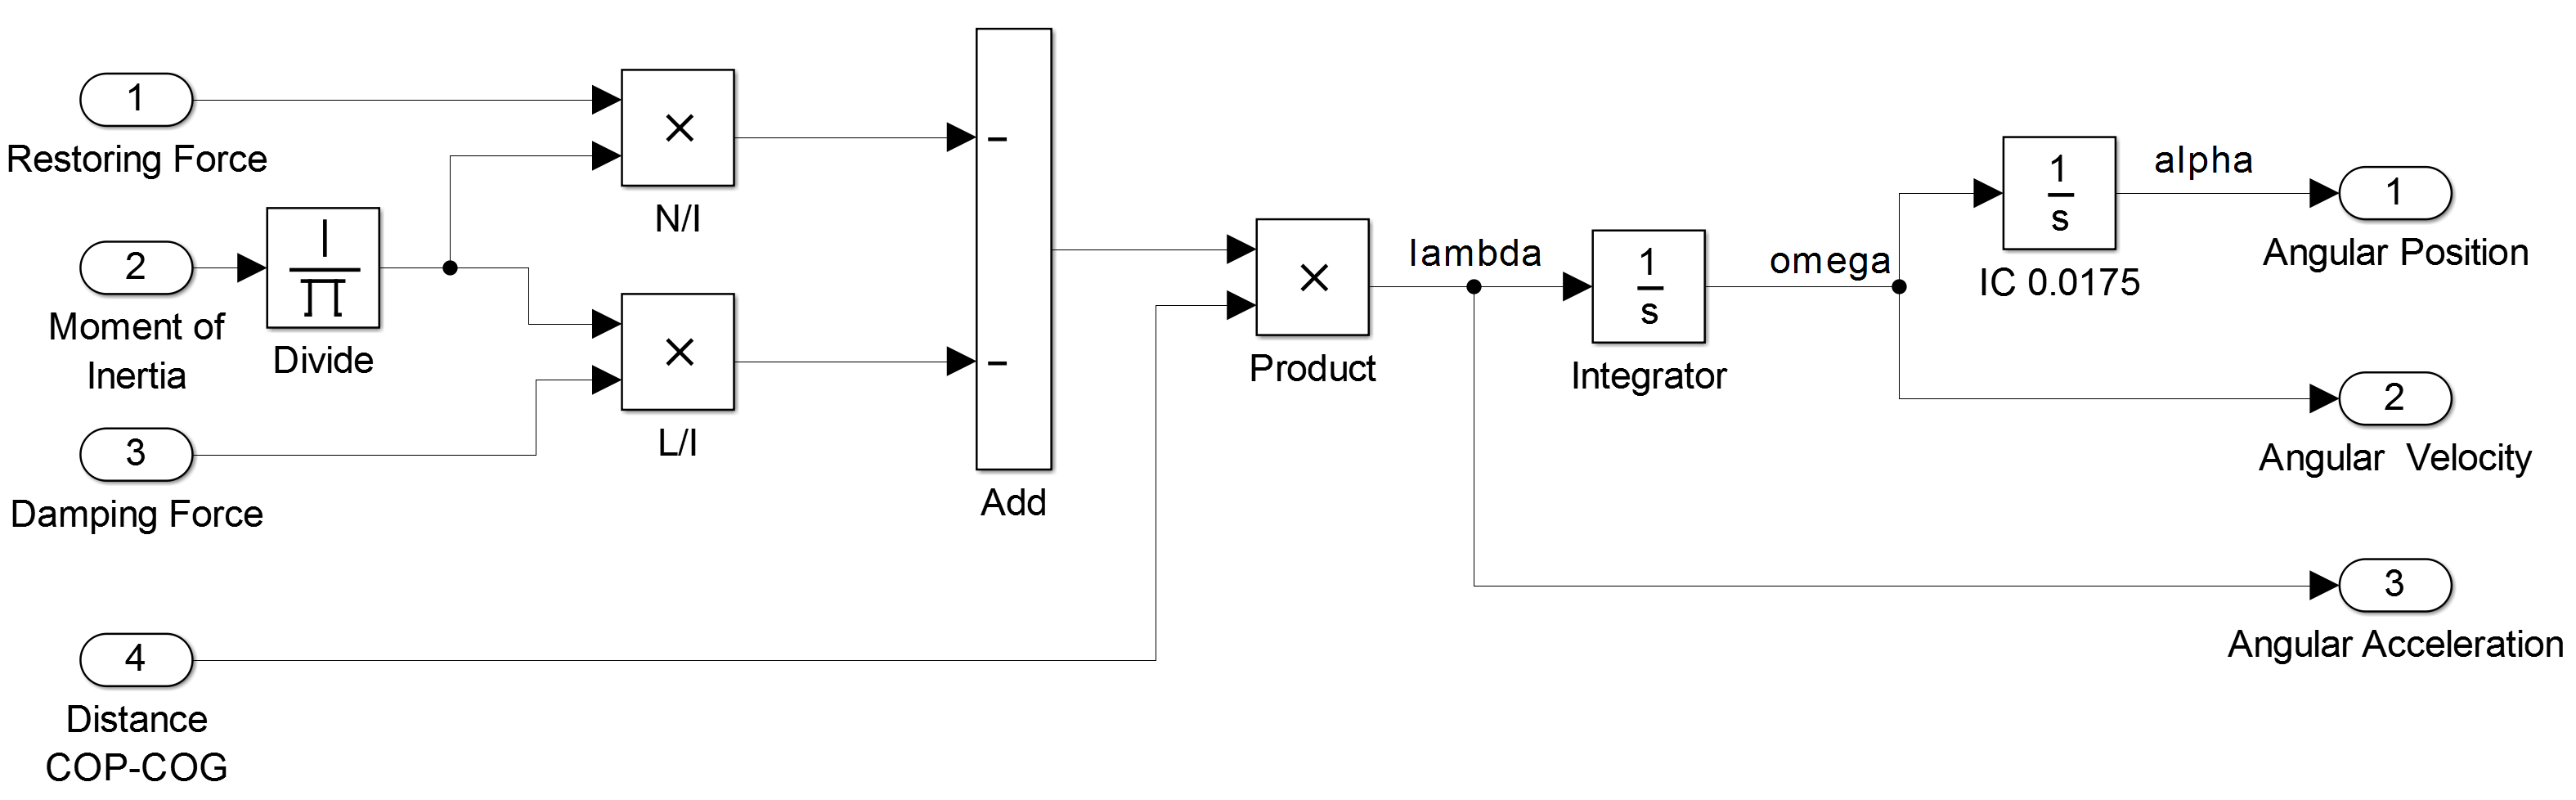
\includegraphics{images/angular_model_simplified.png}
\caption{Angular Flight Model - Simplified
\label{angular_model_simplified}}
\end{figure}

\[
I_L (D^2 - \omega^2) - C_2 D + C_1 = 0
\] \[
-2 I_L D + C_2 = 0
\]

{[}2{]}

A rocket can be considered restored from a disturbance if the angle of
attack decays to 5\% of the initial amplitude {[}2{]}.

{[}2{]}

The \emph{Natural Frequency} of the rocket at the current air speed for
the homogeneous solution is

\begin{equation}
\label{eq_natural_frequency_homogeneous}
\omega_n = \sqrt{ \dfrac{C_1}{I_L} }
\end{equation}

Note: it would appear that this response only reflects the physical
system for non-decreasing values of \(C_2\), which would cause the
exponential term to increase with time and cause the amplitude to grow.
Although the damping coefficient remains relatively constant, the
inverse time-constant is only a function of \(\dfrac{C_2}{2 I_L}\). As
velocity decreases in the rocket coasting phase, \(C_2\) drops
proportional to the square of the velocity and thus the inverse-time
constant decreases enough with respecting time, that \(Dt\) is
decreasing and thus \(e^{-Dt}\) will begin to increase. This is
accounted for by the drift velocity at apogee. While the rocket has a
zero climbing velocity, it does still travel laterally and the total
velocity contributes to the damping moment coefficient, maintaining
stability.

\section{Complete Response to Step
Input}\label{complete-response-to-step-input}

\section{Complete Response to Impulse
Input}\label{complete-response-to-impulse-input}

\subsection{Delta-Dirac Function}\label{delta-dirac-function}

\begin{equation}
\label{eq_delta_dirac}
u(t) = \int_{-\infty}^{\infty} \delta ( u - \tau ) d \tau
\end{equation}

\subsection{Convolution Theorem}\label{convolution-theorem}

\section{Steady State Response to Sinusoidal
Forcing}\label{steady-state-response-to-sinusoidal-forcing}

\subsection{Rocket Damping Ratio}\label{rocket-damping-ratio}

The \emph{Rocket Damping Ratio} is calculated as follows.

\begin{equation}
\label{eq_rocket_damping_ratio}
\zeta = \dfrac{C_2}{2 \cdot \sqrt{C_1 I_L}}
\end{equation}

Where:

\begin{itemize}
\tightlist
\item
  \(C_1\) is the \emph{Corrective Moment Coefficient}
\item
  \(C_2\) is the \emph{Damping Moment Coefficient}
\item
  \(I_L\) is the \emph{Longitudinal Moment of Inertia}
\end{itemize}

{[}2{]}

\subsubsection{Underdamped Case}\label{underdamped-case}

\begin{equation}
0 < \dfrac{C_2^2}{4I_L^2} < \dfrac{C_1}{I_l} \
\end{equation}

The fastest response is when \(\zeta = \dfrac{\sqrt{2}}{2}\)

\subsubsection{Overdamped Case}\label{overdamped-case}

\begin{equation}
\dfrac{C_2^2}{4I_L^2} > \dfrac{C_1}{I_l} \
\end{equation}

\subsubsection{Critically Damped Case}\label{critically-damped-case}

\begin{equation}
\dfrac{C_1}{I_l} = \dfrac{C_2^2}{4I_L^2}
\end{equation}

{[}2{]}

\subsection{Rocket Natural Frequency}\label{rocket-natural-frequency}

\begin{equation}
\label{rocket_natrual_frequency}
\omega_n = \sqrt{\dfrac{C_1}{I_L}}
\end{equation}

Where:

\begin{itemize}
\tightlist
\item
  \(C_1\) is the \emph{Corrective Moment Coefficient}
\item
  \(I_L\) is the \emph{Longitudinal Moment of Inertia}
\end{itemize}

{[}2{]}

\subsection{Time Constants of the
Response}\label{time-constants-of-the-response}

\subsection{Complete response to step
input}\label{complete-response-to-step-input-1}

\subsection{Complete response to impulse
input}\label{complete-response-to-impulse-input-1}

{[}2{]}

\subsection{AOA as a function of
velocity}\label{aoa-as-a-function-of-velocity}

In order to plot the real system behavior, it may be possible to solve
Equation \ref{eq_rocket_diff} where \(\alpha_x\) is a function of
velocity, and solve for \(\alpha_x\) by twice integrating
\(\ddot{\alpha_x}\).

Since AOA is a function of total velocity through the \emph{Corrective
Moment Coefficient} and the \emph{Damping Moment Coefficient}, it may be
possible to solve the system by differentiating with respect to
velocity, rather than by time.

\[
I \left( \dfrac{d^2\alpha}{dt^2} \right) + F(\alpha) + G \left(\dfrac{d\alpha}{dt} \right) = 0
\]

\[
\dfrac{\delta^2 \alpha_x}{\delta t^2} = \dot{v} = \ddot{x}
\]

\[
\dfrac{\delta \alpha_x}{\delta t} = v = \dot{x}
\]

\[
\dfrac{\delta \alpha_x}{\delta t} = v = \dot{x}
\]

Somehow get to:

\[
\dfrac{d^2}{dv^2} ...
\]

\subsection{Corrections}\label{corrections}

\subsubsection{Compressibility
Correction}\label{compressibility-correction}

\emph{Barrowman's Method} neglects compressibility effects, however
these effects cannot be neglected above Mach 0.3.

\section{Wind Disturbance}\label{wind-disturbance}

We are interested in the damping ratio of the rocket as it stabilizes
towards \emph{zero angle of attack} in reaction to angular disturbances.

As we consider the rocket to have ideal dimensional accuracy, the main
source of flight disturbance is wind.

\subsection{Impulse Disturbance}\label{impulse-disturbance}

We can test the ability of the rocket to stabilize due to an initial
angular disturbance, by applying an initial angle of attack. This
simulates a small gust of wind hitting the rocket just as it takes off.

\subsection{Constant Disturbance}\label{constant-disturbance}

We can test the ability of the rocket to stabilize due to a constant
disturbance force, as well as applying an initial \emph{angle of
attack}. This simulates a constant wind force coming from a single
direction. As the density of air goes down with increases altitude, this
assumes that the wind speed picks up at higher altitudes to maintain the
constant wind force.

Alternatively, we could model a constant wind speed of \(8.33 m/s\), and
apply the ISA Model for the density as a function of altitude to
determine the changing wind force as the rocket climbs.

\section{More Reading}\label{more-reading}

There are further resources on rocket flight stability here: -
http://www.apogeerockets.com/Tech/Rocket\_Stability

\section{Solver Algorithm}\label{solver-algorithm}

The numerical algorithm chosen for performing the simulation can impact
the accuracy of the results. The following discussion introduces
available algorithms and their tradeoffs.

\subsection{Algorithms}\label{algorithms}

\subsubsection{Interpolation}\label{interpolation}

\paragraph{Matlab Cubic Spline}\label{matlab-cubic-spline}

\subsubsection{}\label{section}

\subsection{Runge-Kutta-Fehlberg}\label{runge-kutta-fehlberg}

Integration method order: Integration step size: Convergence Tolerance

\chapter{Validation}\label{validation-1}

The engineering flight simulation was tested comprehensively.

\section{Unit Testing}\label{unit-testing}

It was ensured that individual Matlab functions provided the output
expected, and that Simulink blocks employing the Matlab functions worked
on a unit level - Reference Models were employed for this purpose

\section{Integration Testing}\label{integration-testing}

\begin{figure}[htbp]
\centering
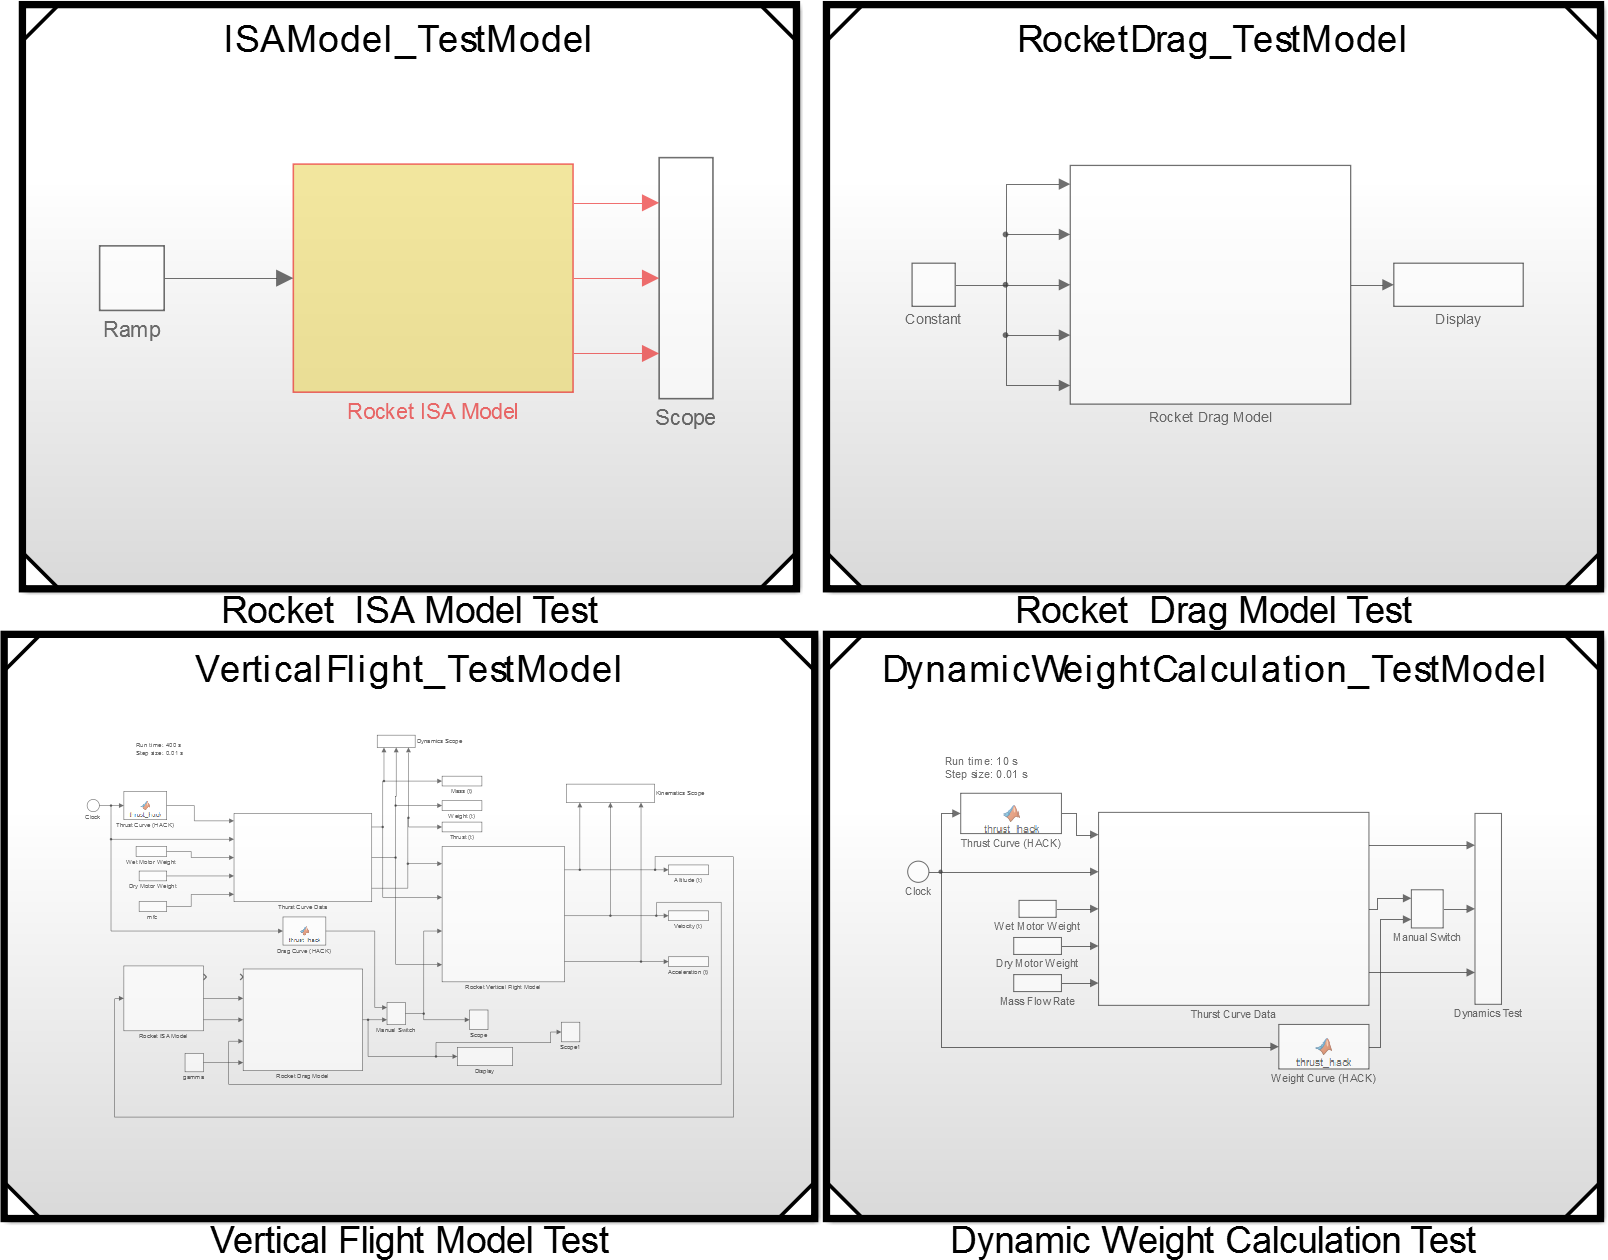
\includegraphics{images/ALL_TESTS.png}
\caption{All Integration Tests \label{all_integration_tests_label}}
\end{figure}

\clearpage

\section{System Testing}\label{system-testing}

The simulator was tested on a system level by simulating the CR\_2-4G
rocket flight on all available simulators and comparing all possible
results. These results are discussed in detail in the \emph{Simulation
Execution} section.

\chapter{Comparison with Experimental
Data}\label{comparison-with-experimental-data}

So far, much of the analysis has relied on theory and comparison with
other simulator output. It is important to compare our models with real
data to provide the best measure of their accuracy. Without access to a
wind tunnel, we determined that we could test our \emph{ISA Model}
implementation against weather balloon data, and the final flight
performance with actual rocket launches where data is available.

\section{ISA Model}\label{isa-model}

Our ISA Model was compared to weather balloon data taken as close as
possible to the launch site. The sites chosen were Salt Lake City, Utah
(SLC) and Tuscon, Arizona (TUS).

\begin{figure}[htbp]
\centering
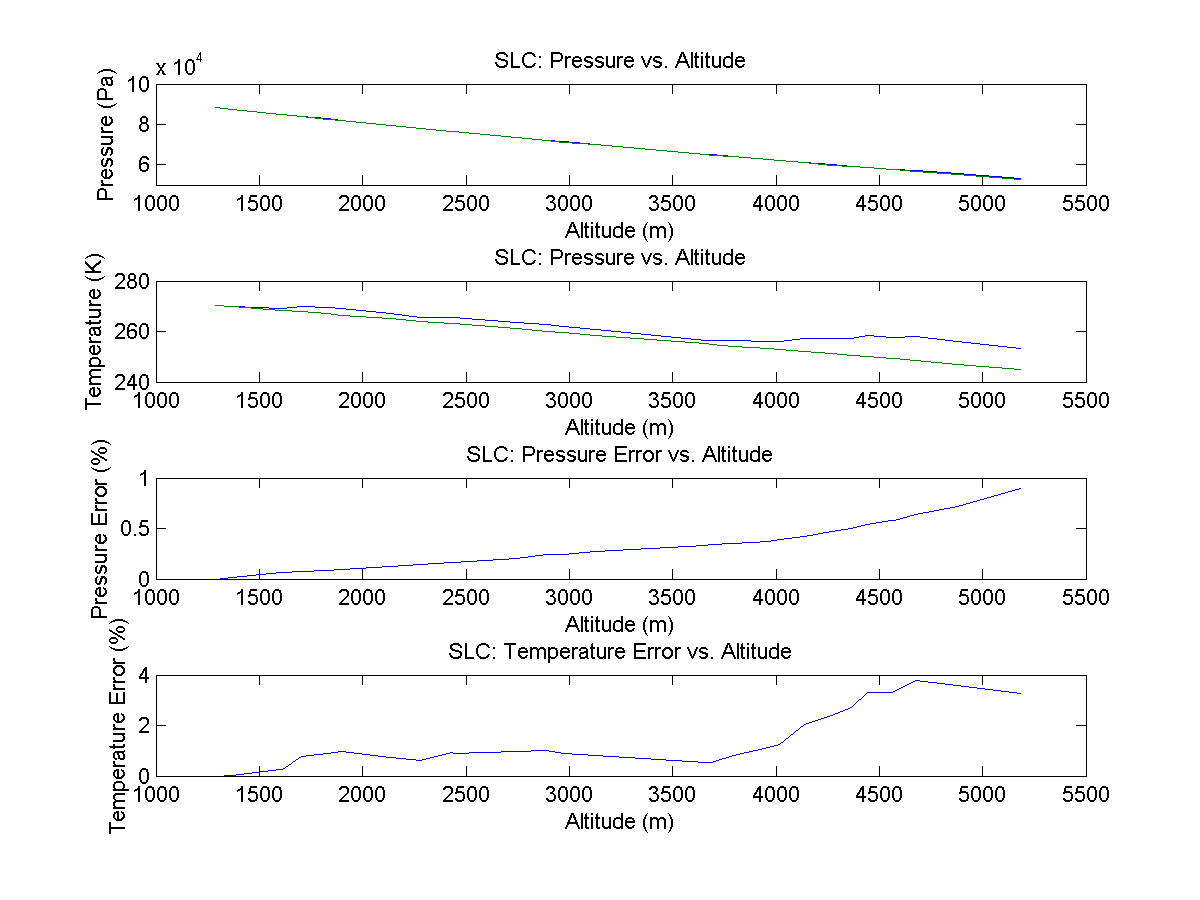
\includegraphics{images/plots/SLC_plot.png}
\caption{Comparison of ISA Model with SLC Weather Balloon Data
\label{atmosphere1_plot_label}}
\end{figure}

\begin{figure}[htbp]
\centering
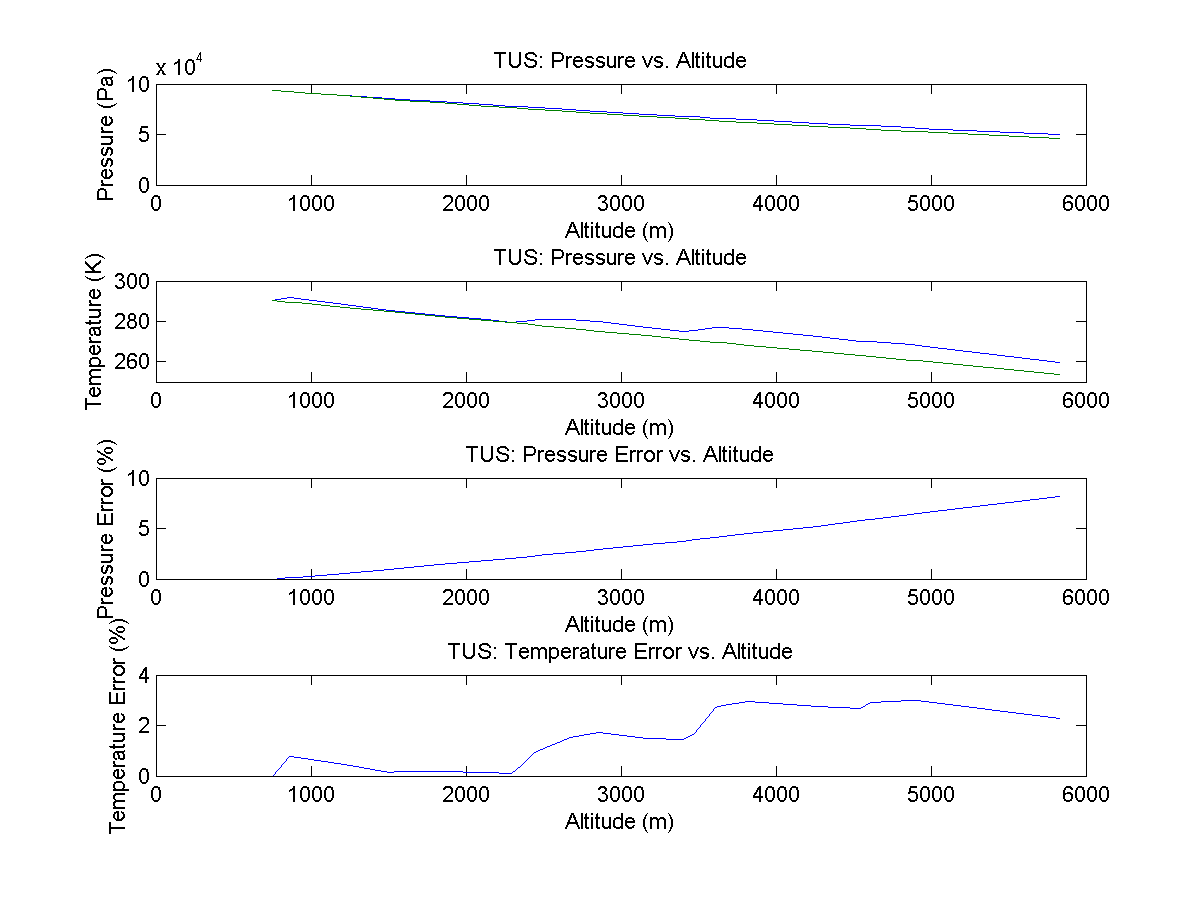
\includegraphics{images/plots/TUS_plot.png}
\caption{Comparison of ISA Model with TUS Weather Balloon Data
\label{atmosphere2_plot_label}}
\end{figure}

The figures show an extremely close alignment with real conditions, both
falling below 1\% error

\section{Flight Validation}\label{flight-validation}

\subsection{University of Louisville}\label{university-of-louisville}

The University of Louisville was kind enough to share experimental
rocket flight data, as well as their rocket dimensions so that our
simulation could be compared to real-world experimental data.

\section{Flight Details}\label{flight-details}

March 29, 2015

\begin{longtable}[c]{@{}llllll@{}}
\toprule
Date & Elevation & Ground Temperature & Wind Speed & Humidity & Launch
Guide Length\tabularnewline
\midrule
\endhead
2015/03/29 & 405 ft (123,48 m) & 289.26 K (61.00 \(^\circ\)F) & 14 km/h
(3.89 m/s) & \textasciitilde{}39 \% & 3.05 m\tabularnewline
2015/03/29 & 432 ft (131.71 m) & 287.71 K (58.21 \(^\circ\)F) & 14 km/h
(3.89 m/s) & \textasciitilde{}39 \% & 3.05 m\tabularnewline
2015/03/29 & 410 ft (125.00 m) & 294.70 K (70.79 \(^\circ\)F) & 14 km/h
(3.89 m/s) & \textasciitilde{}39 \% & 3.05 m\tabularnewline
2015/03/29 & 417 ft (127.13 m) & 289.44 K (61.32 \(^\circ\)F) & 14 km/h
(3.89 m/s) & \textasciitilde{}39 \% & 3.05 m\tabularnewline
2015/03/29 & 446 ft (135.97 m) & 289.54 K (61.50 \(^\circ\)F) & 14 km/h
(3.89 m/s) & \textasciitilde{}39 \% & 3.05 m\tabularnewline
\bottomrule
\end{longtable}

\section{Motor Details}\label{motor-details}

Cesaroni L935

\begin{longtable}[c]{@{}ll@{}}
\toprule
Parameter & Value\tabularnewline
\midrule
\endhead
Manufacturer: & Cesaroni Technology\tabularnewline
Entered: & Oct 6, 2009\tabularnewline
Last Updated: & Jun 26, 2014\tabularnewline
Mfr. Designation: & 3147L935-P\tabularnewline
Common Name: & L935\tabularnewline
Motor Type: & reload\tabularnewline
Diameter: & 54.0mm\tabularnewline
Length: & 64.9cm\tabularnewline
Total Weight: & 2542g\tabularnewline
Prop. Weight: & 1567g\tabularnewline
Cert. Org.: & Canadian Association of Rocketry\tabularnewline
Cert. Date: & Aug 27, 2009\tabularnewline
Average Thrust: & 933.8N\tabularnewline
Maximum Thrust: & 1585.6N\tabularnewline
Total impulse: & 3146.8Ns\tabularnewline
Burn Time: & 3.4s\tabularnewline
Isp: & 205s\tabularnewline
Case Info: & Pro54-6GXL\tabularnewline
Propellant Info: & Imax\tabularnewline
Data Sheet: & link\tabularnewline
Availability: & regularCesaroni L935\tabularnewline
\bottomrule
\end{longtable}

\clearpage

\section{Plots}\label{plots}

\begin{figure}[htbp]
\centering
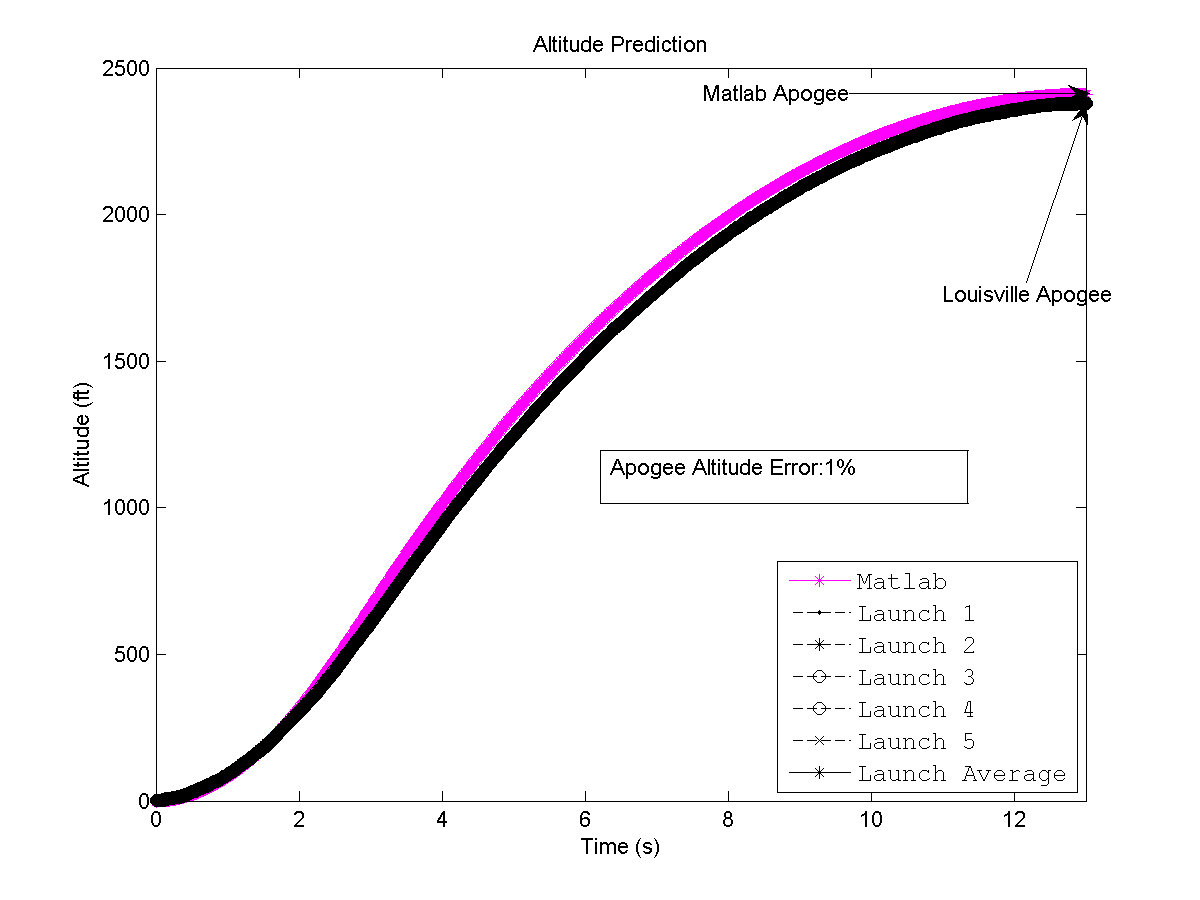
\includegraphics{images/plots/plot_louisville_altitude_analysis.png}
\caption{Altitude Plot of Simulation Data vs Louisville Rocket Launches
\label{experimental_comparison_altitude_label}}
\end{figure}

\begin{figure}[htbp]
\centering
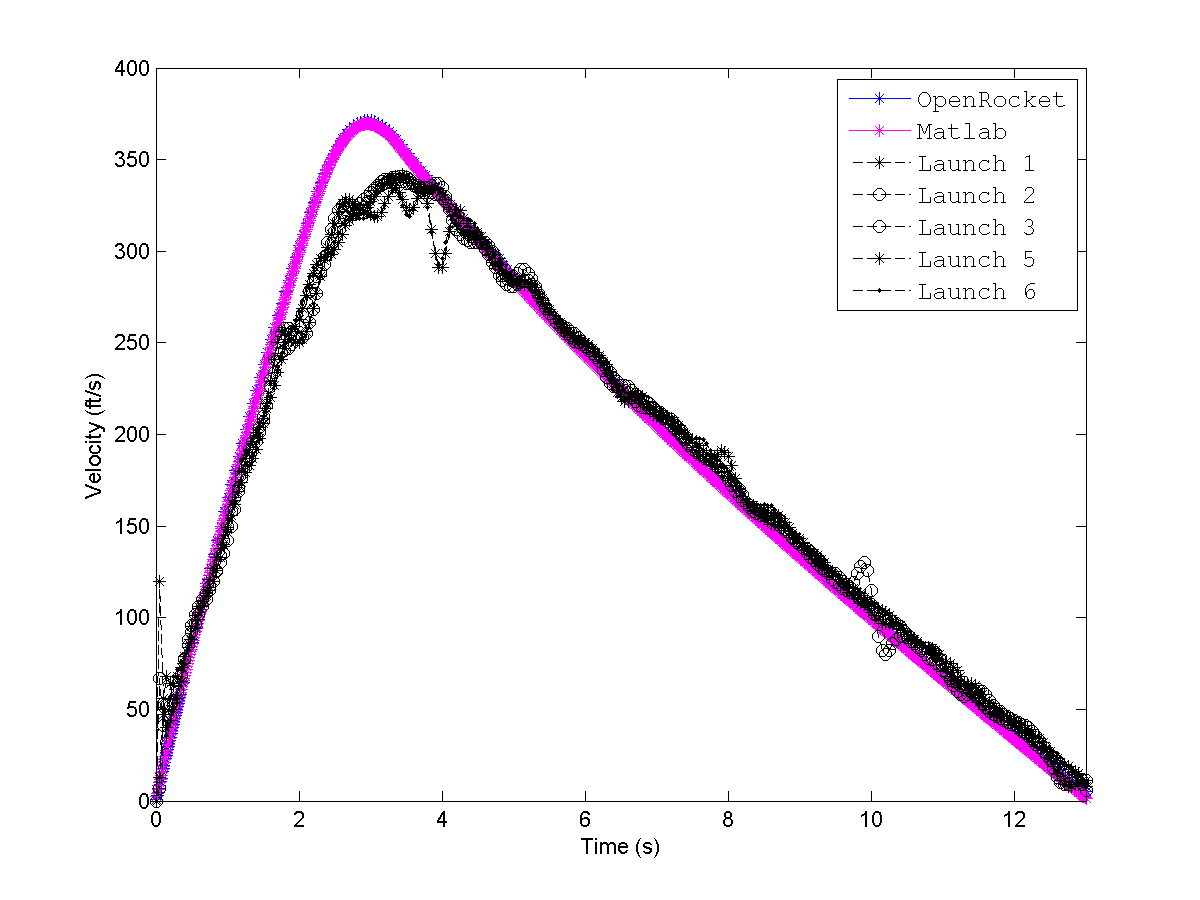
\includegraphics{images/plots/plot_louisville_velocity_analysis.png}
\caption{Velocity Plot of Simulation Data vs Louisville Rocket Launches
\label{experimental_comparison_velocity_label}}
\end{figure}

\clearpage 

\subsection{Comparison with Arcturus
Rocket}\label{comparison-with-arcturus-rocket}

The rocket flown at last years competition was also modeled. As shown in
Figures \ref{arc_experimental_comparison_altitude_label} and
\ref{arc_experimental_comparison_velocity_label}, a high degree of
accuracy with the avionics data is further confirmed.

\begin{figure}[htbp]
\centering
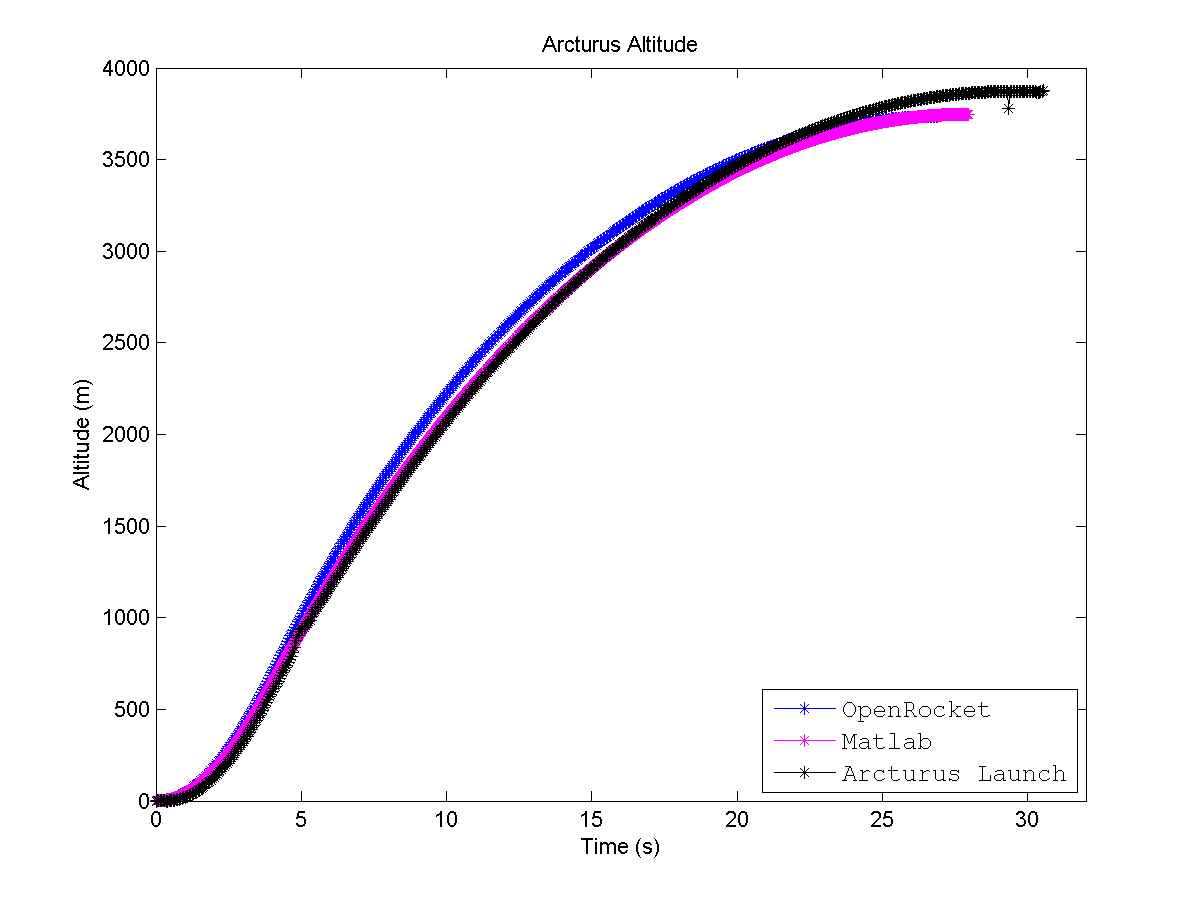
\includegraphics{images/plots/plot_arcturus_altitude_analysis.png}
\caption{Altitude Plot of Simulation Data vs Arcturus Rocket Launch
\label{arc_experimental_comparison_altitude_label}}
\end{figure}

\begin{figure}[htbp]
\centering
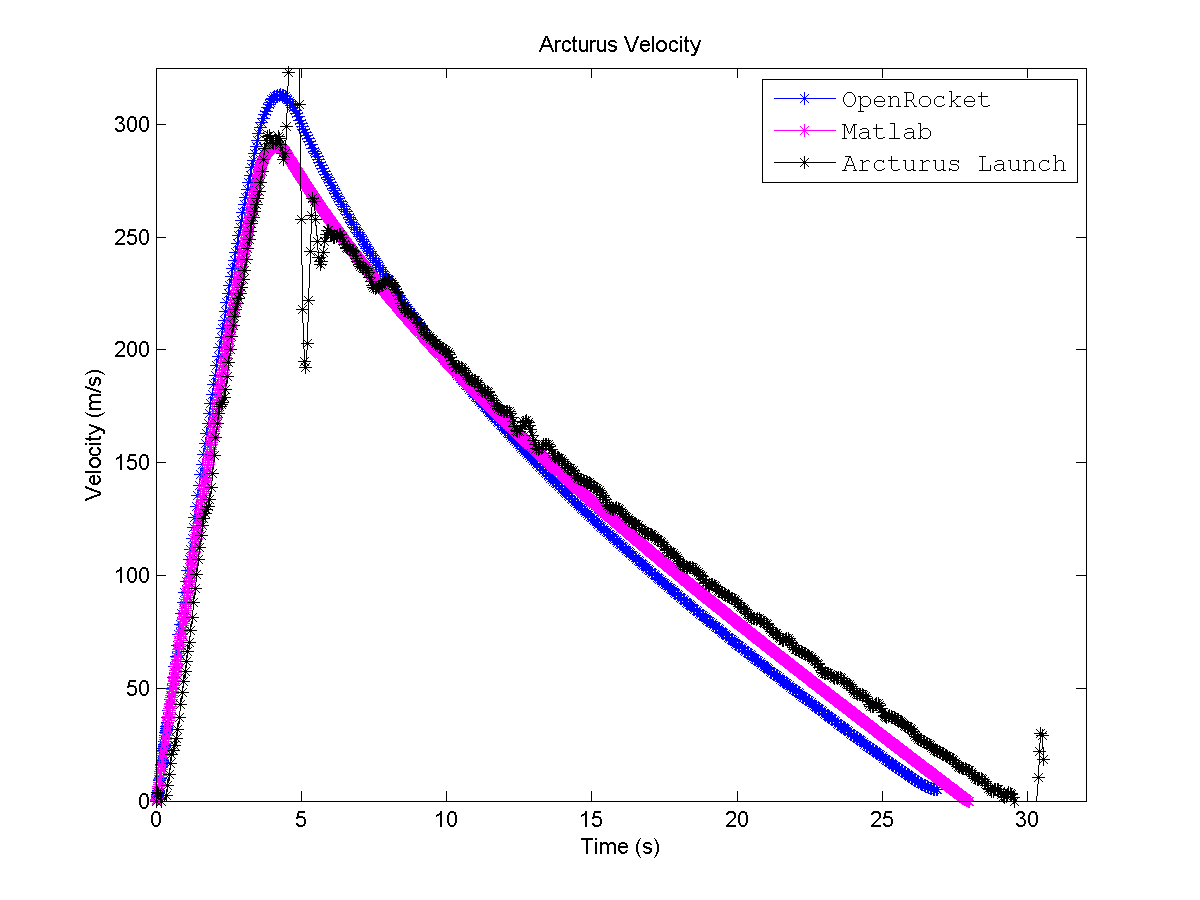
\includegraphics{images/plots/plot_arcturus_velocity_analysis.png}
\caption{Velocity Plot of Simulation Data vs Arcturus Rocket Launch
\label{arc_experimental_comparison_velocity_label}}
\end{figure}

\section{Summary of Comparison with Experimental
Data}\label{summary-of-comparison-with-experimental-data}

\begin{longtable}[c]{@{}lll@{}}
\toprule
Data Source & Parameter Tested & \% Error\tabularnewline
\midrule
\endhead
Weather Balloon Data (Salt Lake City, UT) & Pressure with Altitude &
\textless{} 1\%\tabularnewline
Weather Balloon Data (Tuscon, AZ) & Pressure with Altitude & \textless{}
1\%\tabularnewline
University Of Louisville (avg. of 5 Launches) & Altitude &
1\%\tabularnewline
University Of Louisville (avg. of 5 Launches) & Velocity &
9\%\tabularnewline
Arcturus Flight Launch & Altitude & 3\%\tabularnewline
Arcturus Flight Launch & Velocity & 1\%\tabularnewline
\bottomrule
\end{longtable}

\captionof{table}{Summary of Comparison with Experimental Data}

\chapter{Simulation Execution}\label{simulation-execution}

\section{Simulation Configuration}\label{simulation-configuration}

\subsection{Historical Weather Data for Green River,
Utah}\label{historical-weather-data-for-green-river-utah}

The following conditions are historical data for Green River, Utah on
June 25th, 2015 at 12:00PM (noon) {[}13{]}.

\begin{longtable}[c]{@{}llllll@{}}
\toprule
Date & Elevation & Ground Pressure & Ground Temperature & Wind Speed &
Humidity\tabularnewline
\midrule
\endhead
2015/06/15 & 4,078 ft (1,243 m) & 101300 Pa & 298.15 K (25 \(^\circ\)C)
& 6 km/h (1.6 m/s) & 33 \%\tabularnewline
2014/06/15 & 4,078 ft (1,243 m) & 100700 Pa & 296.15 K (23 \(^\circ\)C)
& 20 km/h (5.56 m/s) & 8 \%\tabularnewline
2013/06/15 & 4,078 ft (1,243 m) & 101000 Pa & 299.15 K (26 \(^\circ\)C)
& 10 km/h (2.78 m/s) & 19 \%\tabularnewline
\bottomrule
\end{longtable}

\captionof{table}{Historical Weather Conditions, Green River, Utah}

\subsection{General Conditions}\label{general-conditions}

\begin{longtable}[c]{@{}lll@{}}
\toprule
Elevation & Humidity & Launch Guide Length\tabularnewline
\midrule
\endhead
4300 ft (1,311 m) & 33 \% & 5.4864 (18 ft)\tabularnewline
\bottomrule
\end{longtable}

\captionof{table}{General Simulation Conditions}

\subsection{Best Case}\label{best-case}

The best case scenario is with no wind, and a 0\(^\circ\) launch angle,
and the lowest air pressure.

\begin{longtable}[c]{@{}llll@{}}
\toprule
Wind Speed & Ground Pressure & Ground Temperature & Launch Guide
Angle\tabularnewline
\midrule
\endhead
0 m/s & 101000 Pa & 298.15 K (25 \(^\circ\)C) &
0\(^\circ\)\tabularnewline
\bottomrule
\end{longtable}

\captionof{table}{Best Case Simulation Conditions}

\subsection{Worst Case}\label{worst-case}

The worst case scenario, is the maximum wind condition permitted for
launch by the competition, and a launch guide angle, and the highest
pressure.

\begin{longtable}[c]{@{}llll@{}}
\toprule
Wind Speed & Ground Pressure & Ground Temperature & Launch Guide
Angle\tabularnewline
\midrule
\endhead
8.33 m/s & 101325 kPa & 303.15 K (30 \(^\circ\)C) &
10\(^\circ\)\tabularnewline
\bottomrule
\end{longtable}

\captionof{table}{Worst Case Simulation Conditions}

\clearpage

\section{Simulation Execution}\label{simulation-execution-1}

Identical rocket designs were implemented in OpenRocket, RockSim,
RASAero, and our Engineering Simulator. The 3rd party simulator results
were parsed with Matlab to determine essential performance criteria and
to compare with our model.

\clearpage

\subsection{Matlab}\label{matlab}

\subsubsection{Matlab Models}\label{matlab-models}

\begin{figure}[htbp]
\centering
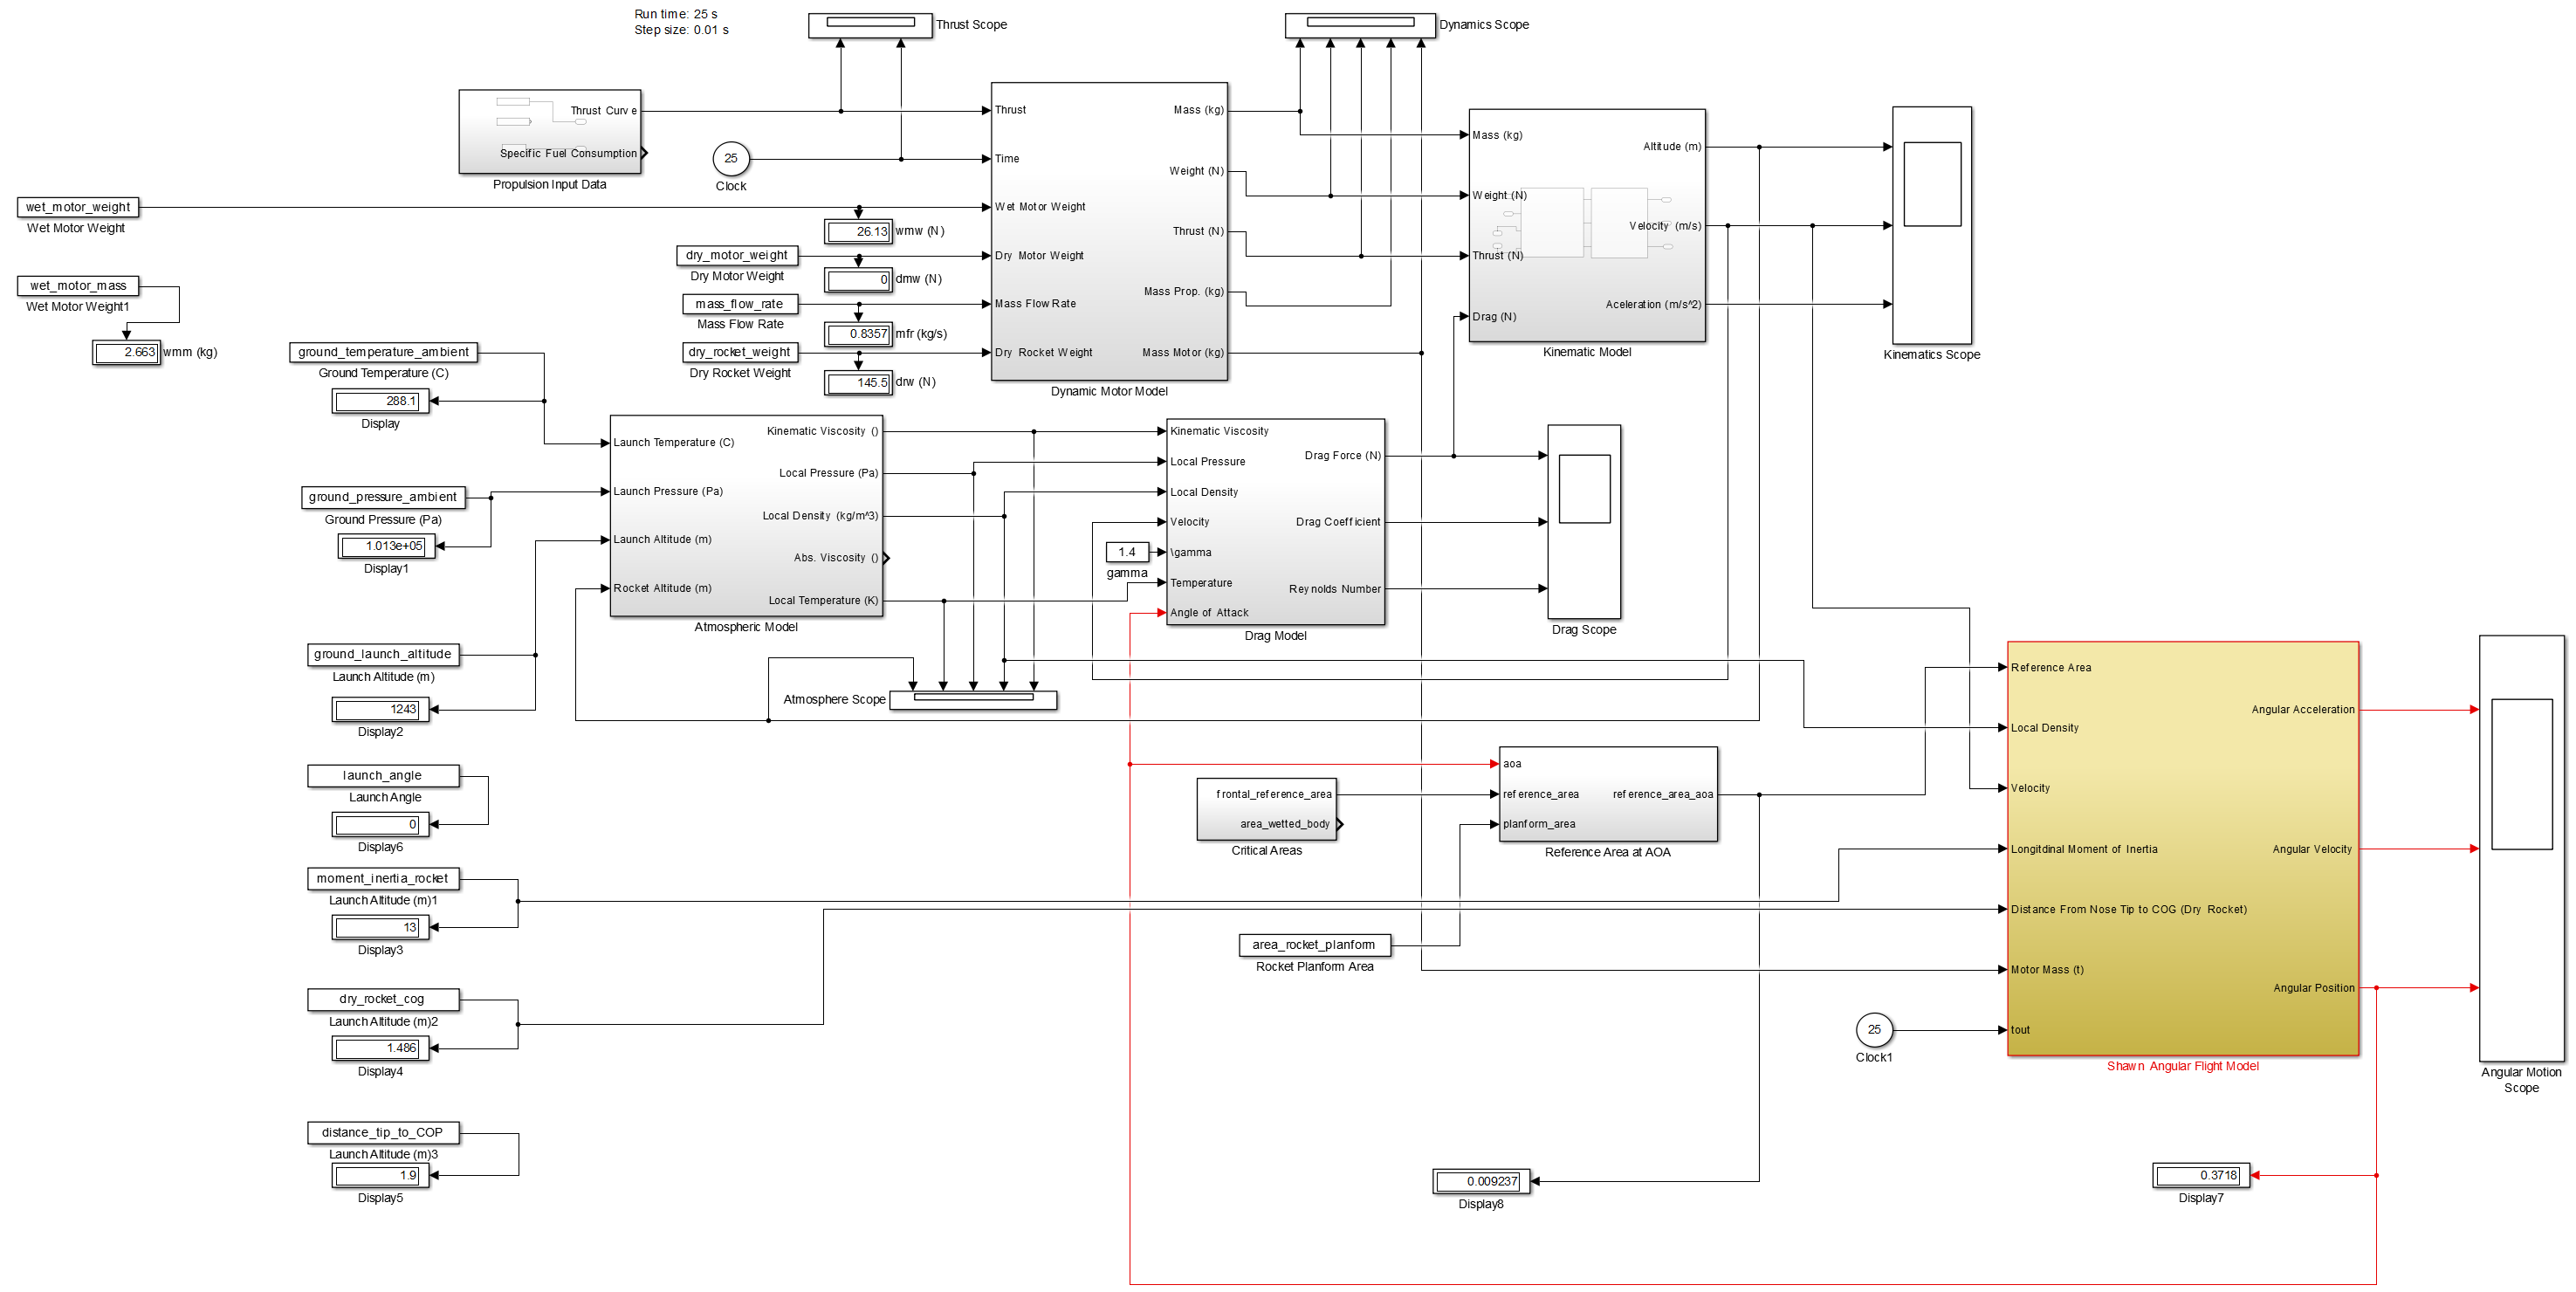
\includegraphics{images/rocket_model.png}
\caption{Full Model in Simulink, angle-of- attack less than 15 degrees
\label{full_model_test_label}}
\end{figure}

\clearpage

\section{Observations}\label{observations}

Figure \ref{error_altitude_plot_label} shows the predicted Altitude of
the rocket compared against OpenRocket, RASAero, and Rocksim. It would
appear that RASAero and Rocksim predict a higher altitude, perhaps
considering their underestimation of the drag forces, shown in Figure
\ref{error_dragforce_v_plot_label}.

\begin{figure}[htbp]
\centering
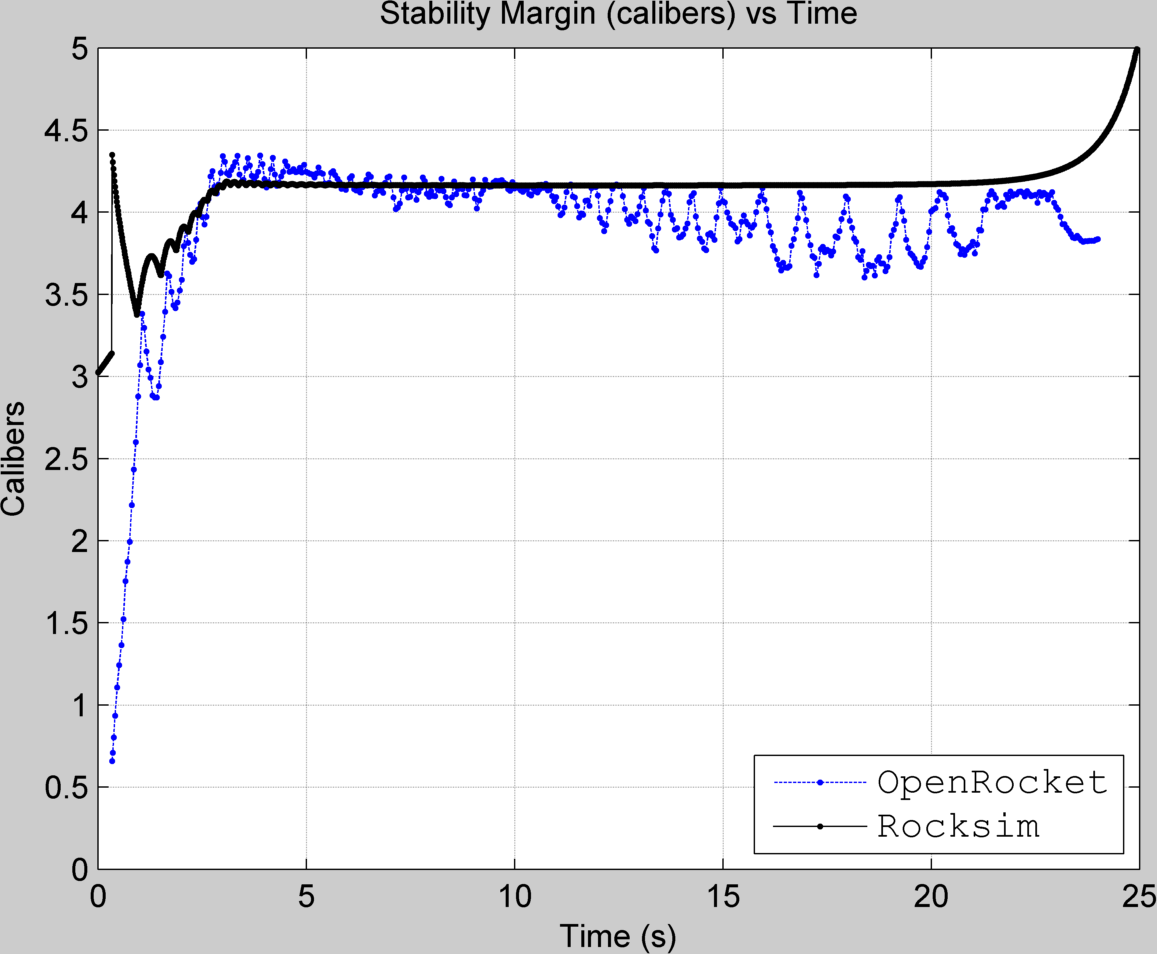
\includegraphics{images/plots/error_altitude_plot.png}
\caption{Altitude as a Function of Time
\label{error_altitude_plot_label}}
\end{figure}

\begin{quote}
2e Vehicle reaches 10,000 ft altitude (+1000 feet / - 0 feet)
\end{quote}

\clearpage

Figure \ref{error_mach_plot_label} shows that the Mach number predicted
by each software is quite close.

\begin{figure}[htbp]
\centering
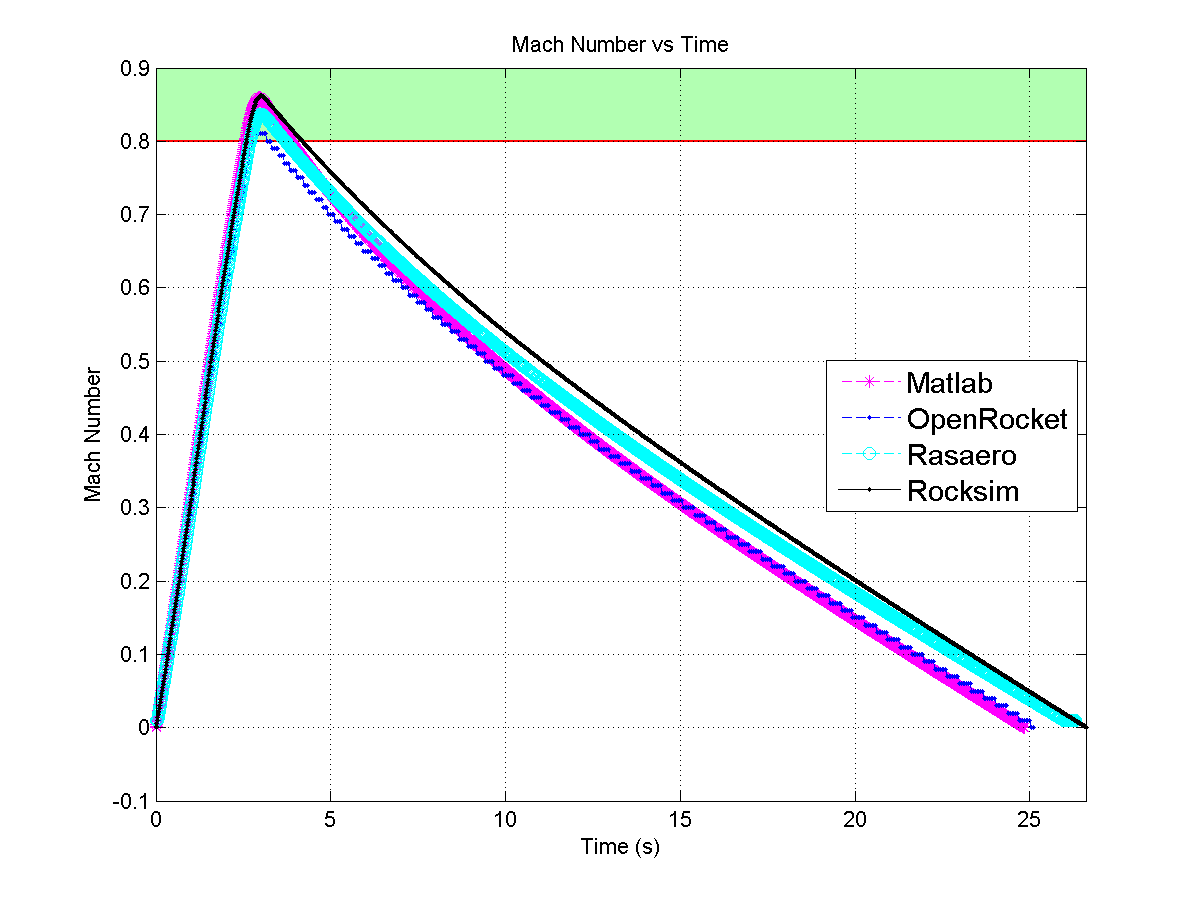
\includegraphics{images/plots/error_mach_plot.png}
\caption{Mach Number as a Function of Time
\label{error_mach_plot_label}}
\end{figure}

\begin{quote}
2d Vehicle max speed mach 0.9
\end{quote}

\clearpage

Figure \ref{error_stability_calibers_plot_label} shows that the dynamic
stability is quite similarly predicted by all tested simulators.
OpenRocket shows a continuous oscillation, which according to my current
analysis of their methodology, perhaps does not correctly consider the
oscillation damping encountered during flight. In any case, if the
OpenRocket model were to be 100\% correct, the dynamic stability
criteria would still be satisfied by a wide margin.

\begin{quote}
2a Static stability above 2 calibers
\end{quote}

\begin{quote}
2b Dynamic stability above 0
\end{quote}

\begin{figure}[htbp]
\centering
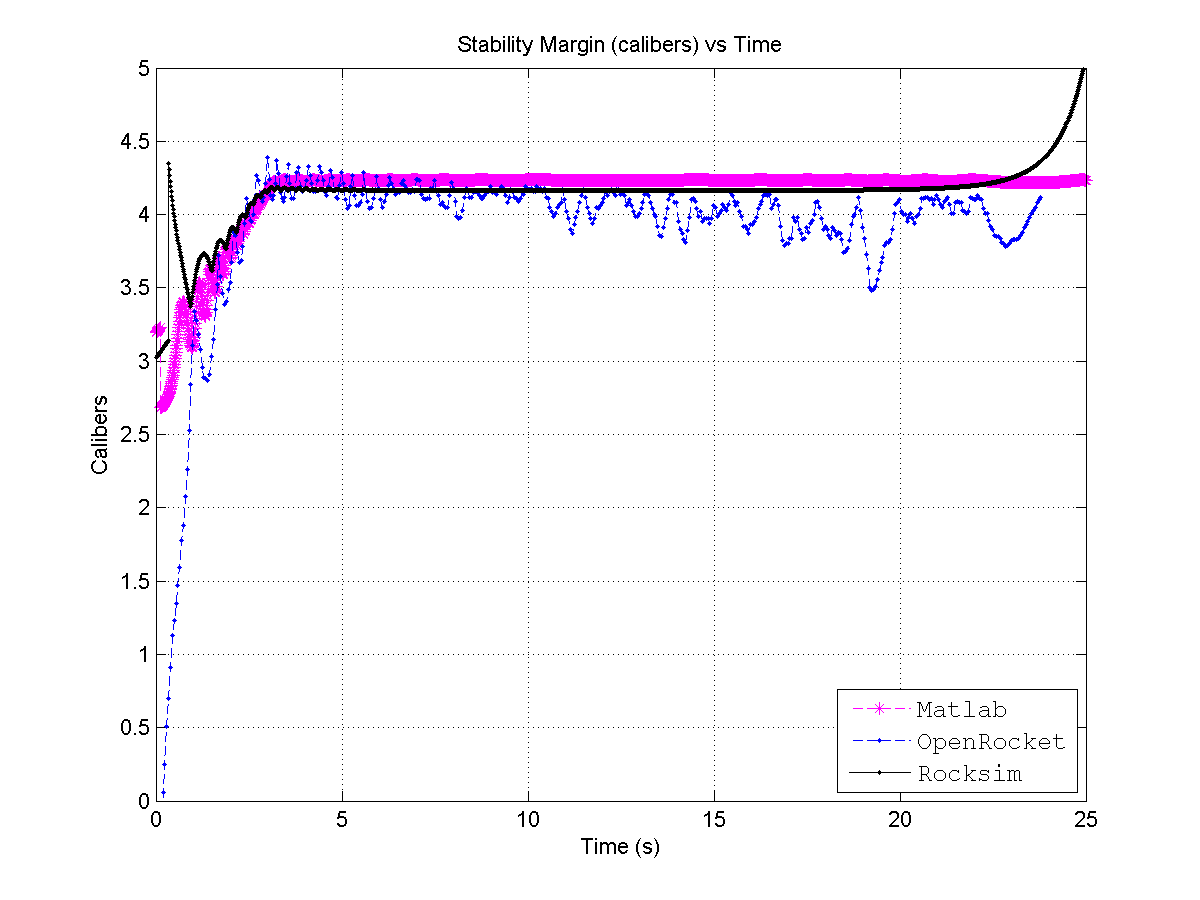
\includegraphics{images/plots/error_stability_calibers_plot.png}
\caption{Stability (Calibers) as a Function of Time
\label{error_stability_calibers_plot_label}}
\end{figure}

\clearpage
As seen in Figure \ref{plot_natural_frequency}, once the rocket leaves
the launch pad, the angular frequency of the rigid-body oscillation does
not approach the natural frequency of the rocket, confirming
requirement:

\begin{quote}
2f - The vehicle does not experience resonant pitching/yawing motion in
flight
\end{quote}

In any case, we know that resonant oscillation at the natural frequency
does not occur, since the rocket stabilizes. Figure
\ref{error_stability_response} shows the stabilization of the
angle-of-attack with time.

\begin{figure}[htbp]
\centering
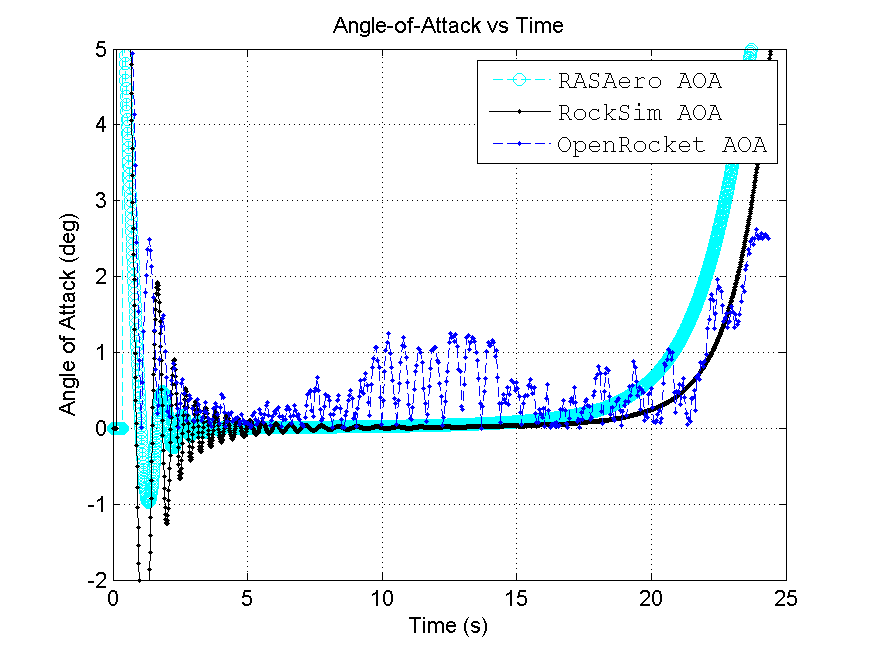
\includegraphics{images/plots/error_aoa_plot.png}
\caption{Angle of Attack Stabilization \label{error_stability_response}}
\end{figure}

RockSim and RASAero are chosen for this plot since they have a more
mature stability methodology.

\begin{figure}[htbp]
\centering
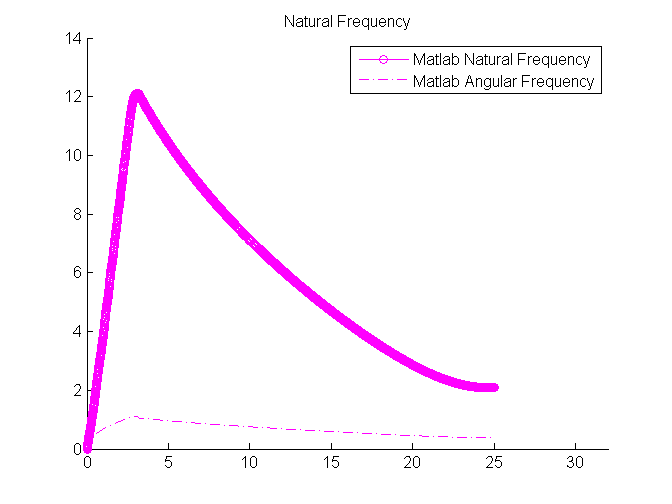
\includegraphics{images/plots/plot_natural_frequency.png}
\caption{Natural Frequency \label{plot_natural_frequency}}
\end{figure}

\clearpage

\section{Simulation Summary}\label{simulation-summary}

\begin{figure}[htbp]
\centering
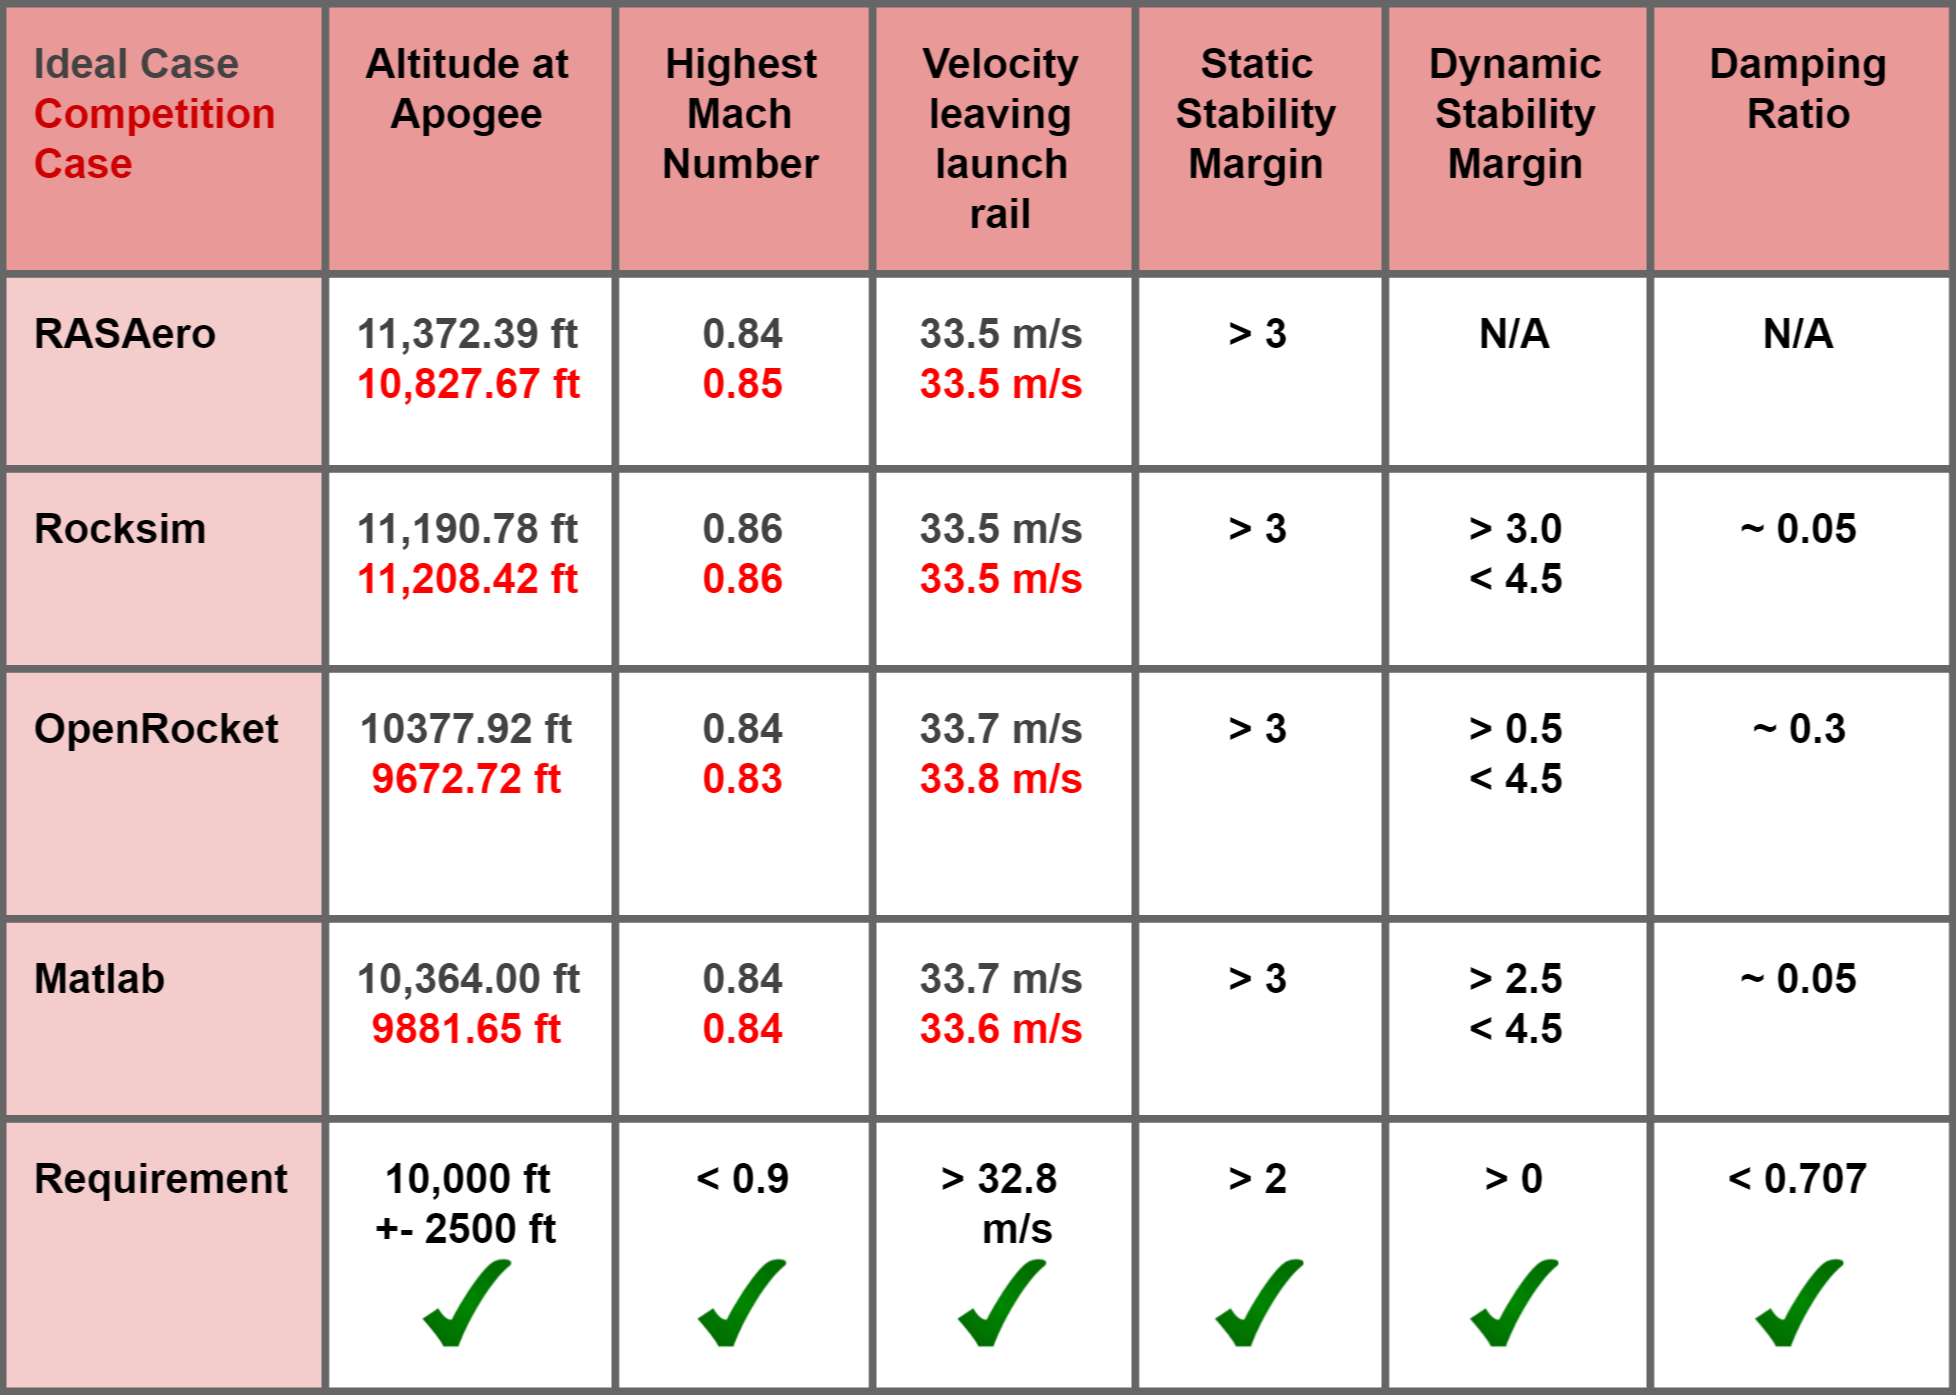
\includegraphics{images/simulation_summary.png}
\caption{Simulation Summary \label{plt_simulation_summary}}
\end{figure}

\clearpage

\chapter{Future Enhancements}\label{future-enhancements}

\section{Hardware-in-the-loop}\label{hardware-in-the-loop}

\section{Porting to Python /
OpenModelica}\label{porting-to-python-openmodelica}

\section{Plotting with Plot.ly}\label{plotting-with-plot.ly}

\section{Robust Wind Model}\label{robust-wind-model}

To account for wind turbulence in future models, two commonly used Wind
Models are explored.

\subsubsection{Kaimal Wind Model}\label{kaimal-wind-model}

\begin{equation}
\label{eq_kaiman_wind_model}
\dfrac{S_u (f)}{\sigma ^2 _ u} = \dfrac{4 L_{1u} / U }{(1+6f L_{1u} / U )^{5/3}}
\end{equation}

\subsubsection{Von Karman Wind Model}\label{von-karman-wind-model}

\begin{equation}
\label{eq_von_karman_wind_model}
\dfrac{S_u (f)}{\sigma ^2 _ u} = \dfrac{4 L_{2u} / U }{(1+ 70.8 (fL_{2u} / U)^2 )^{5/3}}
\end{equation}

Where

\begin{itemize}
\tightlist
\item
  \(\dfrac{S_u (f)}{\sigma ^2 _ u}\) is the \emph{Spectral Density
  Function} of turbulence velocity
\item
  \(f\) is the turbulence frequency
\item
  \(\sigma_u\) is the standard deviation fo the turbulence velocity
\item
  \(L_{1u}\) and \(L_{2u}\) are length parameters
\item
  \emph{U} is the average wind speed
\end{itemize}

{[}4{]}

\section{ThrustCurve.org API
Integration}\label{thrustcurve.org-api-integration}

ThrustCurve.org has an API we could use to dynamically pull motor data
for integration into the simulation

\section{Rocket Orientation}\label{rocket-orientation}

While good results have been achieved thus far, a 6DOF simulator is
preferable to produce the most realistic simulation possible. It would
be possible to account for wind turbulence and other disruptions which
are not confined to a single axis. If all forces and moments can be
clearly defined, it also allows a seamless coupling of the point-mass
and rigid body rotation systems described earlier, as well as the
pitch/yaw and roll systems.

Building on the material explored in the Angular Stability model, this
section introduces topics relating to the orientation of the rocket
during flight.

\begin{figure}[htbp]
\centering
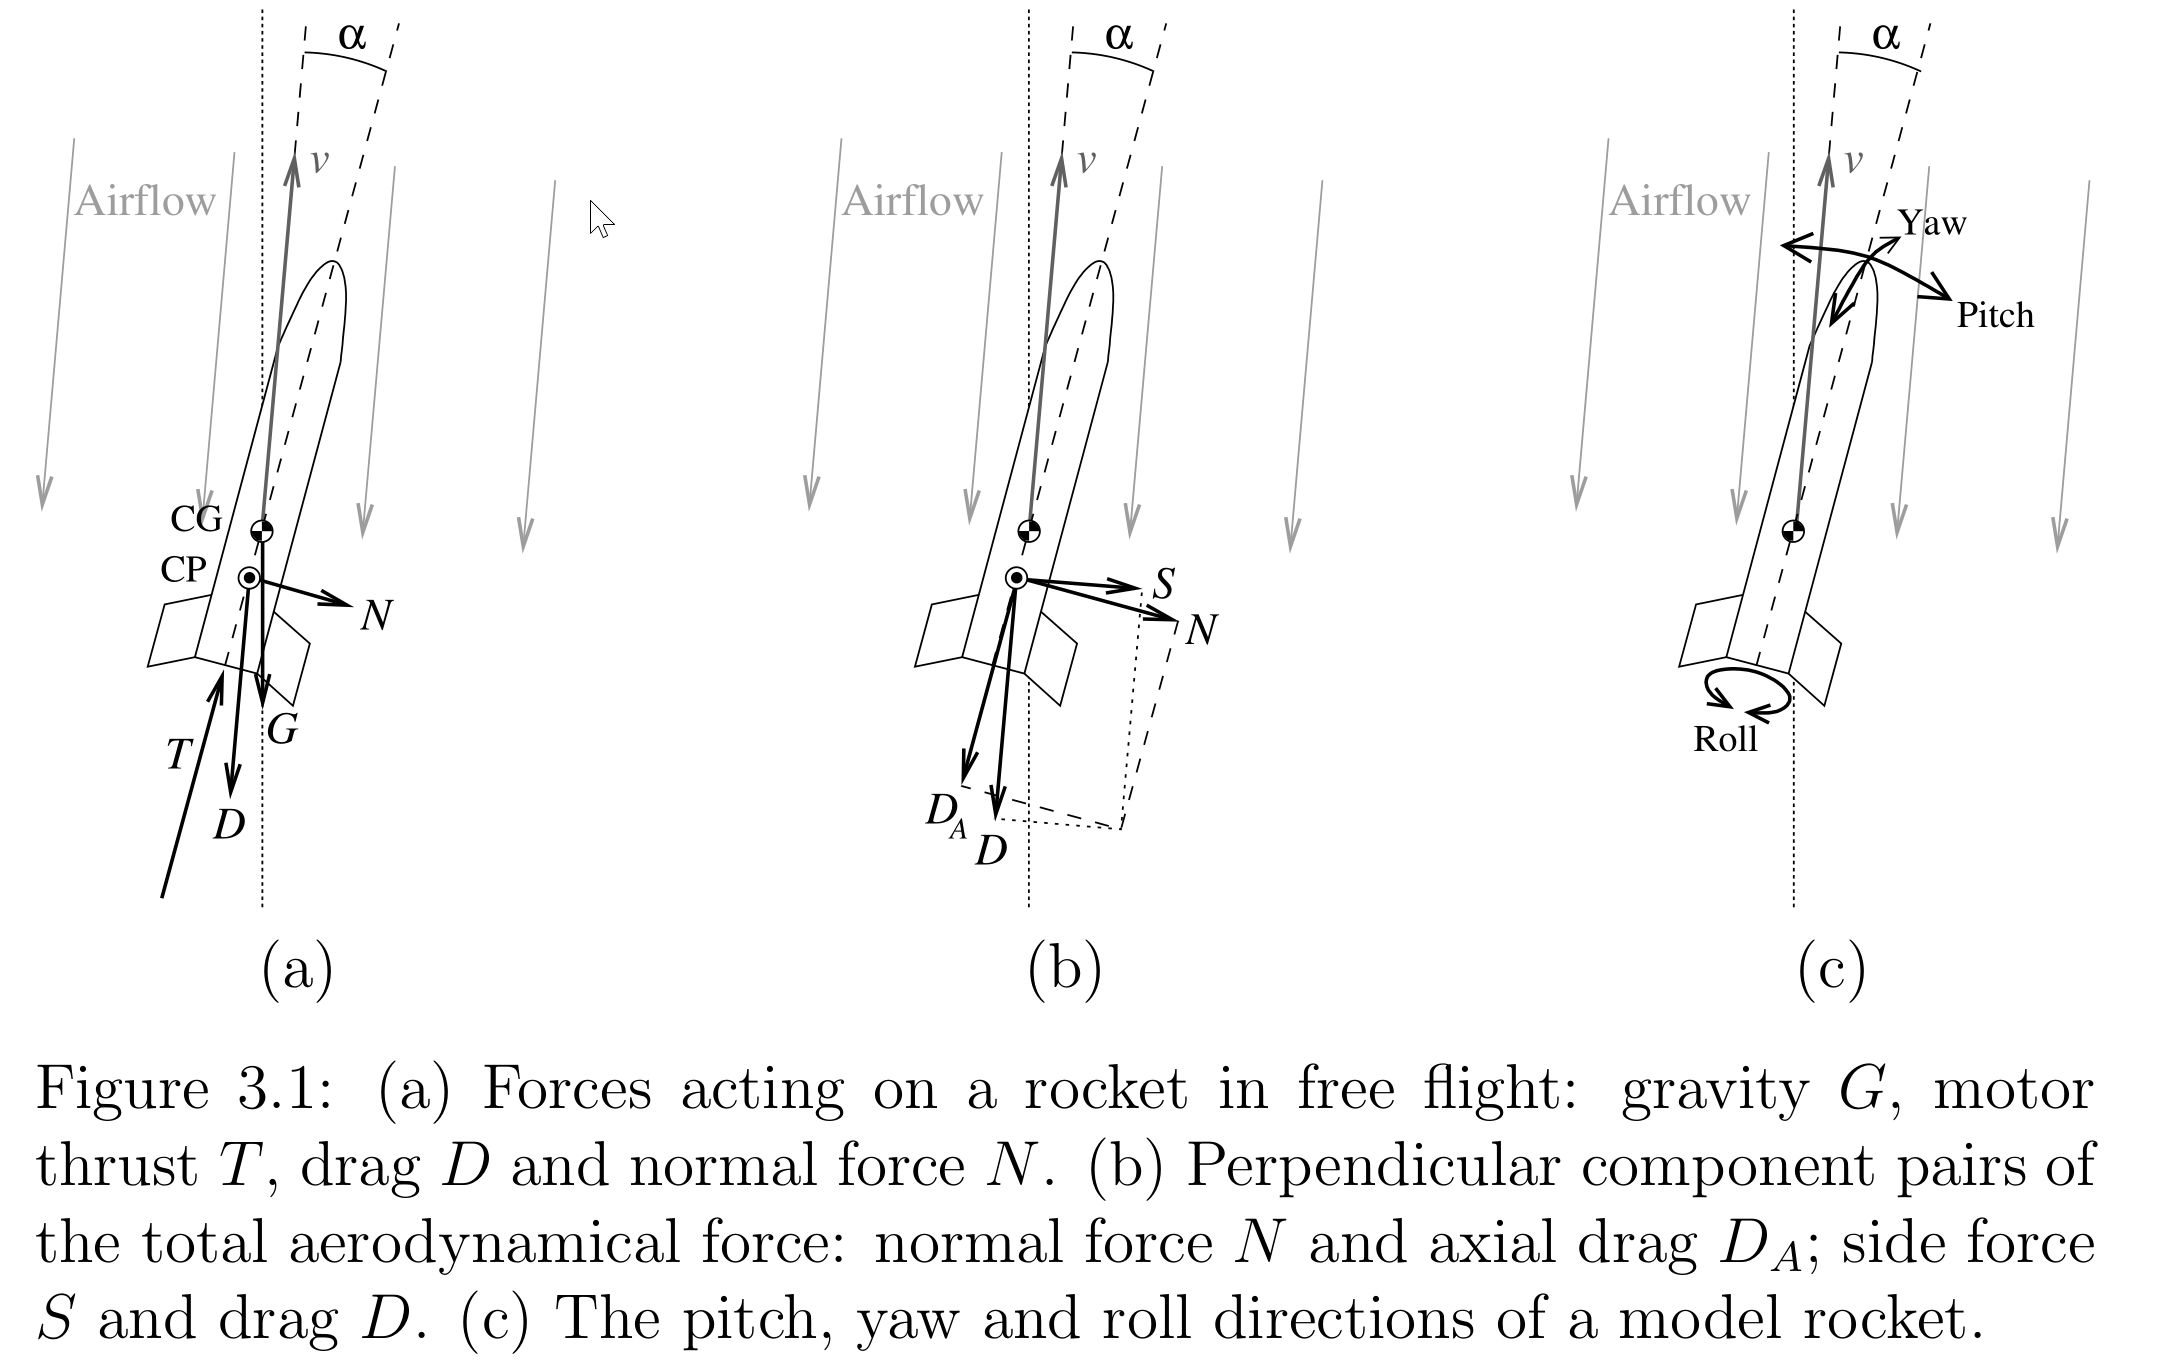
\includegraphics{images/rocket_flight_forces_moments.png}
\caption{Forces and Moments Experienced by rocket in flight
\label{img_rocket_flight_forces_moments_label}}
\end{figure}

\clearpage

\subsection{Rotations}\label{rotations}

\emph{Spherical Coordinates} and \emph{Euler Angles} are commonly used
to describe the orientation of an object, however both systems encounter
singularities where the orientation is ambiguous. Special cases are
required to handle these singularities, which complicate the analysis
and programming.

\subsection{Quaternions}\label{quaternions}

\emph{Quaternions} are commonly used to describe spatial rotation,
avoiding singularities.

An initial position is taken as reference to describe subsequent changes
in orientation. Vectors can be transformed from rocket coordinates to
world coordinates, and the reverse.

Leonhard Euler proved that

\begin{equation}
\label{eq_euler_mult}
e^{i\phi} = \cos \phi + i \sin \phi
\end{equation}

Thus, \(e^{i\phi}\) lies on the unit circle in the complex plane, and
has a unit length.

Multiplication

\[
(a+bi)(c+di) = re^{i\phi}se^{i\phi} = rse^{i(\phi + \theta)}
\]

\[
i^2 = j^2 = k^2 = ijk = -1
\]

Quaternions

\[
H = { a + bi + cj + dk : a,b,c,d \forall R }j
\]

\(i\), \(j\), \(k\) are all square roots of \(-1\)

\[
ij = k = -ji 
\] \[
jk = i = -kj 
\] \[
ki = j = -ik
\]

If we consider three-dimensional space to be purely imaginary
quaternions:

\[
R^3 = {xi + yj + zk : x,y,z \forall R}
\]

Rotations are done using unit quaternions

\[
\cos \phi + i \sin \phi 
\] \[
\cos \phi + j \sin \phi 
\] \[
\cos \phi + k \sin \phi
\] Which can be rewritten as

\[
e^{i\phi}, e^{i\phi}, e^{k\phi}
\]

For example, taking any arbitrary unit quaternion (\emph{vector})
\textbf{u}

\[
u = u_1i + u_2j + u_3k = e^{u\phi}
\]

We can rotate another arbitrary vector \textbf{v} about the axis in the
\textbf{u} direction

\[
e^{u\phi}ve^{-u\phi}
\]

http://math.ucr.edu/\textasciitilde{}huerta/introquaternions.pdf

\subsection{Parameters needed for quaternion
analysis}\label{parameters-needed-for-quaternion-analysis}

\begin{itemize}
\tightlist
\item
  rocket mass
\item
  \textbf{reference length}
\item
  angle-of-attack
\item
  reference area
\item
  longitudinal moment of inertia
\item
  radial moment of inertia
\item
  thrust force
\item
  drag force
\item
  weight force
\item
  pitching moment
\item
  pitch damping moment
\item
  yawing moment
\item
  yaw damping moment
\item
  \sout{roll moment}
\item
  \sout{roll forcing moment}
\item
  \sout{roll damping moment}
\item
  normal force
\item
  side force
\item
  pitch rate
\item
  raw rate
\item
  roll rate
\item
  wind velocity
\end{itemize}

\subsection{Rocket Moments}\label{rocket-moments}

A \emph{Pitch Moment} and \emph{Pitch Damping Moment} are defined, which
are different than the \emph{Corrective Moment Coefficient} and the
\emph{Damping Moment Coefficient}. Note: a complementary \emph{Yaw
Moment} and \emph{Yaw Damping Moment} are implied, with exactly the same
considerations for motion along the uncoupled complementary yaw-axis.

\subsection{Pitch Moment}\label{pitch-moment}

The \emph{Pitch Moment} is taken from the tip of the nose cone, it must
be moved to the COG to mirror \emph{Corrective Moment Coefficient}.

\begin{equation}
\label{eq_pitching_moment}
M_{pm}(x) = - \dfrac{1}{2} \rho v^2 C_m A_{ref} * L_{ref}
\end{equation}

TODO why minus?

Where:

\begin{itemize}
\tightlist
\item
  \(\rho\) is the local atmospheric density
\item
  \(v\) is the rocket velocity relative to the surrounding air
\item
  \(A_ref\) is the reference area (frontal or side?)
\item
  \(L_{ref}\) is ???
\end{itemize}

\subsection{Pitch Moment Coefficient}\label{pitch-moment-coefficient}

\begin{equation}
\label{eq_pitch_moment}
C_m = C_m - F_s \cdot COG \cdot L_{ref} 
\end{equation}

Where:

\begin{itemize}
\tightlist
\item
  \(F_s\) is the side force
\end{itemize}

\subsection{Fin-set Pitch Moment
Coefficient}\label{fin-set-pitch-moment-coefficient}

\begin{equation}
M_{pm} = \dfrac{C_N \times COP}{L_{ref}}
\end{equation}

\subsection{Body Tube and Fin Set Interference Pitch Moment
Coefficient}\label{body-tube-and-fin-set-interference-pitch-moment-coefficient}

\begin{equation}
M_{pm} = \dfrac{C_N \times COP_x}{L_{ref}}
\end{equation}

\subsection{Barrowman Calculation}\label{barrowman-calculation}

\begin{equation}
total.getCM + forces.getCM
\end{equation}

\subsection{Final Solver Pitch Moment
Coefficient}\label{final-solver-pitch-moment-coefficient}

\begin{equation}
M_{pm} = M_{pm} + \left( \text{randomness}  \right)
\end{equation}

Some randomness is added to avoid an ``over-perfect'' solution

\subsection{Pitch Damping Moment}\label{pitch-damping-moment-1}

\begin{itemize}
\tightlist
\item
  significant only near apogee
\end{itemize}

\section{Stochastic Simulations}\label{stochastic-simulations}

The simulator described in this paper is deterministic. It assumes that
all input parameters are known and produces the same simulation result
each time it is run, as long as no parameters are directly changed.
While it was acknowledged that conditions may vary and produce different
launch outcomes, only the extreme expected cases were tested - a
multitude of possibilities exist in between.

A convincing and complete engineering simulation must account for the
uncertainties of certain variables. In high-powered rocket flight, there
are many such uncertainties. For example, any error in the shaping of
the fins introduces roll during flight, which has many influences on the
rocket. Additionally, wind turbulence is extremely difficult to predict,
and can have impacts all all stages of the rocket flight which may
change its directory. Temperature is a significant factor for the
performance of the motor - for instance, its total impulse and burn time
are sure to be affected at high temperatures.

The variation of all these parameters together creates a great deal of
uncertainty, which must be accounted for in a robust engineering
simulation.

Stochastic methods such as the \emph{Monte Carlo} method randomize these
parameters and provides a range of uncertainty from which it is possible
to consider the probability that a given simulation outcome will occur
in reality.

\chapter{Conventions}\label{conventions}

\section{Data Model}\label{data-model}

The \emph{Data Model} provides static and dynamics parameters as needed
by other models in the simulation.

\subsection{Static Parameters}\label{static-parameters-1}

Many parameters are constant throughout the simulation, notably the
structural dimensions. All structural dimensions are generated in the
CATIA Design and output to a spreadsheet, which the simulation will load
and place in the Matlab workspace.

This instance can be accessed by multiple models to clearly and
effectively provide parameter access.

\subsection{Dynamic Parameters}\label{dynamic-parameters-1}

As discussed in the \emph{Dynamic Parameters} section, many parameters
are changing due to flight conditions. An additional \emph{Map
Container} instance is created to handle and deliver these changes to
the models that need them.

\section{Matlab Conventions}\label{matlab-conventions}

\section{Matlab/Simulink Libraries}\label{matlabsimulink-libraries}

\section{Overview}\label{overview-3}

The goal is to create a robust Simulink model that references Matlab
code from files that can be tracked by versioning software (Git). The
Matlab source should be editable and effect changes in the Simulink
model.

By a combination of both, full versioning control can be achieved in the
project.

\section{Creating a Library}\label{creating-a-library}

\begin{enumerate}
\def\labelenumi{\arabic{enumi}.}
\tightlist
\item
  Open Matlab
\item
  Open Simulink
\item
  Click File --\textgreater{} New --\textgreater{} Library
\end{enumerate}

\section{Add to path}\label{add-to-path}

Permanently add your workspace to the Matlab path. At the command
prompt:

\begin{verbatim}
>> pathtool
\end{verbatim}

\href{http://www3.nd.edu/~nancy/Math20550/Homework/matlabpath.pdf}{Alternatively,
try this howto}

\section{Add to Library Browser}\label{add-to-library-browser}

\href{http://www.mathworks.com/help/simulink/ug/adding-libraries-to-the-library-browser.html}{Add
to Library Browser}

\section{Algebraic Loops}\label{algebraic-loops}

With systems that involve direct-feedthrough (feedback), it is common to
encounter an algebraic loop, wherein the output of a function is also an
input of the same function.

e.g. \[ u = f(u) \]

These can commonly be solved with a combination of \emph{Atomic
Subsystems}, \emph{Initial Conditions}, or \emph{Unit-Delay}. This
matter is discussed thoroughly in the following guide

\href{http://www.mathworks.com/help/simulink/ug/algebraic-loops.html}{Algebraic-Loops}

\section{Importing Data}\label{importing-data}

Tabulated input data is relied upon to drive the simulation (see
\emph{Dynamic Parameters}). The following configuration is investigated
to support this smoothly

\href{http://www.mathworks.com/help/matlab/import_export/recommended-methods-for-importing-data.html}{Recommended
Methods for Importing Data}

\href{http://www.mathworks.com/help/simulink/import-data.html}{Load
Signal Data for Simulation}

\href{http://www.mathworks.com/help/simulink/ug/importing-signal-data-in-simulink.html}{Importing
Signal Data in Simulink}

\href{http://www.mathworks.com/help/simulink/ug/importing-data-structures-to-a-root-level-input-port.html}{Import
Data Structures}

\subsection{From File}\label{from-file}

The \emph{From File} block in Simulink allows incremental loading of
data

\begin{quote}
The From File block reads data from a MAT-file and outputs the data as a
signal. The data is a sequence of samples. Each sample consists of a
time stamp and an associated data value.
\end{quote}

\href{http://www.mathworks.com/help/simulink/slref/fromfile.html}{From
File}

\paragraph{Mat-File Versions}\label{mat-file-versions}

Data is read incrementally from Mat-File versions 7.3 and above
\href{http://www.mathworks.com/help/matlab/import_export/mat-file-versions.html}{Mat-file
Versions}

\subsubsection{nD Lookup Tables}\label{nd-lookup-tables}

\subsubsection{Specifying Time Data}\label{specifying-time-data}

\href{http://www.mathworks.com/help/simulink/ug/importing-data-structures-to-a-root-level-input-port.html\#bsuwoyk}{Specifying
Time Data in Simulink}

\section{Versioning for Matlab Files}\label{versioning-for-matlab-files}

\subsection{Background}\label{background}

\begin{itemize}
\tightlist
\item
  Older versions allowed providing external `.m' file for the
  \emph{Matlab Function} block in Simulink
\item
  Newer versions are shifting towards the embedded model, where Matlab
  code is complied for execution on test hardware
\end{itemize}

\href{http://www.goddardconsulting.ca/simulink-using-embedded-matlab.html}{Naming
conventions in Simulink for Matlab files changed after 2011A}

\subsubsection{Interpreted Matlab
Function}\label{interpreted-matlab-function}

\emph{Interpreted Matlab Function} blocks are used to reference Matlab
files so they can be versioned in Git. \emph{Interpreted Matlab
Function} blocks only accept one input and one output, therefore we must
pass an array as input and an array as output. The contents of the array
will contain our variables of interest. \emph{(De))Mux} and \emph{Bus}
blocks may be useful to streamline the model.

\begin{enumerate}
\def\labelenumi{\arabic{enumi}.}
\tightlist
\item
  Write your Matlab function
\item
  Create a Simulink Model
\item
  Add the \emph{Interpreted Matlab Function} block
\item
  Double-click the added block, and enter the name of your function as
  directed. Select `OK'
\item
  Right-click the block, expand the `Mask', and select `Create Mask'
\item
  Add the following in the `Icon Drawing Commands' box
  \textsubscript{\textsubscript{\textsubscript{ disp(`function\_name')
  }}}
\item
  Add a \emph{Mux} block to combine your inports into a single input
  array, and a \emph{Demux} port to unpack your output array into
  outports
\end{enumerate}

\subsection{Versioning for Libraries}\label{versioning-for-libraries}

\begin{itemize}
\tightlist
\item
  Saving files as libraries and following the existing use cases in the
  documentation will allow robust versioning and collaboration workflow
\end{itemize}

\subsection{Unit Testing}\label{unit-testing-1}

\subsubsection{Simulink Unit Testing}\label{simulink-unit-testing}

\paragraph{Model Referencing}\label{model-referencing}

Model Referencing shall be used to test all libraries for expected
behavior.

\begin{enumerate}
\def\labelenumi{\arabic{enumi}.}
\tightlist
\item
  Create a Test Model in which you drag the Library
\item
  Provide all test inputs and output assertion
\item
  Create another model to contain all the test cases created in \emph{2}
\item
  From the \emph{Simulink Library}, drag a \emph{Model Reference} block
\item
  Edit the \emph{Model Reference} block, providing the name of the Test
  Model created in \emph{2}
\item
  Run the model created in \emph{3} to verify the model referencing was
  successful
\end{enumerate}

More information:

\begin{itemize}
\tightlist
\item
  http://www.mathworks.com/videos/getting-started-with-model-referencing-68918.html
\item
  http://www.mathworks.com/help/simulink/ug/creating-a-model-reference.html
\item
  http://www.mathworks.com/help/simulink/slref/model.html
\end{itemize}

\section{Exporting Images}\label{exporting-images}

High quality figures brings a great deal of value to a report. Simulink
Models and Matlab figures can be exported to scalable vector graphics
and PDF formats at high quality.

\subsection{GhostScript}\label{ghostscript}

\href{http://www.ghostscript.com/}{GhostScript} is needed to handle the
EPS format. It can be downloaded
\href{http://www.ghostscript.com/download/}{here}.

\subsection{GhostScript and GIMP}\label{ghostscript-and-gimp}

GIMP has problems opening EPS files with the default configuration.
Follow the instructions
\href{http://blog.tjitjing.com/index.php/2013/05/solution-error-open-eps-in-gimp-64-bit-with-ghostscript.html}{here}
to fix GhostScript in GIMP

\subsection{Exporting Figures}\label{exporting-figures}

\href{http://www.mathworks.com/matlabcentral/fileexchange/23629-export-fig}{export-fig}
is a Matlab library which provides functions to output figures to
various formats

\subsection{Exporting Simulink Models}\label{exporting-simulink-models}

\href{https://truongnghiem.wordpress.com/2010/07/07/export-simulink-models-to-publication-quality-figures/}{export
Simulink models to publication-quality figures}

\href{https://truongnghiem.wordpress.com/2010/05/28/more-on-publication-quality-graphics-in-matlab/}{publication
quality graphics in Matlab}

\href{http://www.mathworks.com/matlabcentral/fileexchange/4638-laprint}{LaPrint}

\href{http://www.mathworks.com/matlabcentral/answers/94951-how-do-i-save-my-simulink-model-as-a-tiff-or-jpeg-image}{Howto}

\section{File Organization}\label{file-organization}

\begin{itemize}
\tightlist
\item
  data
\item
  documentation
\item
  functions
\item
  libraries
\item
  models
\item
  referencing
\item
  scripts
\item
  testing
\end{itemize}

\subsection{data}\label{data}

\subsubsection{\texorpdfstring{data \(\rightarrow\)
csv}{data \textbackslash{}rightarrow csv}}\label{data-rightarrow-csv}

\subsection{documentation}\label{documentation}

\begin{itemize}
\tightlist
\item
  documentation

  \begin{itemize}
  \tightlist
  \item
    images
  \item
    template
  \end{itemize}
\end{itemize}

The \emph{documentation} folder contains all markdown files with project
documentation. It also contains

\subsubsection{\texorpdfstring{documentation \(\rightarrow\)
images}{documentation \textbackslash{}rightarrow images}}\label{documentation-rightarrow-images}

Contains all images used in the documentation

\subsubsection{\texorpdfstring{documentation \(\rightarrow\)
template}{documentation \textbackslash{}rightarrow template}}\label{documentation-rightarrow-template}

Contains LaTeX/Pandoc/Markdown template and styling files

\subsubsection{functions}\label{functions}

\subsubsection{libraries}\label{libraries}

\subsubsection{models}\label{models}

\subsubsection{referencing}\label{referencing}

\subsubsection{scripts}\label{scripts}

\subsubsection{testing}\label{testing}

\section{Naming Conventions}\label{naming-conventions}

\subsection{Variables}\label{variables}

All variables must be lowercase, separated by underscores

e.g.

\begin{verbatim}
wet_motor_weight
\end{verbatim}

\subsection{Functions}\label{functions-1}

All \emph{Matlab Functions} must be CamelCase

e.g.

\begin{verbatim}
DynamicWeightCalculation
\end{verbatim}

\subsection{Models}\label{models-1}

All \emph{Matlab Model} names must be CamelCase, and end in the word
`Model'

e.g.

\begin{verbatim}
DynamicWeightCalculationModel
\end{verbatim}

\subsection{Libraries}\label{libraries-1}

All \emph{Matlab Library} names must be CamelCase, and end in the word
`Library'

e.g.

\begin{verbatim}
DynamicWeightCalculationLibrary
\end{verbatim}

\chapter{Documentation Conventions}\label{documentation-conventions}

\section{Markdown}\label{markdown}

Markdown is a markup language that is meant to be easy to read and easy
to write, as well as easy to convert to HTML, LaTeX, PDF, and other
output types.

\section{Python}\label{python}

Python is used to enable additional filters which handle features
currently not supported out-of-the-box by Pandoc

\href{https://www.python.org/downloads/windows/}{Download Python for
Windows here}

\section{Pandoc}\label{pandoc}

Pandoc is a document converter that in our case is useful in converting
the Markdown (.md) files into PDF and HTML

\href{http://pandoc.org/README.html}{The User Guide is very helpful}

\section{Haskell}\label{haskell}

Haskell is useful in this environment to do some custom scripting

\section{LaTeX}\label{latex}

LaTeX is a powerful typesetting language useful for academic writing.
Its mathematical expressions are particularly useful for this report.

\section{Citations}\label{citations}

\href{http://www.chriskrycho.com/2015/academic-markdown-and-citations.html}{Excellent
citation discussion}

\href{http://blog.wuzzeb.org/posts/2012-06-15-bibtex-and-pandoc.html}{Haskell
and Bibtex in Pandoc}

\href{https://gist.github.com/marcelofernandez/3264858}{IEEE CSL File}
\href{https://gist.github.com/dnguyen85/d41b0f0bba387c1c31b7}{Another
IEEE CSL File}

\section{Equations}\label{equations}

Wrap functions as follows to enable automatic numbering:

\begin{verbatim}
\begin{equation}
\label{my_equation}
f(x) = \int \cdot e^{xy}
\end{equation}
\end{verbatim}

You can refer to the equation by the label you assigned to it

\begin{verbatim}
This comment refers to equation \ref{my_equation}
\end{verbatim}

\href{http://stackoverflow.com/questions/25042901/how-to-use-latex-equation-environment-in-pandoc-markdown}{LaTeX
equations in Markdown+Pandoc}

\section{Figures}\label{figures}

To automatically number figures, use the following syntax to insert an
image:

\begin{verbatim}
[rocket_drag_model_overview]: images/rocket_drag_model_overview.png "Rocket Drag Model Overview" 
![Rocket Drag Model Overview \label{rocket_drag_model_overview_label}][rocket_drag_model_overview] 
\end{verbatim}

Then, in your pandoc command, add the lof variable:

\begin{verbatim}
pandoc -s ... -V lof=lof
\end{verbatim}

You can refer to the figure by the label you assigned to it

\begin{verbatim}
This comment refers to Figure \ref{rocket_drag_model_overview_label}
\end{verbatim}

\section{Tables}\label{tables}

To automatically number tables and add captions, add the \emph{capt-of}
package to your preamble

\begin{verbatim}
\usepackage{capt-of}
\end{verbatim}

Then, in your pandoc command, add the lot variable:

\begin{verbatim}
pandoc -s ... -V lot=lot
\end{verbatim}

\chapter*{References}\label{references}
\addcontentsline{toc}{chapter}{References}

\hyperdef{}{refs}{\label{refs}}
\hyperdef{}{ref-BoxBishopHunt11}{\label{ref-BoxBishopHunt11}}
{[}1{]} Simon Box Christopher M. Bishop and H. Hunt, ``Stochastic
six-degree-of-freedom flight simulator for passively controlled
high-power rockets,'' \emph{J. Aerosp. Eng.,
10.1061/(ASCE)AS.1943-5525.0000051, 31-45.}

\hyperdef{}{ref-mandell1973}{\label{ref-mandell1973}}
{[}2{]} G. J. C. Mandell Gordon K. and W. P. Bengen., \emph{Topics in
advanced model rocketry}. Cambridge, Mass: MIT Press, 1973.

\hyperdef{}{ref-box2009}{\label{ref-box2009}}
{[}3{]} Simon Box Christopher M. Bishop and H. Hunt, ``Estimating the
dynamic and aerodynamic paramters of passively controlled high power
rockets for flight simulaton,'' February 2009 {[}Online{]}. Available:
\url{http://cambridgerocket.sourceforge.net/AerodynamicCoefficients.pdf}

\hyperdef{}{ref-niskanen2013}{\label{ref-niskanen2013}}
{[}4{]} S. Niskanen, ``OpenRocket technical documentation (development
of an open source model rocket simulation software),'' Master's thesis.

\hyperdef{}{ref-cavcarISA}{\label{ref-cavcarISA}}
{[}5{]} V. as a Function of Temperature, ``Mustafa cavcar.'' Online,
September-2006.

\hyperdef{}{ref-nasaux5fthrust}{\label{ref-nasaux5fthrust}}
{[}6{]} NASA, ``General thrust equation.'' Online {[}Online{]}.
Available: \url{http://www.grc.nasa.gov/WWW/k-12/airplane/thrsteq.html}

\hyperdef{}{ref-barrowman}{\label{ref-barrowman}}
{[}7{]} J. Barrowman, ``Calculating the center of pressure of a model
rocket,'' 1998.

\hyperdef{}{ref-barrowmanux5freport}{\label{ref-barrowmanux5freport}}
{[}8{]} J. Barrowman, ``The theoretical prediction of the center of
pressure,'' \emph{NARAM-8}, August 1966.

\hyperdef{}{ref-crowell1996}{\label{ref-crowell1996}}
{[}9{]} T. D. G. of Nose Cones, ``Gary a. crowell sr.'' Online, 1996
{[}Online{]}. Available:
\url{https://web.archive.org/web/20110411143013/http://www.if.sc.usp.br/~projetosulfos/artigos/NoseCone_EQN2.PDF}

\hyperdef{}{ref-galejs}{\label{ref-galejs}}
{[}10{]} R. Galejs, ``What barrowman left out,'' 1999.

\hyperdef{}{ref-munson2013}{\label{ref-munson2013}}
{[}11{]} H. Munson Okiishi, \emph{Munson fundamentals of fluid
mechanics}. Cambridge, Mass: John Wiley; Sons Inc, 2013.

\hyperdef{}{ref-gregorek}{\label{ref-gregorek}}
{[}12{]} D. G. M. Gregorek, ``Aerodynamic drag of model rockets,''
\emph{ESTES INDUSTRIES INC.}, 1970.

\hyperdef{}{ref-forecastio}{\label{ref-forecastio}}
{[}13{]} F. IO, ``Forcaset iO time machine.'' Online {[}Online{]}.
Available: \url{http://forecast.io/}

\end{document}
